% =========================================================
%  Chapter 1 — The Classical Electron Oscillator
%  Style: student-voice notes matching the personal style guide
% =========================================================

\section{Scope of This Chapter}
To master optical devices, we must first understand how light interacts with materials at the fundamental level. Photons act as discrete packets of energy, where the energy of a single photon is strictly defined by Planck's relation $E_{\text{photon}} = h\nu = \frac{hc}{\lambda}$. The very first question to ask is: \emph{when does a photon actually interact with matter?} The answer depends on the photon's energy relative to the material's energy gap:
\begin{itemize}
    \item \textbf{If $E_{\text{photon}} < E_{\text{gap}}$:} The photon does not have enough energy to excite any transition. The material is \textbf{transparent} to this wavelength—no interaction occurs, and the light simply passes through.
    \item \textbf{If $E_{\text{photon}} > E_{\text{gap}}$:} The photon carries sufficient energy to promote electrons into the conduction band, changing the carrier distribution. A real interaction takes place—absorption, emission, or scattering.
\end{itemize}

\begin{figure}[H]
    \centering
    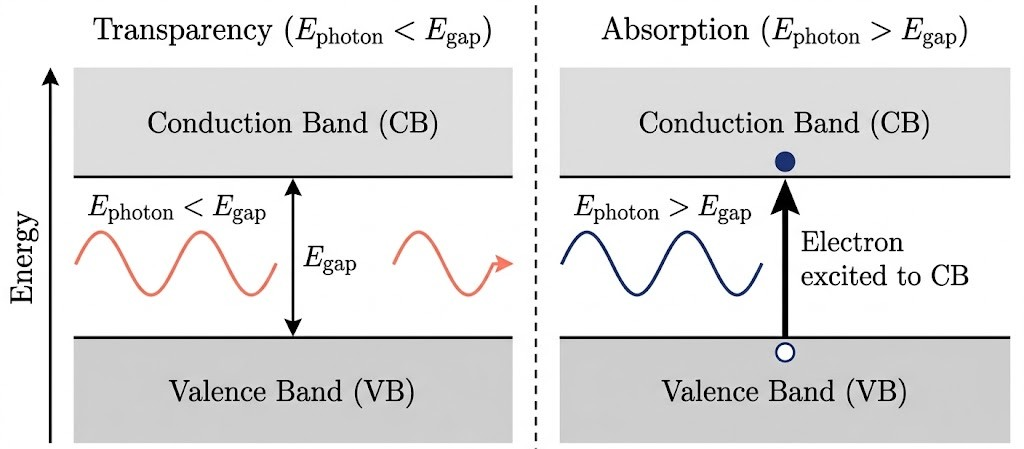
\includegraphics[width=0.6\textwidth]{Figures/Chapter 1/transparency_vs_absorption.jpg}
    \caption{Transparency vs. Absorption: Interaction depends on the photon energy relative to the band gap.}
\end{figure}

This chapter develops the first and most foundational of these frameworks — the classical electron oscillator. Before we begin, it helps to realize that no single model tells the whole story. To truly understand modern optoelectronics—and specifically the mechanisms that make a laser possible—we must move through three progressive levels of description:

\begin{enumerate}
    \item \textbf{Classical Electron Oscillator (Lorentz model):} We start here to build fundamental physical intuition. By treating the electron as a mass on a microscopic spring, we can derive macroscopic phenomena like the refractive index, chromatic dispersion, and optical absorption. However, because this model relies entirely on classical friction, it inherently forbids optical amplification (gain).
    \item \textbf{Einstein Transition Model:} To solve the gain problem, we replace the classical spring with discrete, quantized energy levels. By defining clear transition probabilities (the $A$ and $B$ coefficients), this model introduces stimulated emission and population inversion—the core engine driving every laser system.
    \item \textbf{Quantum-Mechanical Interpretation:} While the Einstein model assumes transitions happen, it doesn't explain \emph{why}. A full quantum mechanical approach (solving the Schrödinger equation) finally gives us the mathematical rigor needed to calculate atomic lifetimes and cross-sections directly from first principles.
\end{enumerate}

The physical picture of this interaction changes considerably depending on the material. In \textbf{gases} or lightly doped optical fibres, we analyze tightly bound electrons in isolated atoms, producing sharp, discrete spectral lines. In \textbf{semiconductors}, tight lattice packing blurs these energy levels into continuous \emph{energy bands}. Instead of isolated events, we track massive populations of free carriers jumping across a bandgap. Despite these architectural differences, the core physical principles developed here translate flawlessly to both environments.

\begin{motivation}[Journey Through Light-Matter Interaction]
    Understanding light-matter interaction requires establishing the physics step by step. We will start strictly with the \textbf{Classical Electron Oscillator} to build a rock-solid, intuitive picture of how a material bends and absorbs passing light waves. However, as we will prove at the end of this chapter, the classical model hits a mathematical dead end when trying to explain optical amplification. Recognizing this specific failure is what motivates our leap into the \textbf{Einstein Model} in the next chapter, ultimately paving the way to the full \textbf{Quantum Mechanical} treatment required to engineer real, operational devices.
\end{motivation}

\section{Model Comparison at a Glance}
Before we dive into the derivations, let's categorize exactly what each model does.

\begin{table}[H]
    \centering
    \begin{tabular}{@{} >{\raggedright\arraybackslash}p{0.22\textwidth} >{\raggedright\arraybackslash}p{0.34\textwidth} >{\raggedright\arraybackslash}p{0.36\textwidth} @{}}
        \toprule
        \textbf{Model}                & \textbf{Core Picture}                                     & \textbf{What It Explains / Misses}                                                   \\
        \midrule
        \textbf{Classical (Lorentz)}  & Bound electron behaves like a damped driven oscillator.   & Explains dispersion and absorption line shape; cannot explain true laser gain.       \\
        \textbf{Einstein (Two-level)} & Discrete levels $E_1, E_2$ and probabilistic transitions. & Explains spontaneous and stimulated emission, and population inversion.              \\
        \textbf{Quantum}              & Full state-level and field quantization.                  & Needed for precise transition rates, selection rules, and advanced photonics design. \\
        \bottomrule
    \end{tabular}
\end{table}

This table gives us our roadmap: we will start classically, discover a mechanism it fails to explain (gain), and step up into the Einstein model to resolve that gap. Now, let's derive the classical model from scratch.

\section{Classical Electron Oscillator (CEO): Lossless Start}
\subsection{Bound Electron as a Restoring-Force System}
Now we'll model our atom. Let's first build our physical intuition. Treat the atom as a heavy, fixed positive core (nucleus) and a much lighter bound electron orbiting it.

If the electron is slightly displaced from its equilibrium position by an external force (like an incoming electromagnetic wave), the Coulomb force pulls it back. By linearizing this Coulomb force around the equilibrium point, it behaves exactly like a mechanical spring system obeying Hooke's Law! This gives us our simple restoring force:
\begin{equation*}
    F_{\text{rest}} \approx -k_s x
\end{equation*}
where $k_s$ is the effective "spring constant" of the atom, $x$ is the displacement distance from equilibrium, and the negative sign indicates the force strictly opposes the displacement.

\begin{figure}[H]
    \centering
    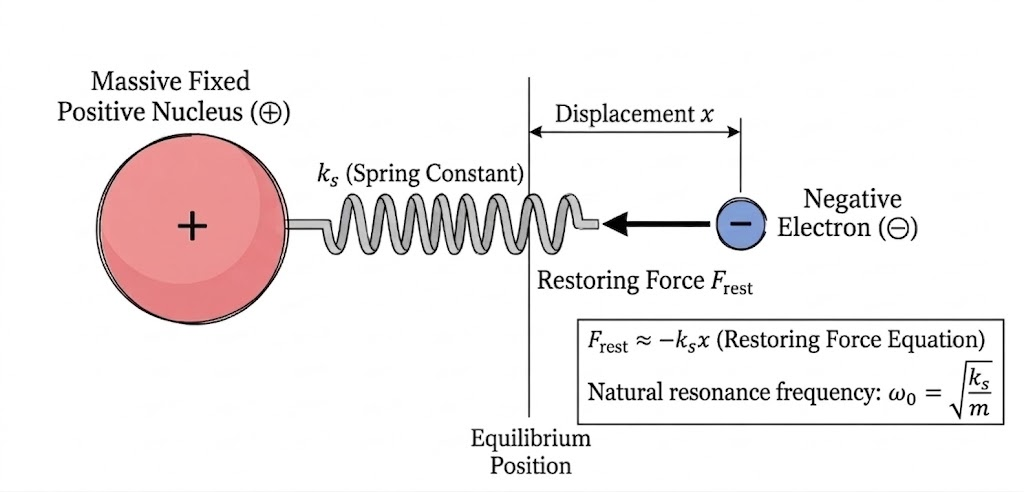
\includegraphics[width=0.6\textwidth]{Figures/Chapter 1/mechanical_atom_model.jpg}
    \caption{The Mechanical Atom Schematic: A bound electron modeled as a mass-spring system with a restoring force.}
\end{figure}

Now, applying Newton's second law ($F = m a$, where acceleration $a = \frac{d^2x}{dt^2}$) to this motion, we substitute our force to get our natural, unforced impulse response equation:
\begin{equation*}
    m\frac{d^2x}{dt^2} = -k_s x \quad \Rightarrow \quad m\frac{d^2x}{dt^2} + k_s x = 0
\end{equation*}
To isolate the highest derivative, we must divide the entire equation strictly by the mass $m$:
\begin{equation*}
    \frac{m}{m}\frac{d^2x}{dt^2} + \frac{k_s}{m} x = \frac{0}{m} \quad \Rightarrow \quad \frac{d^2x}{dt^2} + \left(\frac{k_s}{m}\right) x = 0
\end{equation*}
We now substitute a new constant $k_s/m$ with $\omega_0^2$. Substitute $\omega_0^2 = \frac{k_s}{m}$:
\begin{keyresult}
    \begin{equation}
        \frac{d^2x}{dt^2} + \omega_0^2 x = 0
    \end{equation}
\end{keyresult}
where $\omega_0 = \sqrt{\frac{k_s}{m}}$ is explicitly defined as the \textbf{natural frequency} (or resonance frequency) of the bound electron.

\textbf{Interpretation:} If perturbed, the electron will simply oscillate back and forth forever at this specific frequency $\omega_0$. Because this is a standard harmonic oscillator equation of the form $x'' + \omega_0^2 x = 0$, the mathematical solution is purely sinusoidal. Let's write the solution explicitly:
\begin{equation*}
    x(t)=A\cos(\omega_0 t+\phi)
\end{equation*}
where $A$ is the amplitude of the displacement, and $\phi$ is the phase.

Ultimately, the basic structure of an atom naturally acts like a spring mass system, producing a pure, endless oscillation when disturbed at its resonance frequency $\omega_0$.

\begin{keyinsight}[On Thermal Energy]
    One might ask: doesn't thermal energy already displace the electron and cause oscillations? Recall that at temperature $T$, each degree of freedom carries an average thermal energy of $\frac{1}{2}k_B T$. This thermal energy gives the electron a random thermal velocity, but it does \textbf{not} produce coherent oscillations. The random thermal motion averages to zero displacement over time. Only an externally applied coherent field (such as an electromagnetic wave) can drive a sustained, phase-locked oscillation of the electron cloud.
\end{keyinsight}

\subsection{Why This Is Incomplete}
While simple, this lossless model is critically flawed and not physically realistic. It predicts an infinitely sharp resonance (meaning the atom interacts with light \emph{only} at exactly $\omega_0$) and assumes the electron will oscillate forever without losing any energy. In reality, real atoms lose energy through radiation (the antenna effect) and through collisions (lattice vibrations). We must now upgrade our model to incorporate these losses.

\section{Damping, Lifetime, and Broadening}
\subsection{The Damped Oscillator Equation}
To account for these energy losses, we must introduce an equivalent frictional force into our equation. Recall from basic electromagnetics that any electron undergoing acceleration will radiate electromagnetic waves, losing energy. Additionally, electrons scatter off other atoms in the lattice.

So, we model this by adding a damping force that is strictly proportional to the electron's velocity. Let $b$ be the friction factor:
\begin{equation*}
    m\frac{d^2x}{dt^2} + \underbrace{b\frac{dx}{dt}}_{\text{damping}} + k_s x = 0
\end{equation*}

Once again, to solve this, we must isolate the highest order derivative by dividing the entire equation by the electron mass $m$:
\begin{equation*}
    \frac{m}{m}\frac{d^2x}{dt^2}+\frac{b}{m}\frac{dx}{dt}+\frac{k_s}{m}x= \frac{0}{m} \quad \Rightarrow \quad \frac{d^2x}{dt^2}+\left(\frac{b}{m}\right)\frac{dx}{dt}+\left(\frac{k_s}{m}\right)x=0
\end{equation*}
We now define two fundamental substitutions. Substitute $\eta = \frac{b}{m}$ (defined as the damping coefficient) and substitute $\omega_0^2 = \frac{k_s}{m}$ (our natural frequency squared). This yields our new governing equation:
\begin{equation*}
    \frac{d^2x}{dt^2}+\eta\frac{dx}{dt}+\omega_0^2x=0
\end{equation*}

To solve this linear homogeneous differential equation with constant coefficients, we assume a solution of the form $x(t) = Ae^{st}$, leading directly to the characteristic equation:
\begin{equation*}
    s^2 + \eta s + \omega_0^2 = 0
\end{equation*}
We apply the quadratic formula $s = \frac{-B \pm \sqrt{B^2 - 4AC}}{2A}$. Substitute $A=1$, $B=\eta$, and $C=\omega_0^2$:
\begin{equation*}
    s = \frac{-\eta \pm \sqrt{\eta^2 - 4(1)(\omega_0^2)}}{2(1)} \quad \Rightarrow \quad s = -\frac{\eta}{2} \pm \frac{\sqrt{\eta^2 - 4\omega_0^2}}{2} = -\frac{\eta}{2} \pm \sqrt{\left(\frac{\eta}{2}\right)^2 - \omega_0^2}
\end{equation*}

The behavior of the system depends entirely on the value inside this square root. We must define the cases:
\begin{enumerate}
    \item \textbf{Case 1: Overdamped ($\eta/2 > \omega_0$).} The term $\left(\frac{\eta}{2}\right)^2 - \omega_0^2$ is strictly positive. The square root evaluates to a real number. The roots $s$ are purely real and negative. The electron just slowly decays exponentially back to equilibrium without ever crossing the center.
    \item \textbf{Case 2: Critically Damped ($\eta/2 = \omega_0$).} The term inside the square root is exactly zero. The roots are equal ($s=-\eta/2$). The electron returns to equilibrium as fast as possible without oscillating.
    \item \textbf{Case 3: Underdamped ($\eta/2 < \omega_0$).} The term $\left(\frac{\eta}{2}\right)^2 - \omega_0^2$ is negative. The damping is relatively weak compared to the restoring force. When we take the square root of a negative number, it forces $s$ to be complex. A complex exponent transforms mathematically into a real exponentially decaying sinusoid.
\end{enumerate}

\begin{figure}[H]
    \centering
    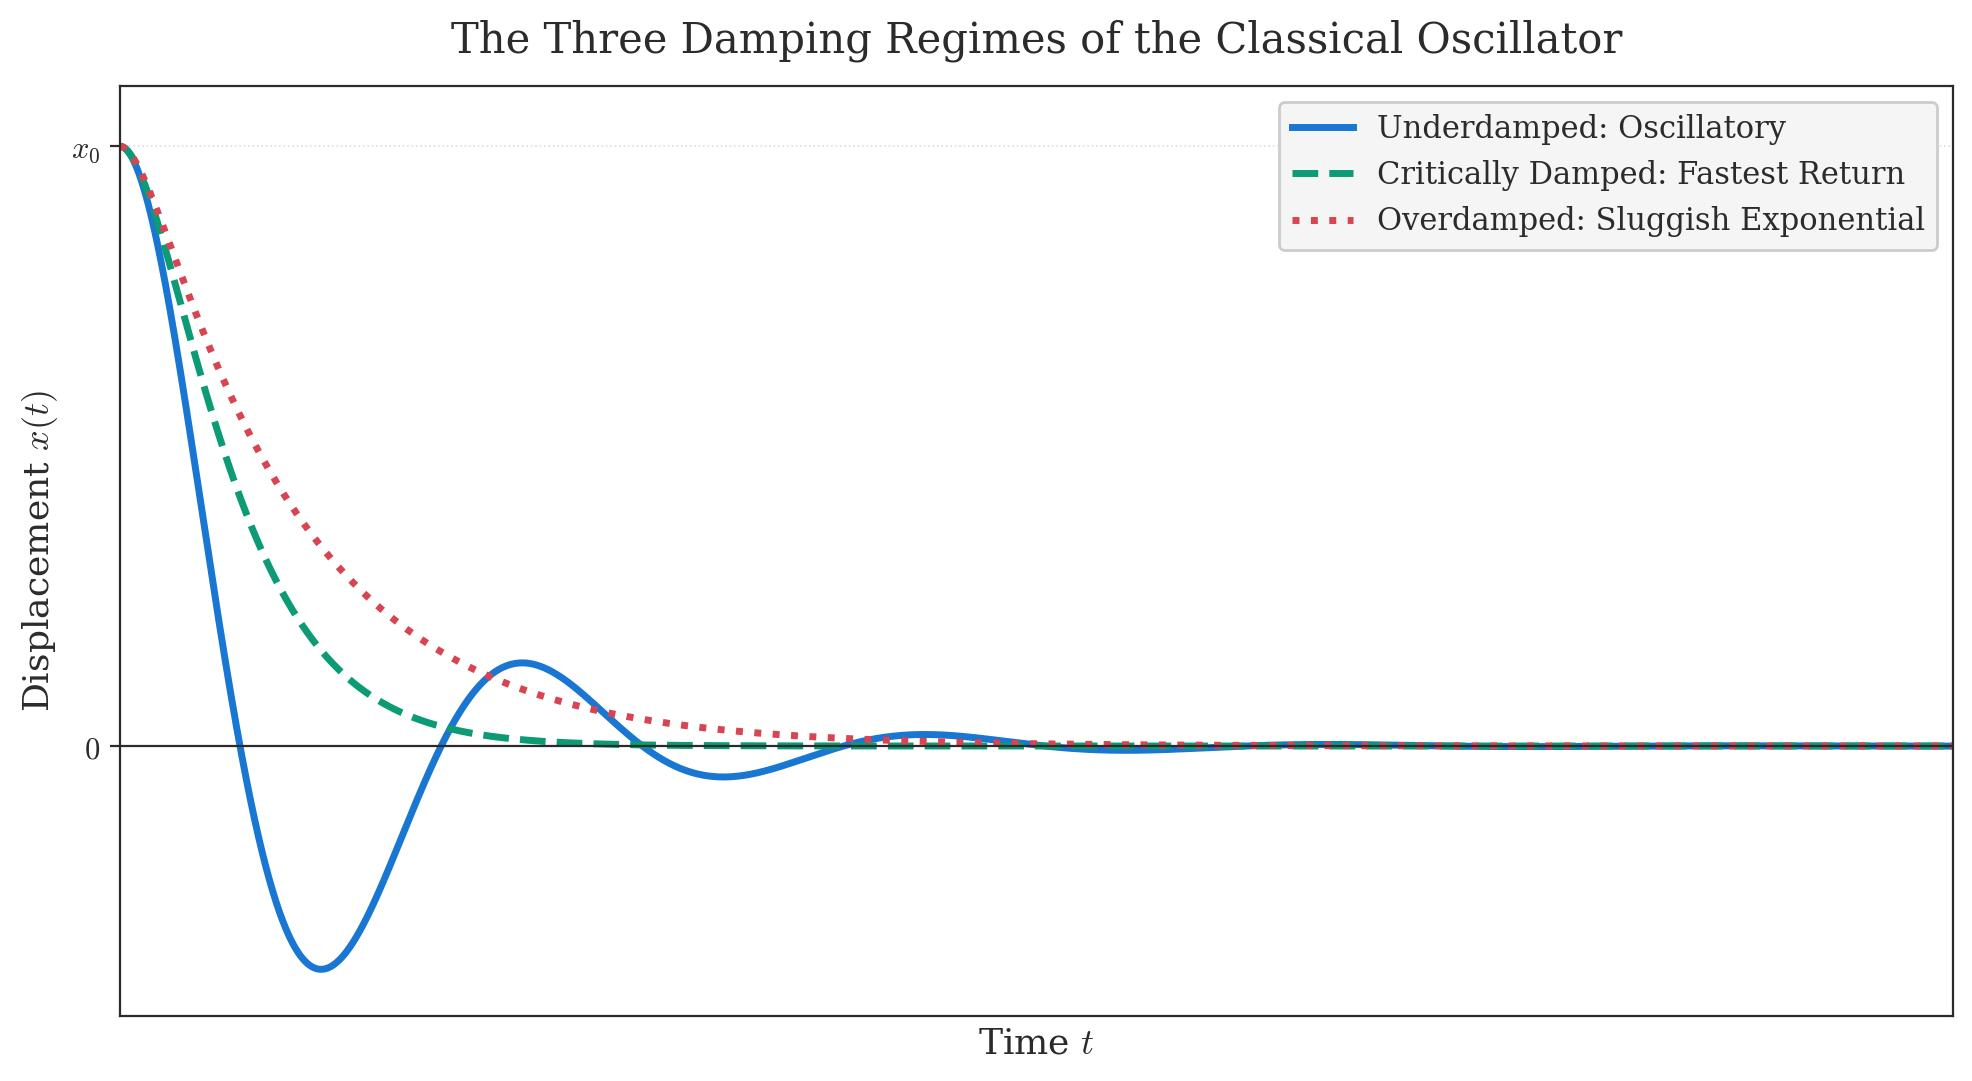
\includegraphics[width=0.65\textwidth]{Figures/Chapter 1/three_damping_regimes.jpg}
    \caption{The Three Damping Regimes: Comparison of the displacement decay for overdamped, critically damped, and underdamped oscillators.}
\end{figure}

Since we are dealing with optical phenomena where damping is relatively small, we always assume the \textbf{Underdamped} case. Thus, our solution becomes an exponentially decaying oscillation:
\begin{equation*}
    x(t)=A e^{-\eta t/2}\cos(\omega_d t+\phi),
\end{equation*}
where $\omega_d$ is the damped natural frequency, defined as:
\begin{equation*}
    \omega_d=\sqrt{\omega_0^2-\left(\frac{\eta}{2}\right)^2}
\end{equation*}

\begin{figure}[H]
    \centering
    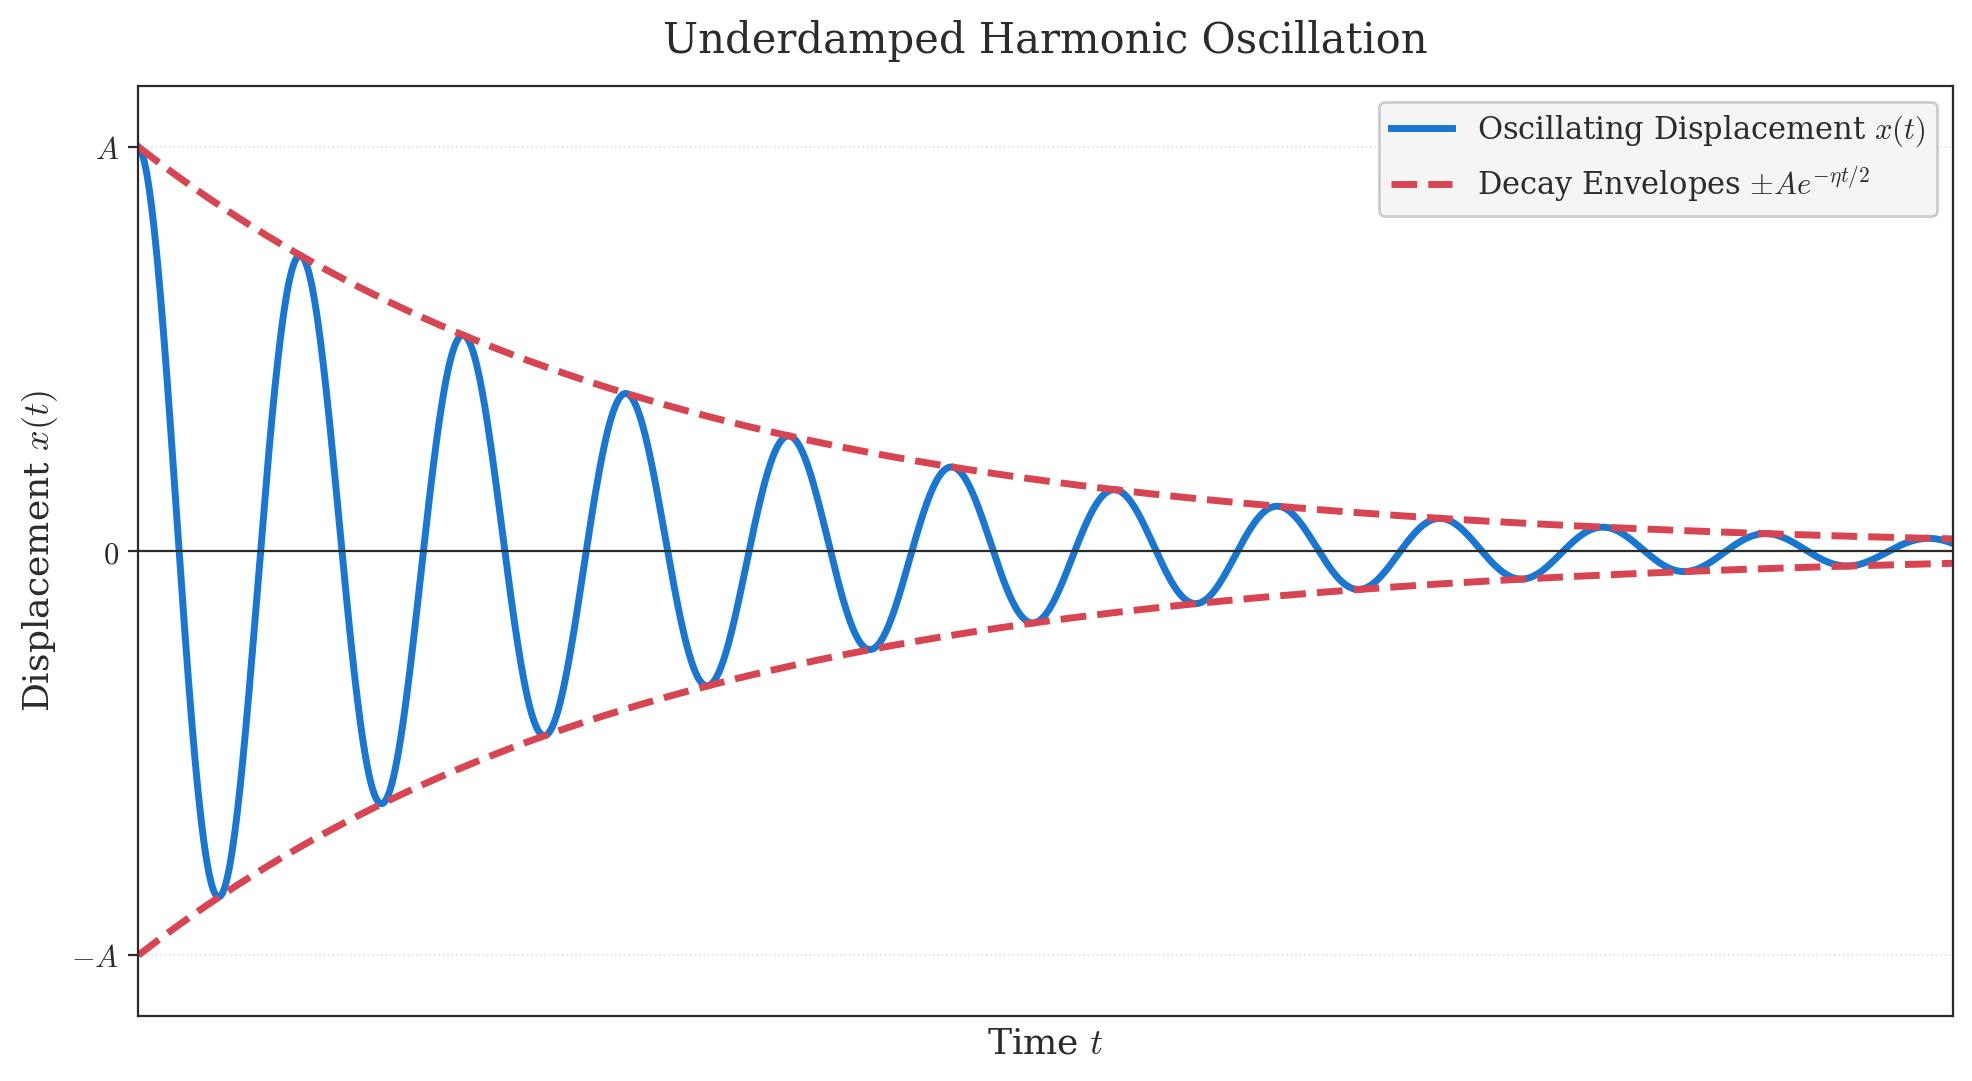
\includegraphics[width=0.65\textwidth]{Figures/Chapter 1/underdamped_oscillation.jpg}
    \caption{Underdamped Oscillation: The electron's displacement oscillates inside an exponentially decaying envelope.}
\end{figure}

\begin{keyinsight}[Justifying the Underdamped Assumption]
    Is the underdamped assumption ($\eta/2 < \omega_0$) valid for optical materials? Yes. The displacement solution $x(t) = A e^{-\eta t/2}\cos(\omega_d t+\phi)$ explicitly shows that the coefficient $\eta$ acts purely as a decay rate for the amplitude envelope, while $\omega_0$ (via the damped frequency $\omega_d=\sqrt{\omega_0^2-(\eta/2)^2}$) sets the rapid oscillation. For visible light, the natural oscillation frequency of an electron is immense: $\omega_0 \approx 10^{15}$ rad/s. In contrast, the atomic ``friction'' causing the oscillation to decay acts much more slowly. The amplitude typically takes a few nanoseconds to visibly shrink, making the decay rate roughly $\eta \approx 10^9$ s$^{-1}$. Because $10^9 \ll 10^{15}$ (meaning $\eta \ll \omega_0$), the electron will ring for millions of cycles before the envelope dies out. Therefore, atomic electron oscillators are strictly underdamped!
\end{keyinsight}

\subsection{Energy Decay and the Concept of "Lifetime"}
Now let's talk about the energy of this system. The total energy $U$ of our Classical Electron Oscillator (CEO) is the sum of its potential and kinetic energy.

First, let's derive the potential energy stored in our ideal spring model. The restoring force of the spring is $F_s = -k_s x$. The potential energy (P.E) is the work done against this force to stretch the spring from equilibrium ($x=0$) to a displacement $x$:
\begin{equation*}
    \text{P.E} = -\int_0^x F_s \, dx' = \int_0^x k_s x' \, dx' = \frac{1}{2} k_s x^2
\end{equation*}
The total energy $U$ maxes out completely as potential energy exactly when the kinetic energy is zero (meaning its velocity is zero at the peak of its swing, where $x = \text{Amplitude } A$):
\begin{equation*}
    U = \text{P.E} + \text{K.E} \approx \max (\text{P.E}) \Big|_{K.E = 0} = \frac{1}{2} k_s A^2
\end{equation*}
Recall from our displacement solution that the amplitude decays as $x_{\text{peak}} \propto e^{-\eta t/2}$. If we plug this amplitude constraint into our energy equation:
\begin{equation*}
    U(t) \propto \left(e^{-\eta t/2}\right)^2 = e^{-\eta t}
\end{equation*}
Thus, the total energy $U$ decays exponentially at a rate of $\eta$:
\begin{equation*}
    U(t)=U(0)e^{-\eta t}
\end{equation*}

We now define a critical metric called the \textbf{Total Lifetime ($\tau_t$)}—sometimes denoted as $\eta^{-1}$. This term represents the specific amount of time it takes for the system's energy to decay to exactly $1/e$ ($\approx 37\%$) of its initial starting value $U(0)$:
\begin{equation*}
    \text{If } U(\tau_t) = U(0)e^{-1}, \text{ then explicitly } \tau_t = \frac{1}{\eta}.
\end{equation*}

\begin{figure}[H]
    \centering
    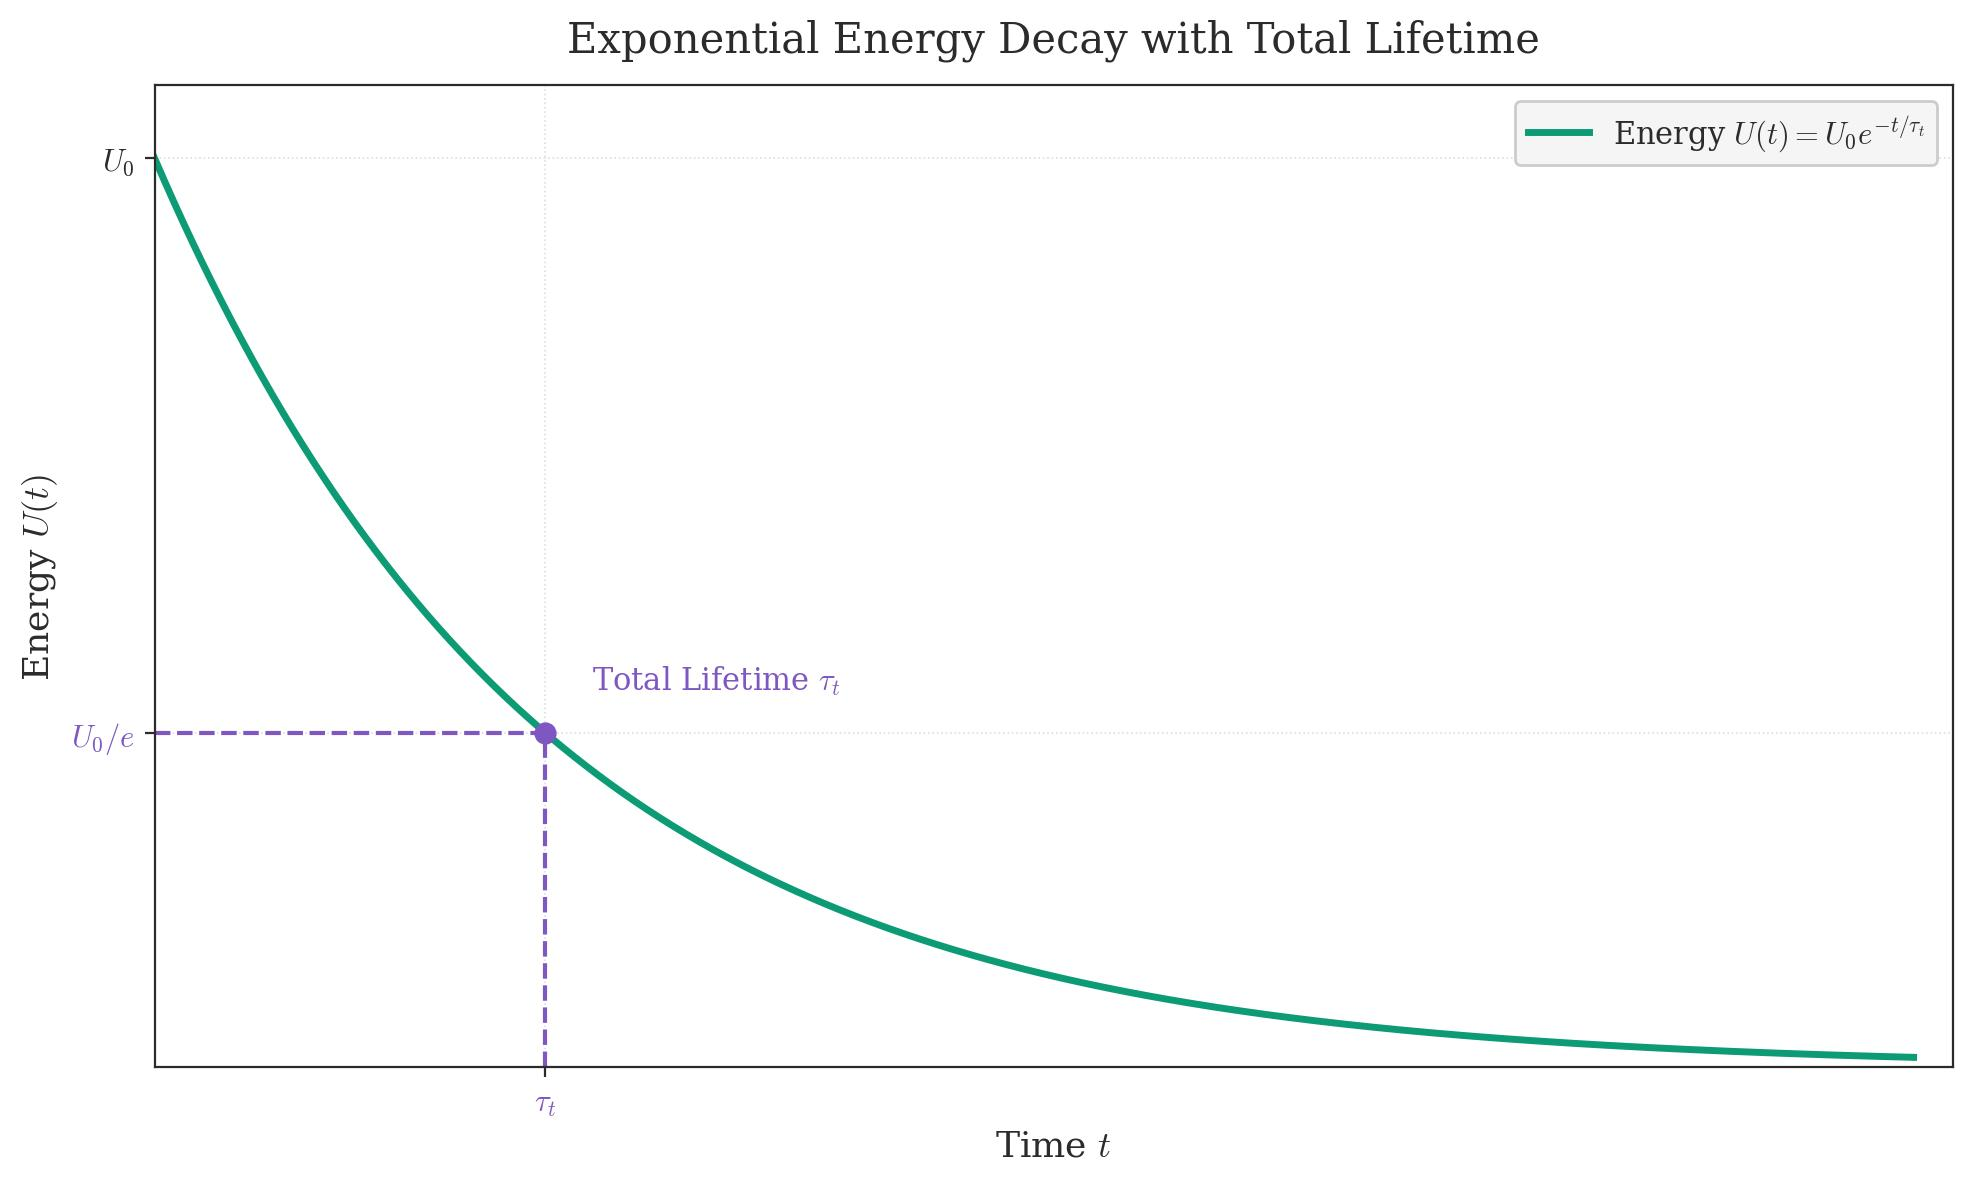
\includegraphics[width=0.65\textwidth]{Figures/Chapter 1/energy_decay_profile.jpg}
    \caption{Energy Decay Profile: Total energy decays exponentially, with the lifetime $\tau_t$ marking the $1/e$ point.}
\end{figure}

In general, the atom has multiple ways to "relax" and lose this energy. We distinguish two primary relaxation channels. Because these events occur independently, their rates add together. The fastest relaxation method always dominates the total lifetime:
\begin{equation*}
    \frac{1}{\tau_t}=\frac{1}{\tau_r}+\frac{1}{\tau_{nr}}
\end{equation*}
We fully explore both channels below:
\begin{itemize}
    \item \textbf{Radiative Lifetime ($\tau_r$):} The average time an excited atom takes to release its stored energy by emitting a photon. It fundamentally measures how strongly the atom couples to the electromagnetic field — a short $\tau_r$ means the atom radiates quickly and efficiently, while a long $\tau_r$ means the atom is weakly coupled and holds its energy for a long time before any emission occurs. This is governed by the relation:
          \begin{equation*}
              \tau_r = \frac{6 \pi \epsilon m c^3}{e^2 \omega_0^2}, \quad \text{where } \epsilon = n^2 \varepsilon_0, \ c = \frac{c_0}{n}
          \end{equation*}
    \item \textbf{Non-Radiative Lifetime ($\tau_{nr}$):} The atom relaxes through "collisions" without ever emitting light. Examples include hitting the surrounding atomic lattice (creating lattice vibrations/phonons) or Auger recombination where the energy is kicked directly to another nearby electron.
\end{itemize}

\begin{figure}[H]
    \centering
    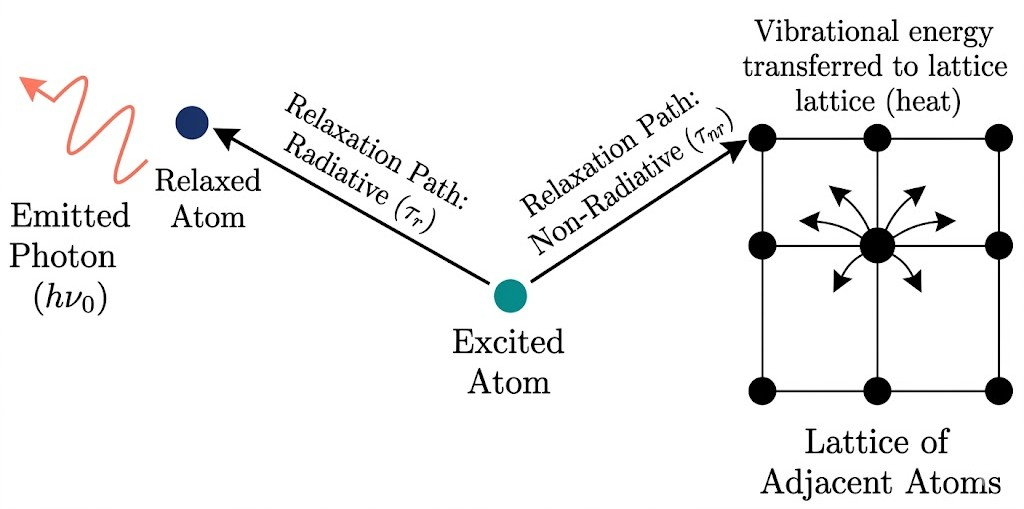
\includegraphics[width=0.6\textwidth]{Figures/Chapter 1/relaxation_paths.jpg}
    \caption{Relaxation Paths: An excited atom can decay purely via radiative mechanisms (photon emission) or non-radiative multi-phonon mechanisms (lattice heating).}
\end{figure}

The physical takeaway here is that the friction parameter $\eta$ governs the total lifetime $\tau_t$ of the atom's excited state, combining both radiative light-emitting effects and non-radiative collisional effects.

\subsection{Broadening Insight: Why Damping Creates Bandwidth}
To master light-matter interaction, we must understand how damping changes the frequency response. Without damping, the interaction between light and matter happens strictly at an infinitely sharp impulse at $\omega_0$.

However, because of the damping mechanisms (both radiative and collisional) causing energy loss, the spectral response broadens. This phenomenon is called \textbf{Broadening}.

\textbf{What exactly is Broadening?:} Stronger damping ($\eta \uparrow$) means the atom loses energy faster, meaning a heavily decreased lifetime $\tau_t$. In the frequency domain, this shorter lifetime translates into a \emph{wider} resonance peak.
If the peak is wider, it means the atom can interact with a wider "Bandwidth" of frequencies surrounding $\omega_0$, though its peak response will inevitably be lower.

Now that we fully understand the internal mechanics of the single atom, we must apply an external field to see how it forces the atom to behave.

\section{Forced Response to an Optical Field}
\subsection{Lorentz Force Simplification}
Now we'll see what happens when we expose our damped electron to light. Recall that light is an electromagnetic wave, meaning it carries both an electric field $\bm{E}$ and a magnetic field $\bm{B}$.

If we shine this wave onto our electron, it exerts a force known as the Lorentz force. The total Lorentz force $\bm{F}$ exerted by an electromagnetic wave on a charge $q$ moving with velocity $\bm{v}$ is:
\begin{equation*}
    \bm{F}=\bm{F}_e+\bm{F}_m=q\bm{E}+q(\bm{v}\times\bm{B}),
\end{equation*}
where $q$ is the charge ($-e$ for an electron), $\bm{E}$ is the electric field vector, $\bm{v}$ is the electron velocity vector, and $\bm{B}$ is the magnetic field vector.

\begin{keyinsight}[Why the Magnetic Force is Negligible]
    For a plane wave in a medium, the ratio of the magnetic field magnitude to the electric field magnitude is strictly determined by the phase velocity $v_p$ of the light:
    \begin{equation*}
        \frac{|\bm{B}|}{|\bm{E}|} = \frac{1}{v_p} \quad \Rightarrow \quad |\bm{B}| = \frac{|\bm{E}|}{v_p},
    \end{equation*}
    where the phase velocity $v_p$ is defined by the free-space speed of light $c_0 \approx 3 \times 10^8$ m/s as $v_p = \frac{c_0}{n}$, with $n$ being the refractive index of the medium.

    Now let's compare the magnitude of the magnetic force part $|\bm{F}_m| = |q(\bm{v}\times\bm{B})| \approx q v |\bm{B}|$ (assuming perpendicular velocity to maximize the possible cross product force) to the basic electric force part $|\bm{F}_e| = q |\bm{E}|$. We structure their ratio explicitly:
    \begin{equation*}
        \frac{|\bm{F}_m|}{|\bm{F}_e|} = \frac{q v |\bm{B}|}{q |\bm{E}|} = \frac{v |\bm{B}|}{|\bm{E}|}
    \end{equation*}
    Substitute $|\bm{B}| = \frac{|\bm{E}|}{v_p}$ into the numerator:
    \begin{equation*}
        \frac{|\bm{F}_m|}{|\bm{F}_e|} = \frac{v \left(\frac{|\bm{E}|}{v_p}\right)}{|\bm{E}|} = \frac{v}{v_p}
    \end{equation*}
    Substitute $v_p = \frac{c_0}{n}$:
    \begin{equation*}
        \frac{|\bm{F}_m|}{|\bm{F}_e|} = \frac{v}{(c_0/n)} = \frac{n v}{c_0}
    \end{equation*}
    For standard optical index materials ($n \approx 1$ to $4$), since bound electron velocities are highly non-relativistic (which rigorously defines the condition $v \ll c_0$), the fraction $v/c_0$ evaluates extremely close to zero. Therefore, if $v \ll c_0$, then the ratio $|\bm{F}_m|/|\bm{F}_e| \to 0$, meaning the magnetic force is completely negligible compared to the electric force.
\end{keyinsight}

Because we established the strict condition $v \ll c_0$, we can safely drop the entire $\bm{F}_m$ vector from the total Lorentz force and assume a purely \textbf{one-dimensional} external electric driving force:
\begin{equation*}
    \bm{F}\approx \bm{F}_e = q\bm{E} = -e\bm{E}
\end{equation*}

For all standard linear optics where electrons aren't moving anywhere near the speed of light, we only need to worry about the electric push of the light wave, ignoring its magnetic tug entirely.

\subsection{The Driven Equation: Adding an External Wave}
So far, we looked at how the electron naturally behaves under damping without external influence. Now, let's force the system. We will substitute our external force $F \approx -e E(t)$ into the right-hand side of our damped differential equation (replacing the zero):
\begin{equation*}
    m\frac{d^2x}{dt^2}+b\frac{dx}{dt}+k_s x = -e E(t)
\end{equation*}
Dividing entirely by $m$ and using our substitutions $\eta = b/m$ and $\omega_0^2 = k_s/m$, we construct the fundamental equation of linear optics:
\begin{keyresult}
    \begin{equation}
        \frac{d^2x}{dt^2}+\eta\frac{dx}{dt}+\omega_0^2x=-\frac{e}{m}E(t)
    \end{equation}
\end{keyresult}

Because our optical field strongly oscillates, we must solve this in the \textbf{Phasor Domain}.

If we assume the incoming light wave oscillates at a steady driving frequency $\omega$ in the form $E(t)=\Re\{E_0 e^{j\omega t}\}$, then because the system is perfectly linear, the steady-state displacement $x(t)$ must also oscillate at that exact same frequency $\omega$, taking the form $x(t)=\Re\{x_0 e^{j\omega t}\}$.

Substitute $x(t) = x_0 e^{j\omega t}$ into our differential equation. This allows us to convert time derivatives algebraically: $\frac{d}{dt} \to j\omega$ and $\frac{d^2}{dt^2} \to (j\omega)^2 = -\omega^2$.
\begin{equation*}
    -\omega^2 x_0 e^{j\omega t} + \eta (j\omega) x_0 e^{j\omega t} + \omega_0^2 x_0 e^{j\omega t} = -\frac{e}{m} E_0 e^{j\omega t}
\end{equation*}
The exponential terms $e^{j\omega t}$ explicitly cancel from every single term on both sides. Next, we group the terms on the left side to factor out $x_0$:
\begin{equation*}
    x_0(-\omega^2) + x_0(j\eta\omega) + x_0(\omega_0^2) = -\frac{e}{m} E_0 \quad \Rightarrow \quad x_0 \left(-\omega^2+j\eta\omega + \omega_0^2 \right) = -\frac{e}{m} E_0
\end{equation*}
This perfectly simplifies to our final solution for the phasor displacement $x_0$:
\begin{keyresult}
    \begin{equation}
        x_0=-\frac{e}{m}\frac{E_0}{\omega_0^2-\omega^2+j\eta\omega}
    \end{equation}
\end{keyresult}

\begin{keyinsight}[The Two Frequencies: $\omega_0$ vs. $\omega$]
    It is crucial to never confuse the two distinct frequencies now present in the equation for $x_0$:
    \begin{itemize}
        \item \textbf{Natural Frequency ($\omega_0$):} This is the \emph{internal} property of the atom itself, determined by the ``spring stiffness'' $k_s$ binding the electron. It is the frequency the electron inherently ``wants'' to vibrate at.
        \item \textbf{Driving Frequency ($\omega$):} This is the \emph{external} property of the incoming electromagnetic light wave. It is the frequency at which the light physically \emph{forces} the electron to move.
    \end{itemize}
    The difference between them, called the \textbf{Detuning} ($\Delta\omega = \omega - \omega_0$), dictates the entire interaction. When the external push matches the natural rhythm ($\omega \approx \omega_0$), we hit resonance, causing massive energy transfer.
\end{keyinsight}

What does this equation tell us? It proves that the electron's movement $x_0$ depends enormously on the denominator.
We must explicitly consider the resonance cases:
\begin{enumerate}
    \item \textbf{Case 1: Low-frequency drive ($\omega \ll \omega_0$).} The $\omega_0^2$ term dominates. The displacement $x_0$ is completely real and simply tracks the applied field in-phase. The atom acts purely like a perfect rigid spring.
    \item \textbf{Case 2: High-frequency drive ($\omega \gg \omega_0$).} The $-\omega^2$ term dominates. The displacement is real but negative (out of phase by 180 degrees). The electron cannot move fast enough to keep up with the light, limited purely by its mass inertia.
    \item \textbf{Case 3: On Resonance ($\omega = \omega_0$).} The $\omega_0^2$ and $-\omega^2$ terms cancel each other perfectly! The denominator becomes purely imaginary ($j\eta\omega$). The displacement $x_0$ is purely imaginary (out of phase by exactly 90 degrees), and its amplitude is limited entirely by the friction $\eta$. This is where maximum energy is absorbed.
\end{enumerate}

\begin{figure}[H]
    \centering
    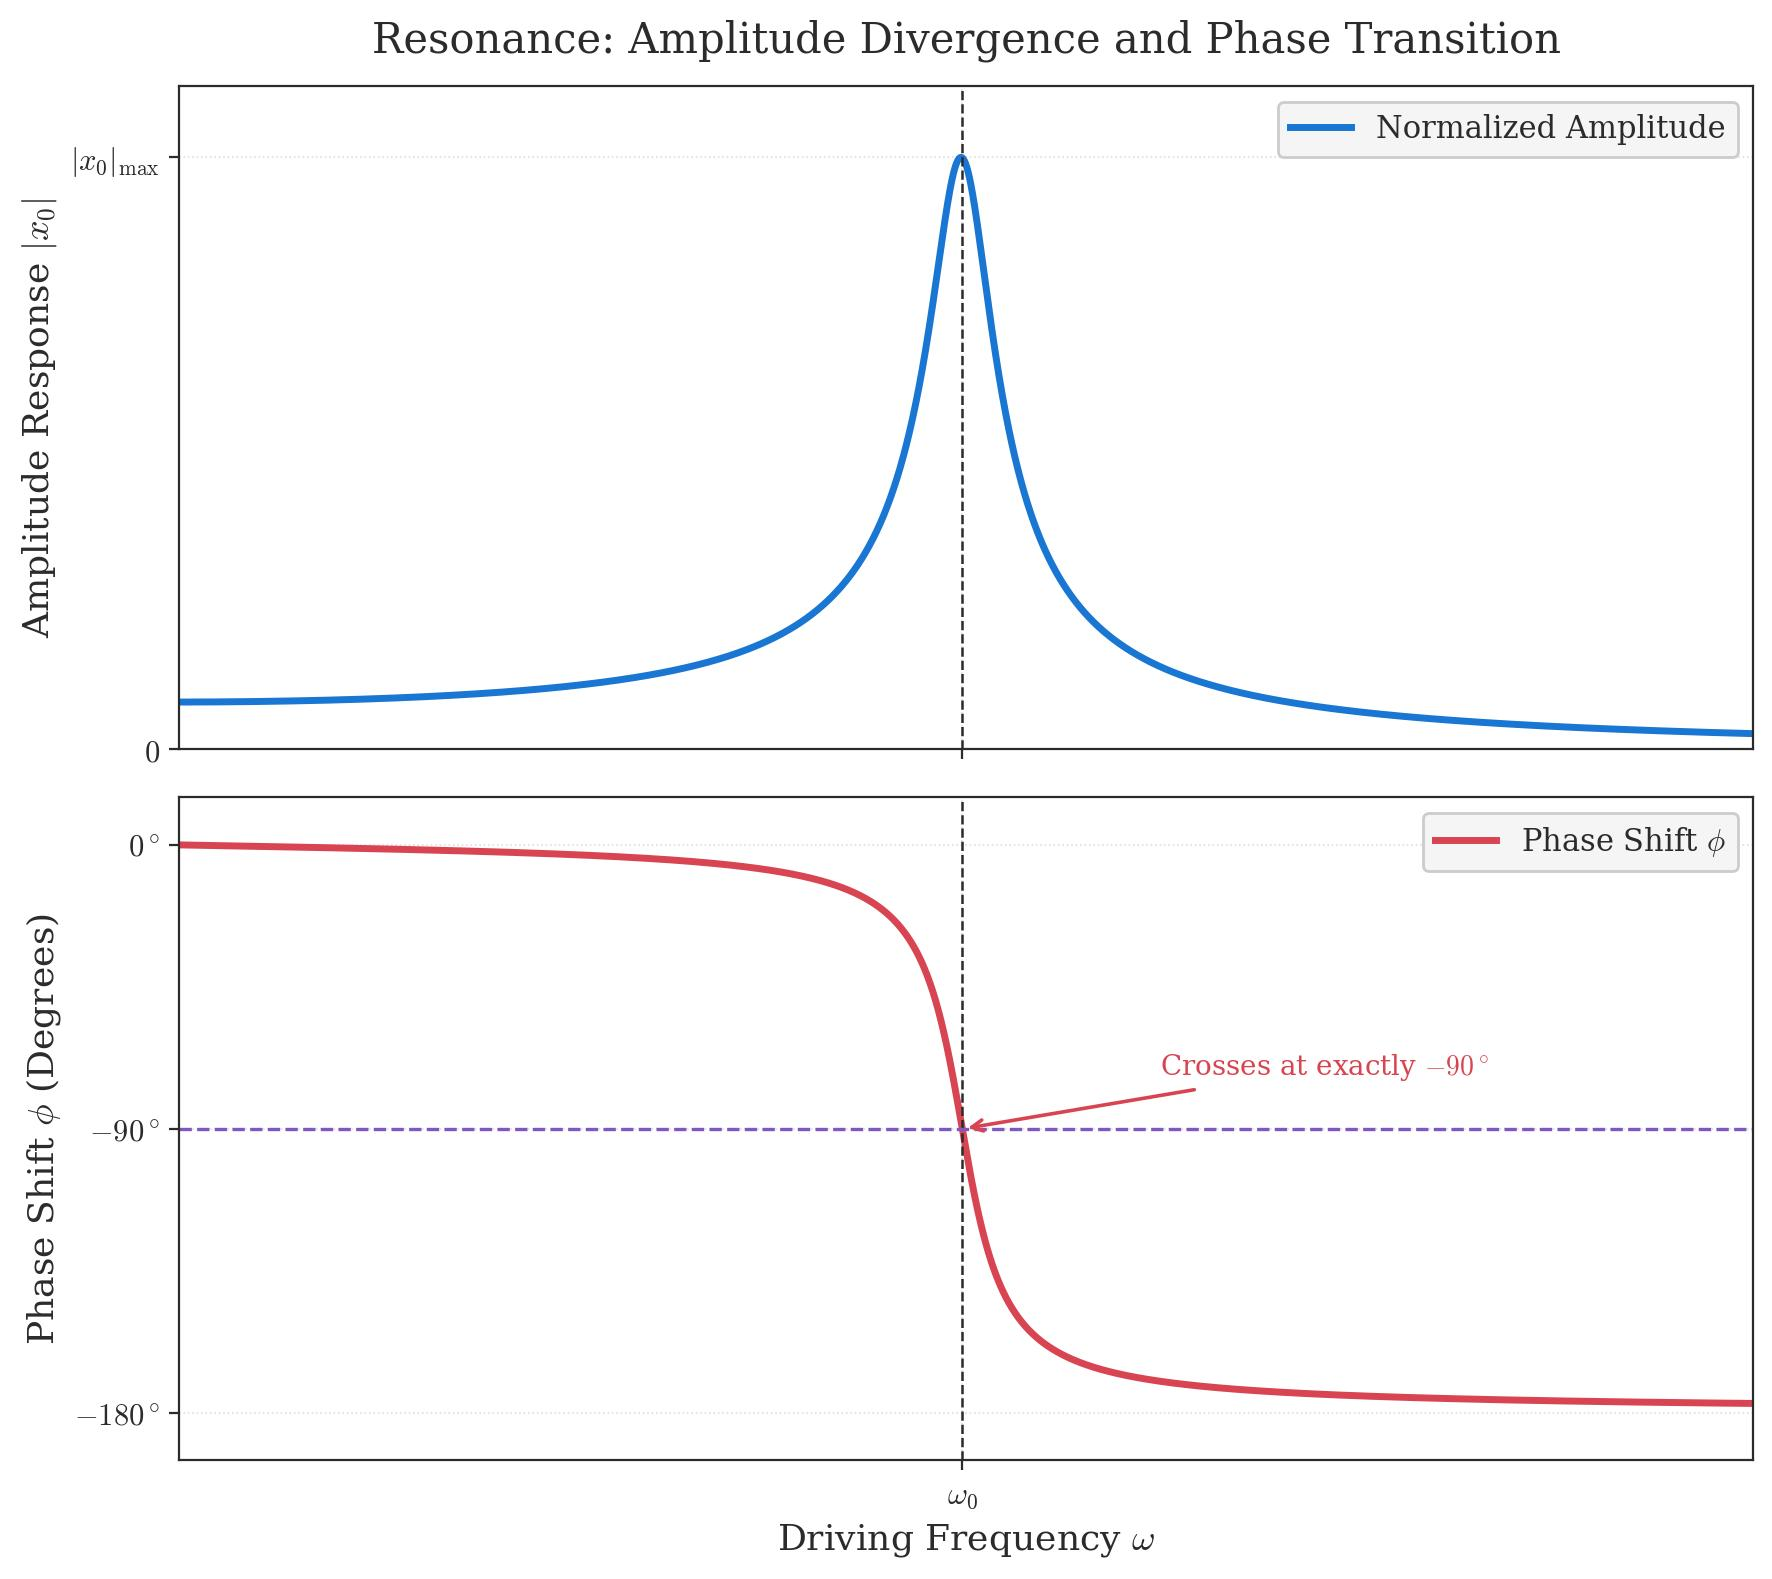
\includegraphics[width=0.65\textwidth]{Figures/Chapter 1/resonance_amplitude_phase.jpg}
    \caption{Resonance Effects: Amplitude and phase shift of the electron's displacement as a function of the external driving frequency.}
\end{figure}

\begin{keyinsight}[Physical Meaning of Phase and Energy Absorption]
    To pump maximum energy into a swing, you must push exactly when it moves forward—your force must be perfectly in-sync with its \emph{velocity}, not its position. Push out of sync, and you cancel your own work. This exact principle governs light-matter energy transfer: the average power absorbed by the atom strictly requires the electron's velocity to be in-phase with the light's driving force ($\langle P \rangle \propto \langle F \cdot v \rangle$).

    In the purely phasor domain, velocity is simply the time-derivative of position ($v_0 = j\omega x_0$). Substituting our displacement equation, we find the explicit velocity phasor:
    \begin{equation*}
        v_0 = j\omega \left( -\frac{e}{m}\frac{E_0}{\underbrace{\omega_0^2 - \omega^2 + j\eta\omega}_{\text{determines the phase}}} \right)
    \end{equation*}
    The $j$ multiplier mathematically dictates that velocity is always strictly $+90^\circ$ ahead of displacement. Therefore, to align this velocity perfectly with a purely real driving force, the denominator itself must provide exactly $-90^\circ$ of phase lag (meaning the denominator must be purely imaginary) to cancel out the $j$ in the numerator. Let's evaluate this across our regimes:

    \begin{itemize}
        \item \textbf{Off-Resonance ($\omega \ll \omega_0$ or $\omega \gg \omega_0$):} The real terms ($\omega_0^2$ or $-\omega^2$) completely dominate the denominator, making it purely real. Because the denominator is real, the $j$ in the numerator survives, forcing the final velocity $v_0$ to be purely imaginary.
              \begin{equation*}
                  \text{Force and Velocity are } 90^\circ \text{ out of phase} \quad \Rightarrow \quad \langle P \rangle = 0
              \end{equation*}
              The atom jiggles elastically, absorbing energy and instantly returning it to the field. Light passes through completely unabsorbed.

        \item \textbf{On Resonance ($\omega = \omega_0$):} The real terms exactly cancel ($\omega_0^2 - \omega^2 = 0$). The denominator collapses to the purely imaginary $j\eta\omega$. When we plug this into our velocity equation, the complex $j$ in the numerator and the $j$ in the denominator perfectly annihilate each other!
              \begin{equation*}
                  v_0 = j\omega \left( -\frac{e}{m}\frac{E_0}{j\eta\omega} \right) = -\frac{e}{m}\frac{E_0}{\eta} \quad \Rightarrow \quad v_0 \text{ is purely \emph{real}}
              \end{equation*}
              Velocity is now perfectly in-phase with the driving force! The light constantly does positive work, irreversibly dumping its energy into the atom: $\langle P \rangle > 0$. This is the perfect resonance absorption condition—the atom acts as an uninterrupted energy sink.
    \end{itemize}
\end{keyinsight}

Before we can pull these microscopic insights into the macroscopic world, we must do one mathematical housekeeping step: explicitly separating the electron's displacement phasor ($x_0$) into purely real ($x'$) and entirely imaginary ($x''$) components. This split is the strict mathematical root of why a material can simultaneously shift the phase of light while absorbing its energy.

We start directly from the base equation for the displacement amplitude we just derived in the classical model:
\begin{equation*}
    x_0 = -\frac{e}{m} \left[ \frac{E_0}{(\omega_0^2 - \omega^2) + j\eta\omega} \right]
\end{equation*}

To isolate the real and imaginary parts, we must clear the complex unit $j$ from the denominator. We do this by multiplying the numerator and denominator by the complex conjugate of the denominator, $(\omega_0^2 - \omega^2) - j\eta\omega$:
\begin{equation*}
    x_0 = -\frac{e}{m} \left[ \frac{E_0}{(\omega_0^2 - \omega^2) + j\eta\omega} \cdot \frac{(\omega_0^2 - \omega^2) - j\eta\omega}{(\omega_0^2 - \omega^2) - j\eta\omega} \right] \quad \Rightarrow \quad x_0 = -\frac{e}{m} \left[ \frac{E_0[(\omega_0^2 - \omega^2) - j\eta\omega]}{(\omega_0^2 - \omega^2)^2 + (\eta\omega)^2} \right]
\end{equation*}

We can now cleanly separate the fraction into a purely real part ($x'$) and a purely imaginary part ($x''$), defined such that $x_0 = x' + jx''$.

The real part $x'$ gives the in-phase displacement (which will ultimately scale up to drive the macroscopic refractive index), and the imaginary part $x''$ gives the out-of-phase displacement (which will dictate optical absorption):
\begin{keyresult}
    \begin{gather}
        x' = -\frac{e}{m} \left[ \frac{E_0(\omega_0^2 - \omega^2)}{(\omega_0^2 - \omega^2)^2 + (\eta\omega)^2} \right] \quad \text{(Real Part $\to$ In-Phase Displacement)} \\[1ex]
        x'' = \frac{e}{m} \left[ \frac{E_0(\eta\omega)}{(\omega_0^2 - \omega^2)^2 + (\eta\omega)^2} \right] \quad \text{(Imaginary Part $\to$ Out-of-Phase Displacement)}
    \end{gather}
\end{keyresult}

With the single-atom picture fully resolved, we are now ready to scale this up to an entire macroscopic block of material.

\section{Susceptibility and the Complex Refractive Index}

\subsection{From Single-Atom Dipole to Macroscopic Polarization}

When the driving light displaces an electron from its positive nucleus by $x_0$, it stretches the atom into an electric dipole. The strength of this charge separation is the \textbf{atomic dipole moment}, defined simply as charge times displacement:
\begin{equation*}
    p_0 = -e\,x_0,
\end{equation*}
where $-e$ is the electron's charge.

If our material contains $N_A$ optically active atoms per unit volume, then the total \textbf{macroscopic polarization} $P_0$ — the aggregate electrical stretching of the material per unit volume — is simply the sum of all individual dipoles:
\begin{keyresult}
    \begin{equation}
        P_0 = N_A\,p_0 = -N_A\,e\,x_0
    \end{equation}
\end{keyresult}
Where:
\begin{itemize}
    \item $P_0$: The macroscopic polarization (units: C/m$^2$), representing the total dipole moment per unit volume.
    \item $N_A$: The number density of active atoms (atoms per m$^3$).
\end{itemize}

\begin{figure}[H]
    \centering
    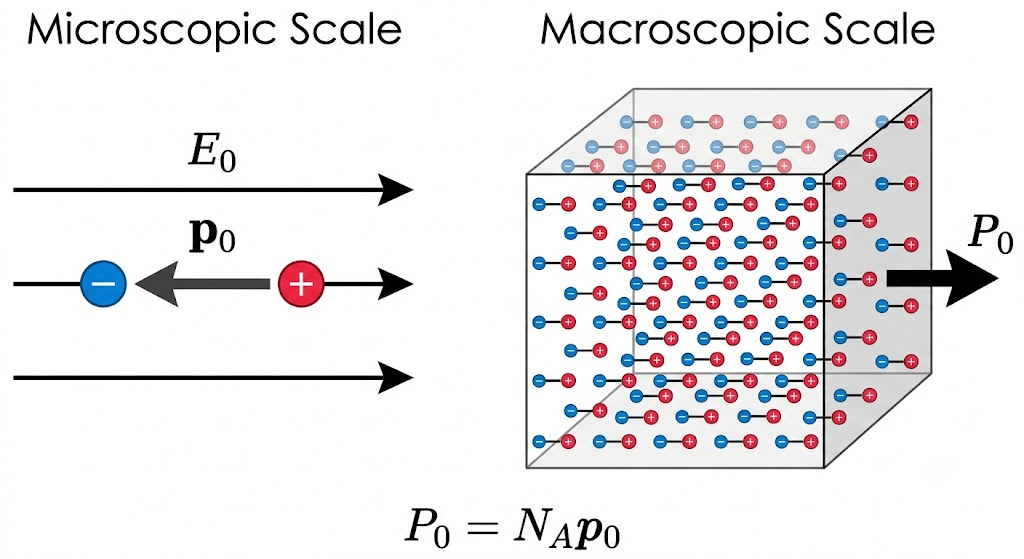
\includegraphics[width=0.6\textwidth]{Figures/Chapter 1/microscopic_to_macroscopic.jpg}
    \caption{From Microscopic to Macroscopic: Integrating $N_A$ microscopic atomic dipoles per unit volume yields the macroscopic polarization vector $\mathbf{P}$.}
\end{figure}

Ultimately, each atom's displaced electron cloud creates a tiny dipole $p_0$, and stacking $N_A$ of these per unit volume gives the macroscopic polarization $P_0 = -N_A e\,x_0$. This is the quantity that links the microscopic atomic world to Maxwell's macroscopic equations.

\subsection{Deriving the Susceptibility \texorpdfstring{$\chi(\omega)$}{χ(ω)}}

Recall from fundamental electromagnetics that macroscopic polarization is formally linked to the external electric field by a dimensionless material property called the \textbf{electric susceptibility} $\chi$:
\begin{equation*}
    P_0 = \varepsilon_0\,\chi(\omega)\,E_0,
\end{equation*}
where $\varepsilon_0$ is the permittivity of free space and $\chi(\omega)$ is a complex, frequency-dependent number that tells us exactly how strongly the material polarizes in response to the applied field at frequency $\omega$.

To find a concrete expression for $\chi(\omega)$, we equate our two definitions of $P_0$:
\begin{equation*}
    \varepsilon_0\,\chi(\omega)\,E_0 = -N_A\,e\,x_0
\end{equation*}
Substituting our explicitly derived displacement phasor $x_0 = -\dfrac{e}{m}\dfrac{E_0}{\omega_0^2 - \omega^2 + j\eta\omega}$:
\begin{equation*}
    \varepsilon_0\,\chi(\omega)\,E_0 = \frac{N_A\,e^2}{m} \frac{E_0}{\omega_0^2 - \omega^2 + j\eta\omega}
\end{equation*}
The applied field $E_0$ perfectly cancels from both sides, proving that susceptibility is an intrinsic material property independent of the light's intensity (the hallmark of linear optics). Isolating $\chi(\omega)$ yields our fundamental result:
\begin{keyresult}
    \begin{equation}
        \chi(\omega) = \frac{N_A\,e^2}{\varepsilon_0\,m}\,\frac{1}{\omega_0^2 - \omega^2 + j\eta\omega}
    \end{equation}
\end{keyresult}
Note that $\chi(\omega)$ is complex-valued — its real part will drive dispersion and its imaginary part will drive optical absorption. This expression is \emph{exact} within the classical Lorentz model (which, behaving as a damped spring, can only dissipate energy, never amplify it). Its magnitude peaks sharply at $\omega = \omega_0$, and its phase encodes whether the material's response leads or lags the driving field.

\subsubsection{The Exact \texorpdfstring{$\chi'$, $\chi''$}{χ', χ''} Spectral Profiles}

Just like we did for the microscopic displacement $x_0$, we can decompose the total complex susceptibility $\chi(\omega)$ into its purely real part ($\chi'$) and purely imaginary part ($\chi''$). To find their exact profiles, we recall the foundational bridge equation established earlier that links the macroscopic susceptibility directly to the microscopic displacement:
\begin{equation*}
    \chi = -\frac{N_A e}{\varepsilon_0 E_0} x_0
\end{equation*}

By explicitly writing both variables in their expanded complex forms ($\chi = \chi' + j\chi''$ and $x_0 = x' + jx''$), we can substitute them directly into the bridge equation:
\begin{equation*}
    \chi' + j\chi'' = -\frac{N_A e}{\varepsilon_0 E_0} (x' + jx'') \quad \Rightarrow \quad \chi' + j\chi'' = \left(-\frac{N_A e}{\varepsilon_0 E_0}x'\right) + j\left(-\frac{N_A e}{\varepsilon_0 E_0}x''\right)
\end{equation*}

For two complex equations to be mathematically equal, their purely real parts must exactly match, and their strictly imaginary parts must exactly match. Equating them directly proves that the macroscopic susceptibility components are nothing more than perfectly scaled replicas of the electron's displacement components:
\begin{equation*}
    \chi' = -\frac{N_A e}{\varepsilon_0 E_0}x' \quad \text{and} \quad \chi'' = -\frac{N_A e}{\varepsilon_0 E_0}x''
\end{equation*}

Finally, we simply substitute the exact algebraic formulas for $x'$ and $x''$ of the driven electron (which we derived earlier) into these two scaling equations. This immediately yields the exact mathematical forms for the macroscopic susceptibility profiles:
\begin{keyresult}
    \begin{gather}
        \chi'(\omega) = \frac{N_A\,e^2}{\varepsilon_0\,m} \left[ \frac{\omega_0^2 - \omega^2}{(\omega_0^2 - \omega^2)^2 + (\eta\omega)^2} \right] \quad \text{(Real Part $\to$ Controls Dispersion)} \\[1ex]
        \chi''(\omega) = -\frac{N_A\,e^2}{\varepsilon_0\,m} \left[ \frac{\eta\omega}{(\omega_0^2 - \omega^2)^2 + (\eta\omega)^2} \right] \quad \text{(Imaginary Part $\to$ Controls Absorption)}
    \end{gather}
\end{keyresult}

As expected, the macroscopic susceptibility profiles have perfectly inherited the real and imaginary mathematical structure of the single isolated electron.

\subsubsection{The Near-Resonance Approximation}

While the classical equations derived above are mathematically rigorous for a theoretical spring, applying them to a real atom across the entire spectrum is a physical mistake. In reality, this single-oscillator model only accurately captures the true behavior of real atoms within a very narrow frequency band extremely close to a specific atomic transition. Furthermore, outside of this tight window, the resonant susceptibility drops to zero and the atoms become optically invisible. Because all the relevant optical physics occurs precisely where $\omega \approx \omega_0$, we are physically justified in making a powerful mathematical simplification.

To navigate the mathematics near resonance, it is extremely useful to define a new universal parameter called the \textbf{normalised frequency detuning} $\delta$. It measures exactly how far the driving frequency $\omega$ is from the resonance $\omega_0$, scaled by the half-linewidth $\eta/2$:
\begin{equation*}
    \delta \equiv \frac{\omega - \omega_0}{\eta/2} = \frac{2(\omega - \omega_0)}{\eta}
\end{equation*}
Because both the numerator and denominator have units of frequency (rad/s), $\delta$ is completely dimensionless. It serves as a pure, unitless ``score'' of how far off-resonance the light is.

With this definition in hand, we now apply our near-resonance approximation ($\omega \approx \omega_0$) to the exact susceptibility equation. We start by factoring the $\omega_0^2 - \omega^2$ term in its denominator as a difference of squares:
\begin{equation*}
    \omega_0^2 - \omega^2 = (\omega_0 - \omega)(\omega_0 + \omega) \quad \Rightarrow \quad \omega_0^2 - \omega^2 \approx 2\omega(\omega_0 - \omega)
\end{equation*}

Substituting this approximated term back into the exact expression for $\chi(\omega)$ gives:
\begin{equation*}
    \chi(\omega) = \frac{N_A\,e^2}{\varepsilon_0\,m}\,\frac{1}{\omega_0^2 - \omega^2 + j\eta\omega} \quad \Rightarrow \quad \chi(\omega) \approx \frac{N_A\,e^2}{\varepsilon_0\,m}\,\frac{1}{2\omega(\omega_0 - \omega) + j\eta\omega}
\end{equation*}

To mathematically expose our detuning parameter, we factor out the common friction term $\eta\omega$ from the denominator:
\begin{equation*}
    \chi(\omega) \approx \frac{N_A\,e^2}{\varepsilon_0\,m\,\eta\omega} \frac{1}{\dfrac{2(\omega_0 - \omega)}{\eta} + j}
\end{equation*}

Looking at the purely real fraction that has organically emerged in the denominator, we immediately recognize it as the exact negative of our detuning factor: $\dfrac{2(\omega_0 - \omega)}{\eta} = -\delta$.

Substituting this definition into our susceptibility yields its elegant, universal near-resonance form:
\begin{equation*}
    \chi(\omega) \approx \frac{N_A\,e^2}{\varepsilon_0\,m\,\eta\omega} \frac{1}{-\delta + j}
\end{equation*}

Finally, to cleanly separate this into its purely real and purely imaginary parts ($\chi = \chi' + j\chi''$), we multiply the numerator and denominator by the complex conjugate $(-\delta - j)$:
\begin{equation*}
    \chi(\omega) \approx \frac{N_A\,e^2}{\varepsilon_0\,m\,\eta\omega} \left( \frac{1}{-\delta + j} \cdot \frac{-\delta - j}{-\delta - j} \right) \quad \Rightarrow \quad \chi(\omega) \approx \frac{N_A\,e^2}{\varepsilon_0\,m\,\eta\omega} \left( \frac{-\delta - j}{\delta^2 + 1} \right)
\end{equation*}

By cleanly splitting the fraction, we explicitly isolate the real and imaginary components:
\begin{equation*}
    \chi(\omega) \approx \frac{N_A\,e^2}{\varepsilon_0\,m\,\eta\omega} \left( \frac{-\delta}{1 + \delta^2} + j \frac{-1}{1 + \delta^2} \right)
\end{equation*}

This definitively yields the two individual functions that strictly govern how light interacts with matter near a resonance:
\begin{keyresult}
    \begin{gather}
        \chi'(\omega) \approx \frac{N_A\,e^2}{\varepsilon_0\,m\,\eta\omega}\left(\frac{-\delta}{1 + \delta^2}\right) \quad \text{(Real Part $\to$ Controls Dispersion)}\\[1ex]
        \chi''(\omega) \approx \frac{N_A\,e^2}{\varepsilon_0\,m\,\eta\omega}\left(\frac{-1}{1 + \delta^2}\right) \quad \text{(Imaginary Part $\to$ Controls Absorption)}
    \end{gather}
\end{keyresult}

\begin{keyinsight}[The Anatomy of the Lorentzian Profiles]
    Both $\chi'$ and $\chi''$ share the exact same denominator $(1 + \delta^2)$, but their different numerators completely dictate their physical behavior as you tune the laser across the resonance:
    \begin{itemize}
        \item \textbf{Exact Resonance ($\delta = 0$):} The laser perfectly matches the atomic frequency $\omega_0$. Because the numerator of $\chi'$ is exactly zero, dispersion vanishes entirely ($|\chi'| = 0$). However, the denominator $(1 + \delta^2) = 1$ is at its absolute minimum, meaning the absorption term $|\chi''|$ reaches its maximum possible peak. At exact resonance, the atom's entire response goes into absorbing energy, not bending light.
        \item \textbf{The Half-Width Points ($|\delta| = 1$):} The laser is off-resonance by exactly $\eta/2$. The denominator becomes $(1 + 1^2) = 2$, meaning absorption $|\chi''|$ has dropped to exactly half of its peak value. However, something completely different happens for dispersion! Because $\chi' \propto \frac{\delta}{1+\delta^2}$, setting $|\delta|=1$ yields $\frac{1}{2}$, which is the mathematical \emph{maximum} of this function. So exactly at the points where absorption drops to 50\%, dispersion fiercely peaks.
        \item \textbf{Far Off-Resonance ($|\delta| \gg 1$):} The mismatch is much larger than the damping rate $\eta$. The denominator $(1 + \delta^2) \approx \delta^2 \gg 1$, driving both $\chi'$ and $\chi''$ to effectively zero. As seen earlier, far from resonance the classical electron acts as either a pure spring or a pure inertial mass, and in both cases, no net energy is permanently absorbed. The large $\delta^2$ dominating the denominator is the mathematical signature of that physics.
    \end{itemize}
\end{keyinsight}

\begin{figure}[H]
    \centering
    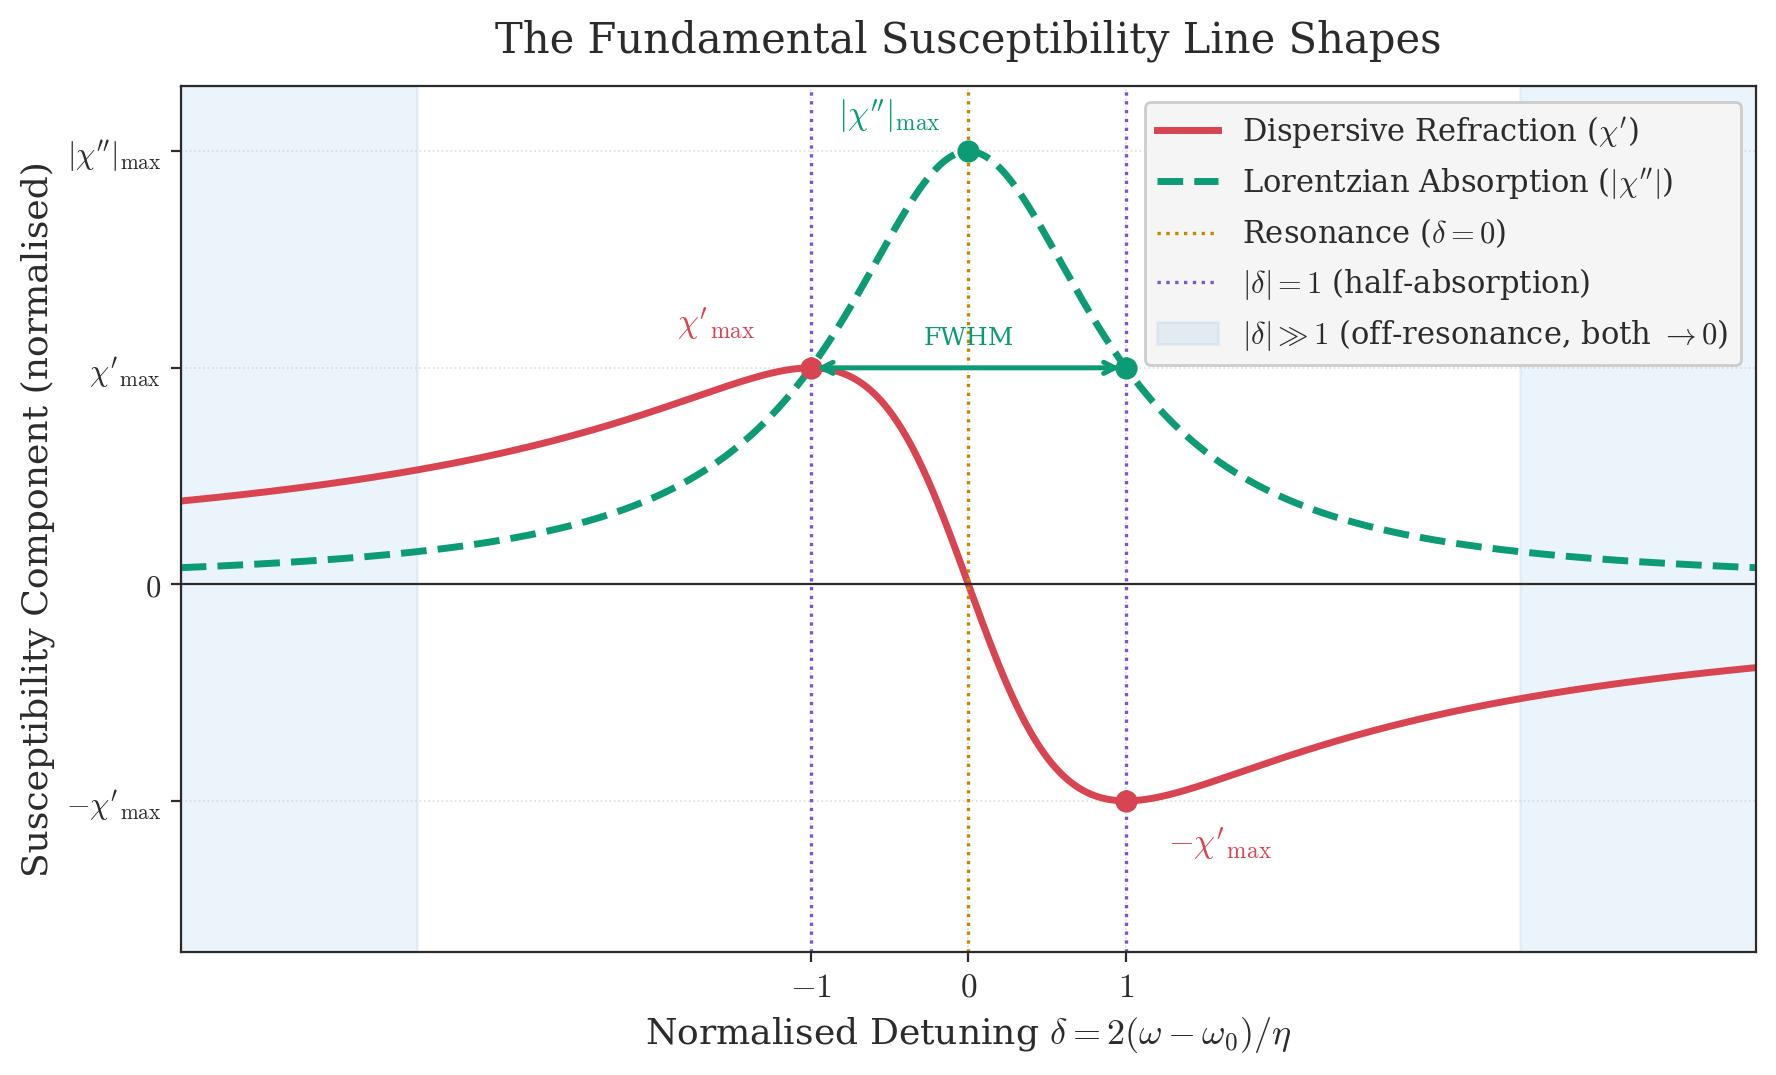
\includegraphics[width=0.65\textwidth]{Figures/Chapter 1/susceptibility_profiles.jpg}
    \caption{The Susceptibility Profiles: The dispersive real part ($\chi'$) and the Lorentzian imaginary part ($\chi''$) strictly govern refraction and absorption.}
\end{figure}

Now let's extract the physical implications embedded within the susceptibility profiles shown above. This visualization provides us with a rigorous mathematical map of the atom's optical response, simultaneously encoding the exact behaviour of both its internal friction (manifesting as absorption) and its physical inertia (manifesting as dispersion) as it interacts with the light.

Starting with the absorption peak, notice the double-headed arrow labelled FWHM. The \textbf{Full Width at Half Maximum (FWHM)} is the physical frequency span between the two points where the absorption profile drops to exactly half of its peak value.

To calculate this span, we first find where the normalized Lorentzian absorption drops to 50\%:
\begin{equation*}
    \frac{1}{1 + \delta^2} = \frac{1}{2} \quad \Rightarrow \quad 1 + \delta^2 = 2 \quad \Rightarrow \quad \delta = \pm 1
\end{equation*}

This tells us that the absorption drops to half its maximum at two specific dimensionless detunings: $\delta = +1$ and $\delta = -1$. To convert these coordinates back into physical frequencies, we simply rearrange our detuning definition to solve for $\omega$:
\begin{equation*}
    \delta = \frac{2(\omega - \omega_0)}{\eta} \quad \Rightarrow \quad \omega = \omega_0 + \frac{\eta}{2}\delta
\end{equation*}

Plugging in our two half-maximum points ($\delta = \pm 1$), the exact physical frequencies where the absorption drops to 50\% are:
\begin{equation*}
    \omega_1 = \omega_0 - \frac{\eta}{2} \quad \text{and} \quad \omega_2 = \omega_0 + \frac{\eta}{2}
\end{equation*}

The FWHM is simply the difference between these two boundary frequencies ($\Delta\omega_{\text{FWHM}} = \omega_2 - \omega_1$). Subtracting them immediately yields a profound mathematical result:
\begin{equation*}
    \Delta\omega_{\text{FWHM}} = \left( \omega_0 + \frac{\eta}{2} \right) - \left( \omega_0 - \frac{\eta}{2} \right) \quad \Rightarrow \quad \Delta\omega_{\text{FWHM}} = \eta
\end{equation*}

Before we interpret this physically, a practical note is required. We have worked exclusively in angular frequency $\omega$ (rad/s), which is the natural language of the mathematics. However, optical bandwidth in any real laboratory is measured in ordinary frequency $\nu$ (Hz). Because $\omega = 2\pi\nu$, the frequency width $\Delta\nu_{\text{FWHM}}$ is found by simply dividing by $2\pi$:
\begin{equation*}
    \Delta\nu_{\text{FWHM}} = \frac{\Delta\omega_{\text{FWHM}}}{2\pi} = \frac{\eta}{2\pi}
\end{equation*}

We collect both of these extremely important forms into a single definitive summary:

\begin{keyresult}
    \begin{gather}
        \Delta\omega_{\text{FWHM}} = \eta \nonumber \\[1ex]
        \Delta\nu_{\text{FWHM}} = \frac{\eta}{2\pi}
    \end{gather}
\end{keyresult}

This derivation achieves something beautiful: it bridges the microscopic math to the macroscopic reality. A physical system with higher internal friction ($\eta$) naturally restricts the electron's ability to sustain a long, ringing oscillation, causing its excited energy to decay much more rapidly. In the frequency domain, this faster time decay translates directly into a broader, more smeared-out resonance bandwidth. By proving that the FWHM is mathematically identical to $\eta$ (or $\eta/2\pi$ in Hz), we have taken an abstract friction coefficient from a microscopic differential equation and revealed it to be exactly the macroscopic, measurable spectral width of the light that you would see on a laboratory spectrum analyser.

\begin{keyinsight}[Why Dispersion Flips but Absorption is Symmetrical]
    Re-examining the susceptibility profiles plotted earlier, notice that the absorption curve ($\chi''$, the dashed line) is perfectly symmetric around $\delta = 0$. Mathematically, its denominator $(1+\delta^2)$ squares the detuning, erasing the sign. Physically, the atom doesn't care if you drive it too fast ($\delta > 0$) or too slow ($\delta < 0$) — either way, you are off-rhythm, and energy transfer drops symmetrically.

    Dispersion ($\chi'$, the solid line), however, is wildly asymmetric — it is positive for negative detuning, crosses zero at resonance, and dips negative for positive detuning. Why? Because of the uncanceled $\delta$ in its numerator!
    \begin{itemize}
        \item \textbf{Negative Detuning ($\delta < 0$, $\omega < \omega_0$):} We are driving the electron slowly. As we saw in the low-frequency limit, it acts like a pure spring and moves \emph{in-phase} with the light. This in-phase electron movement adds constructively to the light wave, effectively making the material feel ``denser'' and \textbf{slowing the light down} (positive dispersion).
        \item \textbf{Positive Detuning ($\delta > 0$, $\omega > \omega_0$):} We are driving the electron too quickly. As we saw in the high-frequency limit, its inertia prevents it from keeping up, and its position flips to $180^\circ$ \emph{out-of-phase}. This completely opposite movement destructively interferes with the light wave, making the material feel ``less dense'' and causing the phase velocity to \textbf{speed up} (negative dispersion).
    \end{itemize}
    This beautifully illustrates how microscopic electron inertia is directly responsible for macroscopic phenomena like light slowing down in glass!
\end{keyinsight}

\begin{keyinsight}[Kramers-Kronig Relations]
    Notice how $\chi'$ and $\chi''$ are intrinsically linked — they share the exact same denominator $(1 + \delta^2)$. This is not a coincidence. Because causation must precede effect (the causality principle), the dispersive and absorptive responses of any linear, causal medium are never independent: they are rigorously locked together via integral transforms known as the \textbf{Kramers-Kronig relations}. Knowing the absorption profile $\chi''(\omega)$ at all frequencies is sufficient to uniquely reconstruct the dispersion profile $\chi'(\omega)$, and vice versa. Physically, this means a material cannot absorb light without also bending it — dispersion and absorption are two inseparable facets of the same underlying causal response.
\end{keyinsight}

\subsection{Relative Permittivity and the Complex Refractive Index}

In every real optoelectronic device, there are \textit{two} optically distinct populations of atoms that we must account for simultaneously:

\begin{enumerate}
    \item \textbf{The host medium.} This is the passive, transparent bulk material — silica glass in an optical fibre, a YAG crystal in a solid-state laser, or even just a background gas in a vapour cell. The host has its own refractive index $n_b$ (the subscript $b$ stands for ``background''), which is real, large, and essentially constant across the narrow frequency ranges we care about. It does not absorb at our operating frequency.
    \item \textbf{The transition atoms.} These are the optically active species embedded inside the host — Er$^{3+}$ ions in a silica fibre, Nd$^{3+}$ ions in a YAG crystal, and so on. They are a tiny minority compared to the host atoms, but they are the only ones doing anything interesting: they absorb and shift the phase of the wave via their dipole resonance. Their contribution to the susceptibility is small, complex, and strongly frequency-dependent.
\end{enumerate}

Every subsequent derivation relies explicitly on this physical split. The host medium establishes a large, purely real background, while the transition atoms introduce a small, complex, and highly resonant correction.

With this foundation in place, we can now define the exact quantity that bridges the microscopic atomic susceptibility to the macroscopic propagation of the wave.

\subsubsection{From Susceptibility to Permittivity}

Recall from Maxwell's equations that the electric displacement field $\mathbf{D}$ is related to the applied electric field $\mathbf{E}$ and the total macroscopic polarisation $\mathbf{P}$ of the medium by:
\begin{equation*}
    \mathbf{D} = \varepsilon_0 \mathbf{E} + \mathbf{P},
\end{equation*}
where:
\begin{itemize}
    \item $\mathbf{D}$: the electric displacement field — the ``total'' field including the medium's response.
    \item $\varepsilon_0$: the permittivity of free space.
    \item $\mathbf{P}$: the macroscopic polarisation — the dipole moment per unit volume induced in the medium.
\end{itemize}

In a linear medium, the total polarisation $\mathbf{P}$ is driven by the electric field via the total electric susceptibility $\chi_{\text{total}}$:
\begin{equation*}
    \mathbf{P} = \varepsilon_0 \chi_{\text{total}} \mathbf{E},
\end{equation*}
where $\chi_{\text{total}}$ is dimensionless and complex. Substituting this back into the expression for $\mathbf{D}$ yields:
\begin{equation*}
    \mathbf{D} = \varepsilon_0 \mathbf{E} + \varepsilon_0 \chi_{\text{total}} \mathbf{E} = \varepsilon_0(1 + \chi_{\text{total}})\mathbf{E}.
\end{equation*}

We now define the \textbf{relative permittivity} $\varepsilon_r$ (often called the \textbf{dielectric constant}) as precisely the complex factor relating $\mathbf{D}$ directly to $\varepsilon_0 \mathbf{E}$:
\begin{equation*}
    \varepsilon_r = 1 + \chi_{\text{total}},
\end{equation*}
so that $\mathbf{D} = \varepsilon_0 \varepsilon_r \mathbf{E}$. This single complex number encodes absolutely everything the composite material does to an electromagnetic wave — its real part dictates the phase velocity, and its imaginary part dictates the absorption.

Because the host and the transition atoms respond independently to the light, their individual susceptibilities simply add together to form the total response:
\begin{equation*}
    \chi_{\text{total}} = \chi_{\text{host}} + \chi_{\text{transition}},
\end{equation*}
and therefore, the total relative permittivity of the device is:
\begin{equation*}
    \varepsilon_r = 1 + \chi_{\text{host}} + \chi_{\text{transition}}.
\end{equation*}

Now we apply two key physical facts about the host that let us simplify this immediately.

\textbf{Fact 1 — The host is lossless at our operating frequency.} Since the host is transparent, it has no absorption, which means its susceptibility is purely real:
\begin{equation*}
    \chi''_{\text{host}} = 0 \quad \Rightarrow \quad \chi_{\text{host}} \in \mathbb{R}.
\end{equation*}
The host shifts the phase of the wave (it has a refractive index), but it does not attenuate it.

\textbf{Fact 2 — The pure host material has a well-defined refractive index $n_b$.} If the active transition atoms were completely removed, the remaining pure host medium would have its own standalone relative permittivity, $\varepsilon_{r,\text{host}} = 1 + \chi_{\text{host}}$. By the fundamental relationship between permittivity and refractive index ($\varepsilon_r = n^2$), this baseline permittivity must exactly equal the square of the host's refractive index $n_b$:
\begin{equation*}
    \varepsilon_{r,\text{host}} = 1 + \chi_{\text{host}} = n_b^2,
\end{equation*}
This is simply the standard refractive index you would look up in a datasheet for the bulk host material, ignoring the active dopant atoms entirely.

We can now substitute this baseline host response directly back into our equation for the total permittivity:
\begin{equation*}
    \varepsilon_r = \underbrace{1 + \chi_{\text{host}}}_{n_b^2} + \chi_{\text{transition}}.
\end{equation*}

From this point forward, we will write $\chi$ to mean $\chi_{\text{transition}}$ exclusively — the small, complex, resonant susceptibility of the active atoms only. With that convention, the full expression collapses to:

\begin{keyresult}
    \begin{equation}
        \varepsilon_r = n_b^2 + \chi
    \end{equation}
\end{keyresult}
Where:
\begin{itemize}
    \item $n_b^2$: The \textbf{host background} contribution — real, large, non-resonant. It sets the baseline refractive index that the wave ``sees'' even when the active atoms are completely inactive.
    \item $\chi = \chi' + j\chi''$: The \textbf{transition atoms'} contribution — small, complex, and strongly resonant. Specifically, $\chi'$ dictates dispersion (a frequency-dependent shift in phase velocity), while $\chi''$ dictates absorption.
\end{itemize}

\subsubsection{Deriving the Complex Refractive Index \texorpdfstring{$\tilde{n}$}{ñ}}

Because the total relative permittivity $\varepsilon_r = n_b^2 + \chi$ is complex, the refractive index of the composite material must also be complex. We therefore define the \textbf{complex refractive index} $\tilde{n}$ precisely as the quantity whose square equals the total permittivity:
\begin{equation*}
    \tilde{n}^2 = \varepsilon_r = n_b^2 + \chi, \qquad \tilde{n} = n + j\kappa,
\end{equation*}
where:
\begin{itemize}
    \item $n$: the real refractive index. It determines how fast the wave's phase propagates through the medium (phase velocity is $c_0/n$).
    \item $\kappa$: the \textbf{extinction coefficient}. It determines how quickly the wave's amplitude decays as it propagates.
\end{itemize}

Our goal now is to isolate $n$ and $\kappa$ individually in terms of quantities we already know: $n_b$, $\chi'$, and $\chi''$. We start by relating them through the square root of the relative permittivity:
\begin{equation*}
    \tilde{n} = \sqrt{\varepsilon_r} = \sqrt{n_b^2 + \chi}
\end{equation*}

By factoring out $n_b^2$, we can expose a dimensionless ratio inside the square root:
\begin{equation*}
    \tilde{n} = \sqrt{n_b^2\!\left(1 + \frac{\chi}{n_b^2}\right)} = n_b\sqrt{1 + \frac{\chi}{n_b^2}}
\end{equation*}

To simplify the square root, we apply the binomial approximation $(1+x)^{1/2} \approx 1 + x/2$. This mathematical expansion is only valid when the second term is very small ($|x| \ll 1$), which in our equation requires that $|\chi| \ll n_b^2$. Fortunately, this is not just a convenient assumption—it is a physical guarantee in optoelectronic devices.

\begin{keyinsight}[Why the Transition Atom Contribution is Always Small]
    Because the active transition atoms are typically a \textit{dilute dopant} within a dense host medium, their number density is extremely low. Since macroscopic susceptibility scales directly with density, these sparse dopants produce only a tiny perturbation ($\chi$) atop the host's massive baseline permittivity ($n_b^2$). Thus, the condition $|\chi| \ll n_b^2$ is physically guaranteed.
\end{keyinsight}

Because the condition securely holds, we substitute $x = \chi / n_b^2$ into the binomial expansion:
\begin{equation*}
    \tilde{n} \approx n_b\!\left(1 + \frac{\chi}{2n_b^2}\right) = n_b + \frac{\chi}{2n_b}
\end{equation*}

Finally, substituting the complex formulation $\chi = \chi' + j\chi''$ explicitly separates the expression into purely real and imaginary components:
\begin{equation*}
    \tilde{n} \approx n_b + \frac{\chi' + j\chi''}{2n_b} = \left(n_b + \frac{\chi'}{2n_b}\right) + j\left(\frac{\chi''}{2n_b}\right)
\end{equation*}

Matching this directly against our definition $\tilde{n} = n + j\kappa$, we can read off the equations for the real refractive index and the extinction coefficient:

\begin{keyresult}
    \begin{gather}
        n      \approx n_b + \frac{\chi'}{2n_b} \\[1ex]
        \kappa \approx \frac{\chi''}{2n_b}
    \end{gather}
\end{keyresult}

We can notice that if the transition atoms are switched off entirely ($\chi = 0$), then $n \to n_b$ and $\kappa \to 0$: the wave propagates through the host with no attenuation, exactly as expected.

\section{Wave Propagation: Attenuation and Dispersion}


\subsection{Power Attenuation and the Absorption Coefficient \texorpdfstring{$\alpha$}{α}}

Recall that a plane wave propagating in the $+z$ direction through a medium with complex refractive index $\tilde{n}$ has the form:
\begin{equation*}
    E(z) = E_0\,e^{-j\tilde{n}\,k_0\,z} = E_0\,e^{-j(n + j\kappa)\,k_0\,z} = E_0\,e^{-jn\,k_0\,z}\cdot e^{\kappa\,k_0\,z},
\end{equation*}
where $k_0 = 2\pi/\lambda_0$ is the free-space wavenumber and $\lambda_0$ is the free-space wavelength.

The first exponential $e^{-jnk_0z}$ is the oscillating phase term — it describes the wave's spatial oscillation as it travels. The second exponential $e^{\kappa k_0 z}$ is a real amplitude term. Because $\chi''$ is inherently negative, $\kappa$ is also negative, meaning this factor causes the amplitude to decay with $z$.

The optical power (intensity) is proportional to $|E|^2$, so:
\begin{equation*}
    P(z) \propto |E(z)|^2 \propto e^{2\kappa\,k_0\,z}.
\end{equation*}
We define the \textbf{power attenuation coefficient} $\alpha$ so that power decays (or grows) as:
\begin{equation*}
    P(z) = P(0)\,e^{-\alpha z}.
\end{equation*}
Comparing the two expressions:
\begin{equation*}
    e^{-\alpha z} = e^{2\kappa\,k_0\,z} \quad \Rightarrow \quad \alpha = -2k_0\kappa.
\end{equation*}
Substitute our expression $\kappa = \chi''/(2n_b)$:
\begin{equation*}
    \alpha = -2k_0 \cdot \frac{\chi''}{2n_b}.
\end{equation*}
The factor of 2 cancels exactly:
\begin{keyresult}
    \begin{equation}
        \alpha = -\frac{k_0}{n_b}\,\chi''.
    \end{equation}
\end{keyresult}

In general optical theory, the sign of $\alpha$ dictates the fate of the wave's power:
\begin{itemize}
    \item $\alpha > 0$: The power shrinks exponentially with distance — \textbf{attenuation (loss)}.
    \item $\alpha < 0$: The power grows exponentially with distance — \textbf{amplification (gain)}.
\end{itemize}

However, in our Classical Electron Oscillator (CEO) model, the atoms are purely passive; they can only drain energy from the wave via internal friction. Because of this, the classical susceptibility $\chi''$ is inherently negative everywhere across the spectrum. Consequently, the formula $\alpha = -\frac{k_0}{n_b}\chi''$ guarantees a strictly positive $\alpha$. In a classical medium, amplification is impossible, and $\alpha$ acts exclusively as an attenuation factor.

\subsection{Normal vs.\ Anomalous Dispersion}

Away from any resonance, the real refractive index $n$ increases as the optical frequency $\omega$ increases. This is the well-known behavior called \textbf{Normal Dispersion} — it is why a prism separates white light into a rainbow, with blue (higher $\omega$) bending more than red (lower $\omega$).

However, very close to the resonance frequency $\omega_0$, something unusual happens. The real part $\chi'$ (which controls $n$) has a characteristic dispersive profile that actually \emph{dips} near $\omega_0$. In a narrow band around resonance, the refractive index $n$ \textbf{decreases} as $\omega$ increases. This phenomenon is called \textbf{Anomalous Dispersion}.

\begin{figure}[H]
    \centering
    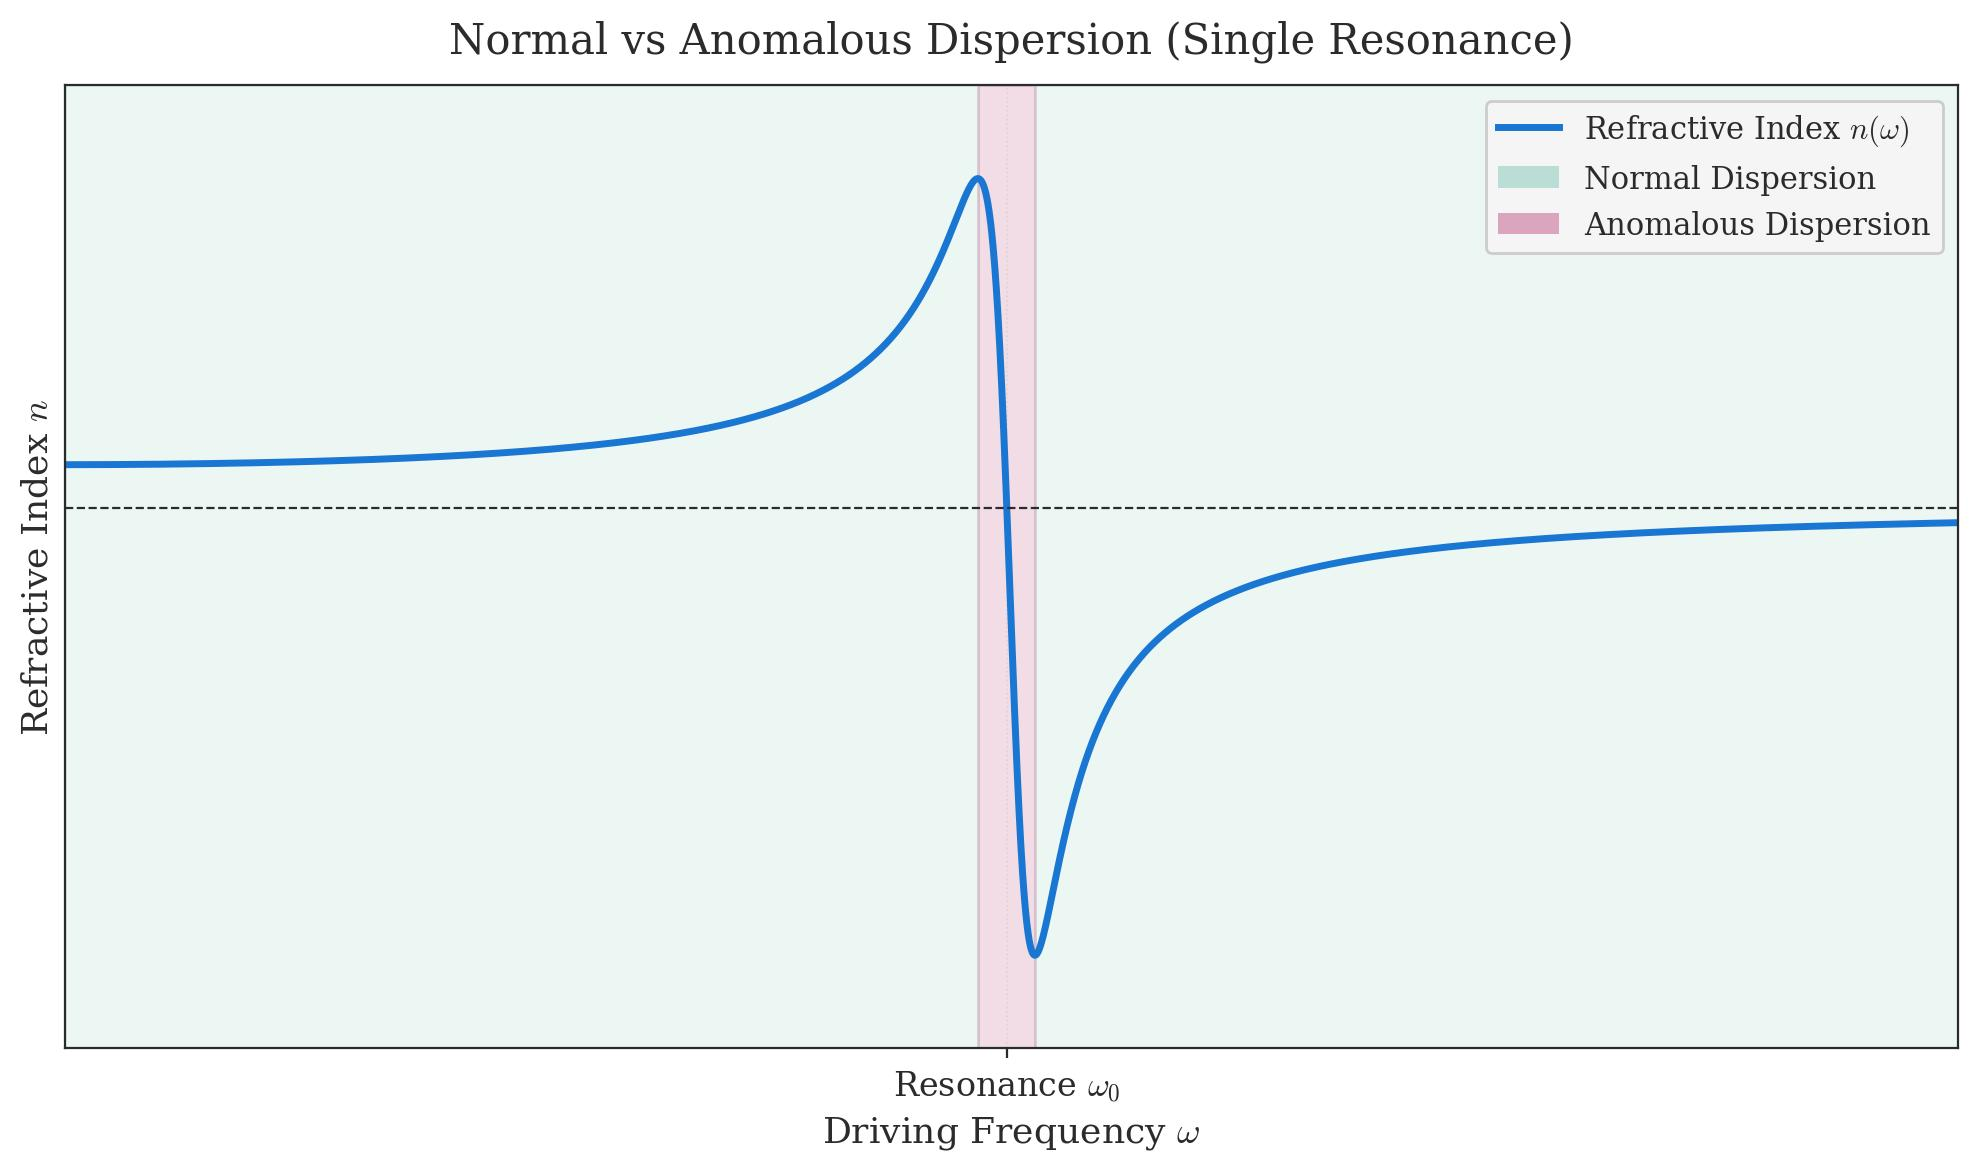
\includegraphics[width=0.65\textwidth]{Figures/Chapter 1/anomalous_dispersion_single.jpg}
    \caption{Normal vs Anomalous Dispersion (Single Resonance): The localized anomalous dispersion dip temporarily interrupts the fundamental trend of normal dispersion.}
\end{figure}

\begin{keyinsight}[The Mathematical Origins of Dispersion]
    We have derived that the refractive index tracks the real susceptibility: $n \approx n_b + \frac{\chi'}{2n_b}$.

    If we look at the full CEO susceptibility formula: $\chi(\omega) = \frac{N_A e^2}{\varepsilon_0 m}\frac{1}{\omega_0^2-\omega^2+j\eta\omega}$, we can understand \textbf{normal dispersion}. For frequencies far below resonance, the real part is dominated by the $\omega_0^2 - \omega^2$ term in the denominator. As $\omega$ increases, this denominator shrinks, causing $\chi'$ (and therefore $n$) to steadily \emph{increase}. This confirms the fundamental trend of normal dispersion.

    However, to see what happens exactly \emph{at} resonance, we switch to our specialized near-resonance approximation: $\chi' \approx \frac{N_A e^2}{\varepsilon_0 m \eta\omega}\left(\frac{-\delta}{1+\delta^2}\right)$. Because the normalized detuning $\delta$ sweeps from negative to positive as we cross $\omega_0$, the crucial $-\delta$ term in the numerator forces $\chi'$ to crash steeply downward. This localized, sharp drop in $\chi'$ translates directly into a drop in $n$, mathematically proving the existence of \textbf{anomalous dispersion}.
\end{keyinsight}

\subsection{Multiple Resonances and the Broadband Refractive Index}

Our initial classical derivations exclusively modelled a single, isolated resonance at $\omega_0$. In real materials, atoms and molecules have many different resonance frequencies — some in the infrared (IR), some in the visible, and some in the ultraviolet (UV). Each resonance produces its own localised absorption peak and its own anomalous dispersion dip.

As we sweep across the entire electromagnetic spectrum, the refractive index $n$ shows a staircase-like pattern: it climbs gradually (normal dispersion) between resonances and briefly dips (anomalous dispersion) whenever it crosses through a resonance. This broadband behavior explains why real glass has a smoothly varying $n(\lambda)$ curve across the visible range — it is in a normal-dispersion region between the nearest IR and UV resonances.

\begin{figure}[H]
    \centering
    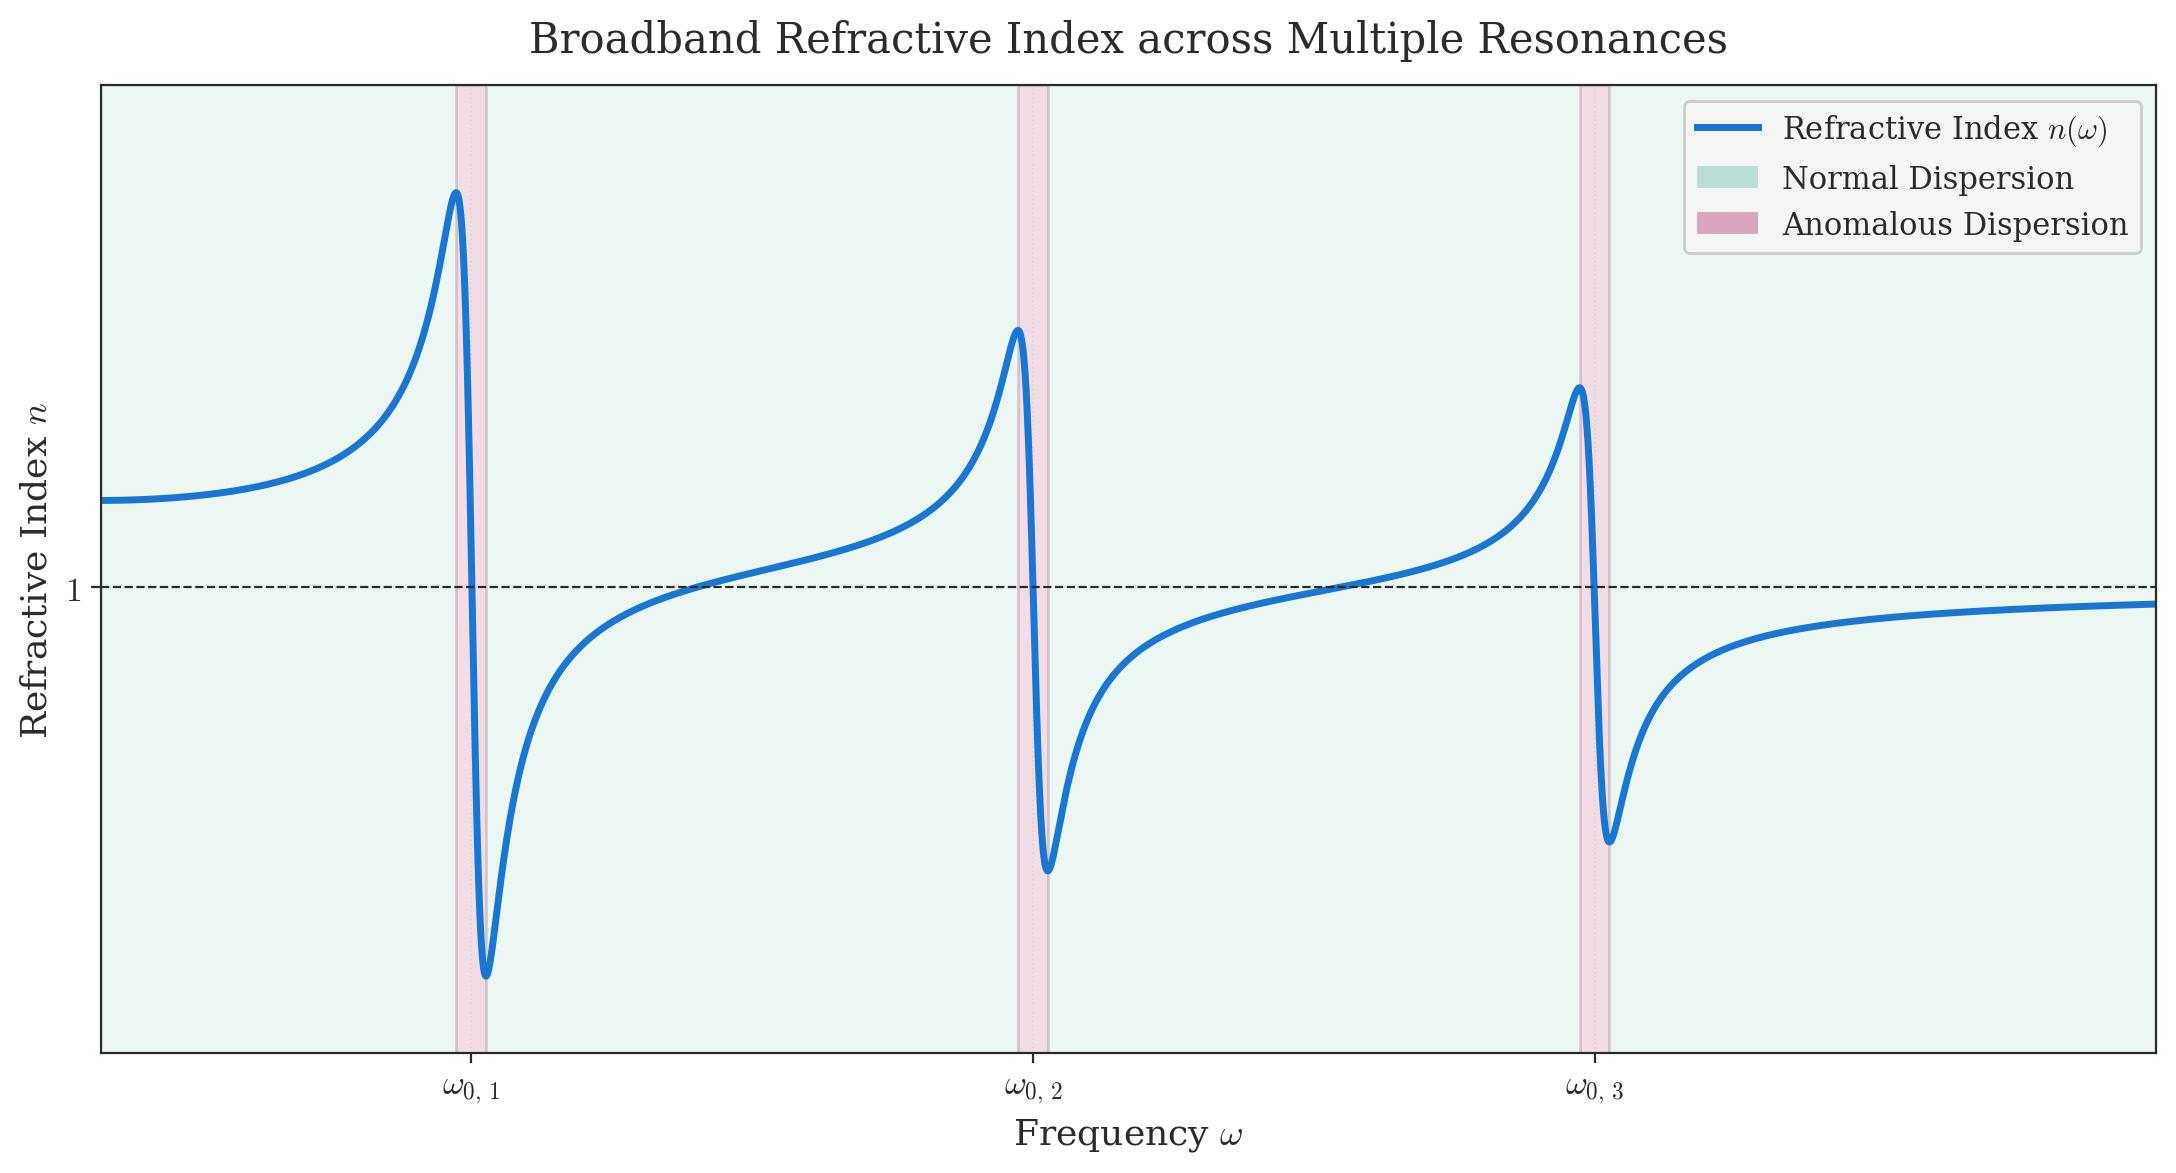
\includegraphics[width=0.75\textwidth]{Figures/Chapter 1/broadband_refractive_index.jpg}
    \caption{Broadband Refractive Index: Normal dispersion occurs between resonance peaks, while localized anomalous dispersion sharply dips exactly at each atomic resonance.}
\end{figure}

\section{The Line Shape Function}

\subsection{Motivation: What Happens to Light Passing Through Matter?}

Imagine shining a broadband white-light source directly into a block of material or a chamber of gas. What emerges on the other side?

If we shine this emerging light through a prism, it disperses into the continuous visible spectrum — from red at one end to violet at the other. But fundamentally, each distinct color simply represents a distinct driving frequency $\nu$. The material treats every single color (frequency) completely differently.

For the vast majority of frequencies, the incoming photons do not possess the exact energy required to be permanently captured. They might slightly jiggle the electron clouds as they pass (which macroscopically gives rise to phase delay and the real refractive index $n$), but they are ultimately scattered forward and emerge on the other side. This baseline behavior is \textbf{transmission}.

However, at certain highly specific frequencies, the material behaves entirely differently. According to quantum mechanics, every atom possesses a distinct, quantized ladder of allowed energy levels. If an incoming photon carries a packet of energy that \emph{exactly} matches the gap between a lower level ($E_1$) and an empty upper level ($E_2$), it is completely annihilated. Its energy is permanently absorbed, promoting the electron into the higher excited state. This resonant condition is governed by the Planck-Einstein relation,
\begin{equation*}
    E_{\text{photon}} = \Delta E = E_2 - E_1 = h\nu_0,
\end{equation*}
where $h$ is Planck's constant, and $\nu_0$ is the fundamental resonance frequency required to trigger the jump.

Because these specific photons are destroyed, their corresponding colors vanish from the transmitted beam. If you observe the emerging light through our prism, the bright, continuous rainbow will be interrupted by narrow, dark shadows (much like the famous Fraunhofer lines in the solar spectrum). These missing frequencies are what we define as the material's \textbf{absorption lines}.

\begin{keyinsight}[Multiple Transitions Mean Multiple Lines]
    Real atoms and molecules are complex. They do not have just two energy levels; they have dozens or hundreds, creating a vast ladder of possible states. Consequently, a photon can be absorbed not just from level $1\to2$, but perhaps $1\to3$, $2\to4$, or $3\to5$. Every single unique allowed transition gap ($\Delta E$) produces its own unique resonance frequency ($\nu_0$). Because of this, the output spectrum of a real material will feature a unique ``fingerprint'' of multiple distinct absorption lines, each corresponding to a specific internal quantum jump.
\end{keyinsight}

If we take this idealized quantum picture at face value, the transmission spectrum seems conceptually straightforward: a flat baseline punctuated by infinitely thin, perfectly vertical dark dips exactly at the atomic resonances $\nu_0$. However, as we are about to rigorously discover, this highly simplified picture is physically impossible. Atomic energy transitions are never perfectly sharp; they must inherently occupy a continuous, finite spectral bandwidth.

\subsection{The Absorption Line Is Not a Delta Function}

As the actual transmission spectrum below visually confirms, real absorption dips do not manifest as the perfectly vertical mathematical spikes—Dirac delta functions, $\delta(\nu - \nu_0)$—predicted by the purely idealized model. Instead, they form smooth, broadened curves.

\begin{figure}[H]
    \centering
    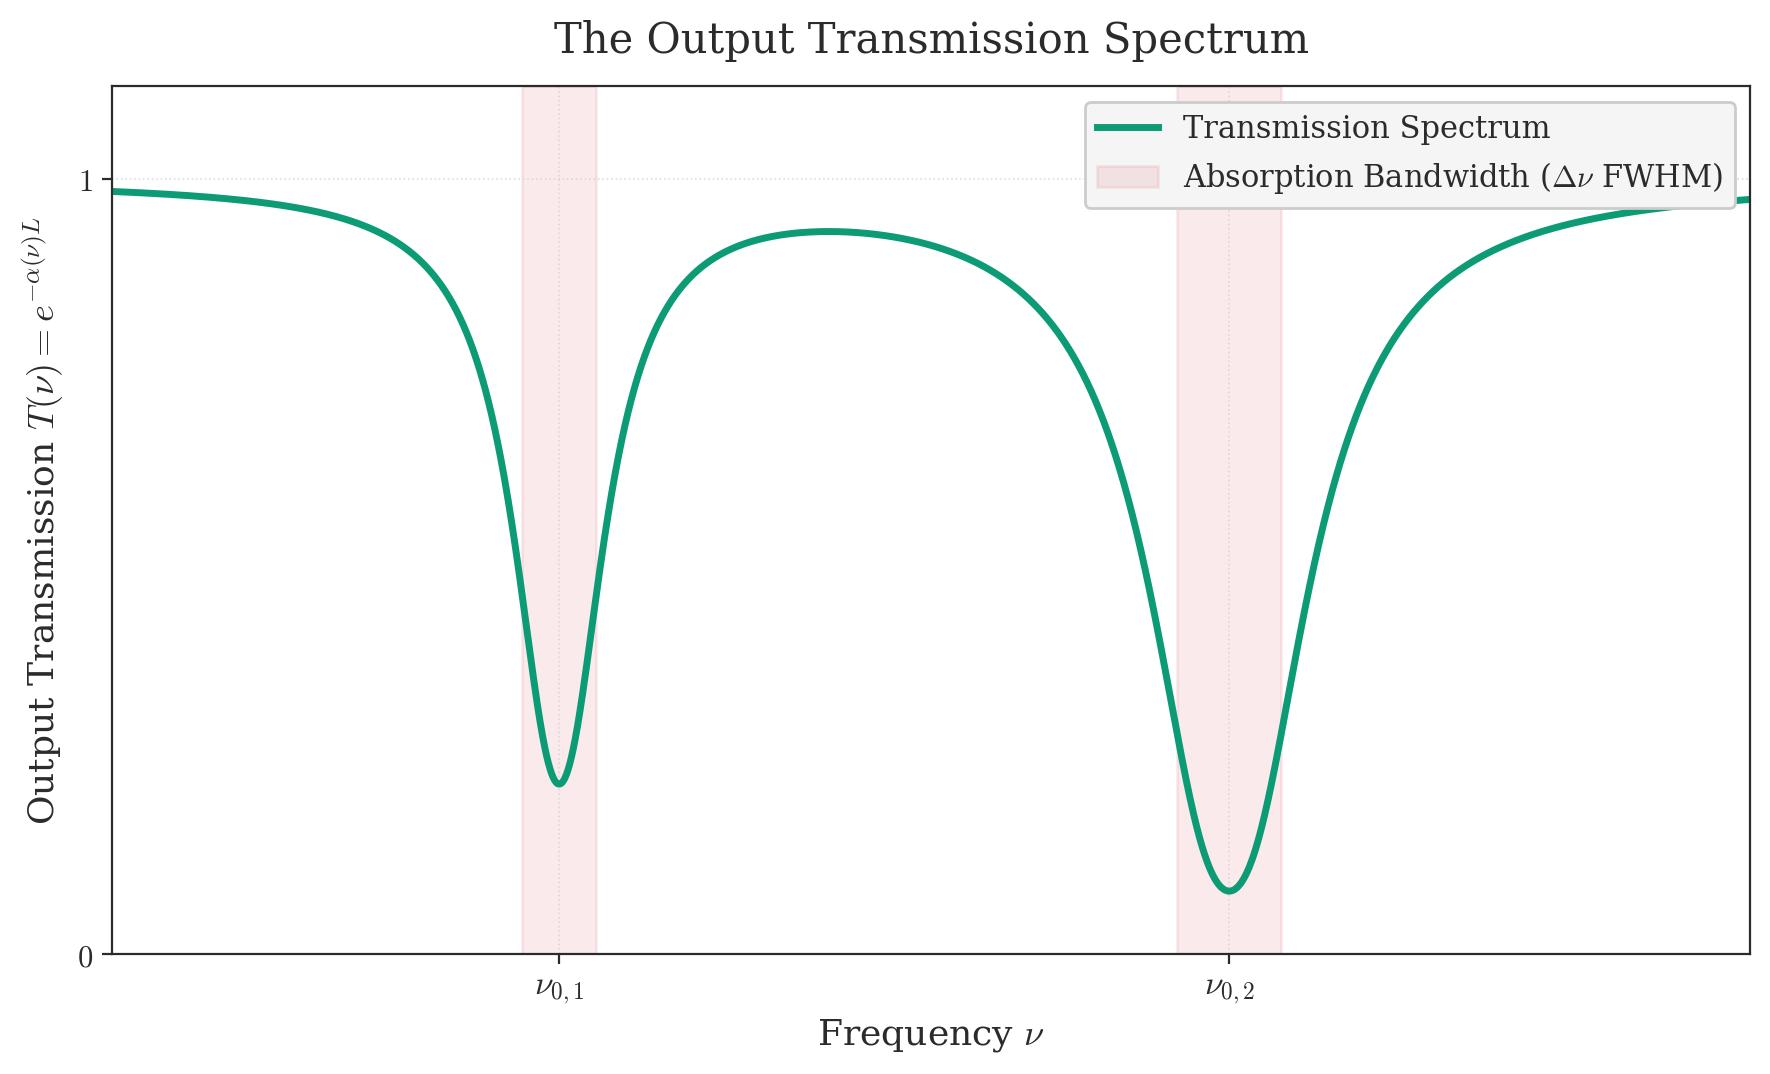
\includegraphics[width=0.65\textwidth]{Figures/Chapter 1/output_transmission_spectrum.jpg}
    \caption{The Output Transmission Spectrum: Real absorption lines are not infinitely sharp Dirac delta functions. Instead, they form broadened dips that span a finite frequency bandwidth around each resonance.}
\end{figure}

Since physical absorption clearly occupies a continuous bandwidth rather than occurring exclusively at $\nu_0$, what exactly forces reality to diverge from the Dirac delta ideal? What causes this inherent broadening?

Fundamentally, any real oscillating system experiences damping ($\eta$), which inherently broadens the resonance response. In the quantum picture, atomic energy levels are never perfectly sharp; they possess an intrinsic energy spread dictated by the excited state's finite lifetime via the Heisenberg Uncertainty Principle.

Consequently, if a photon arrives with a frequency $\nu$ slightly off $\nu_0$, the transition can still occur provided $\nu$ falls within this broadened bandwidth. While maximum absorption remains strictly at resonance, a non-zero probability of absorption persists throughout the immediate neighbourhood.

\begin{figure}[H]
    \centering
    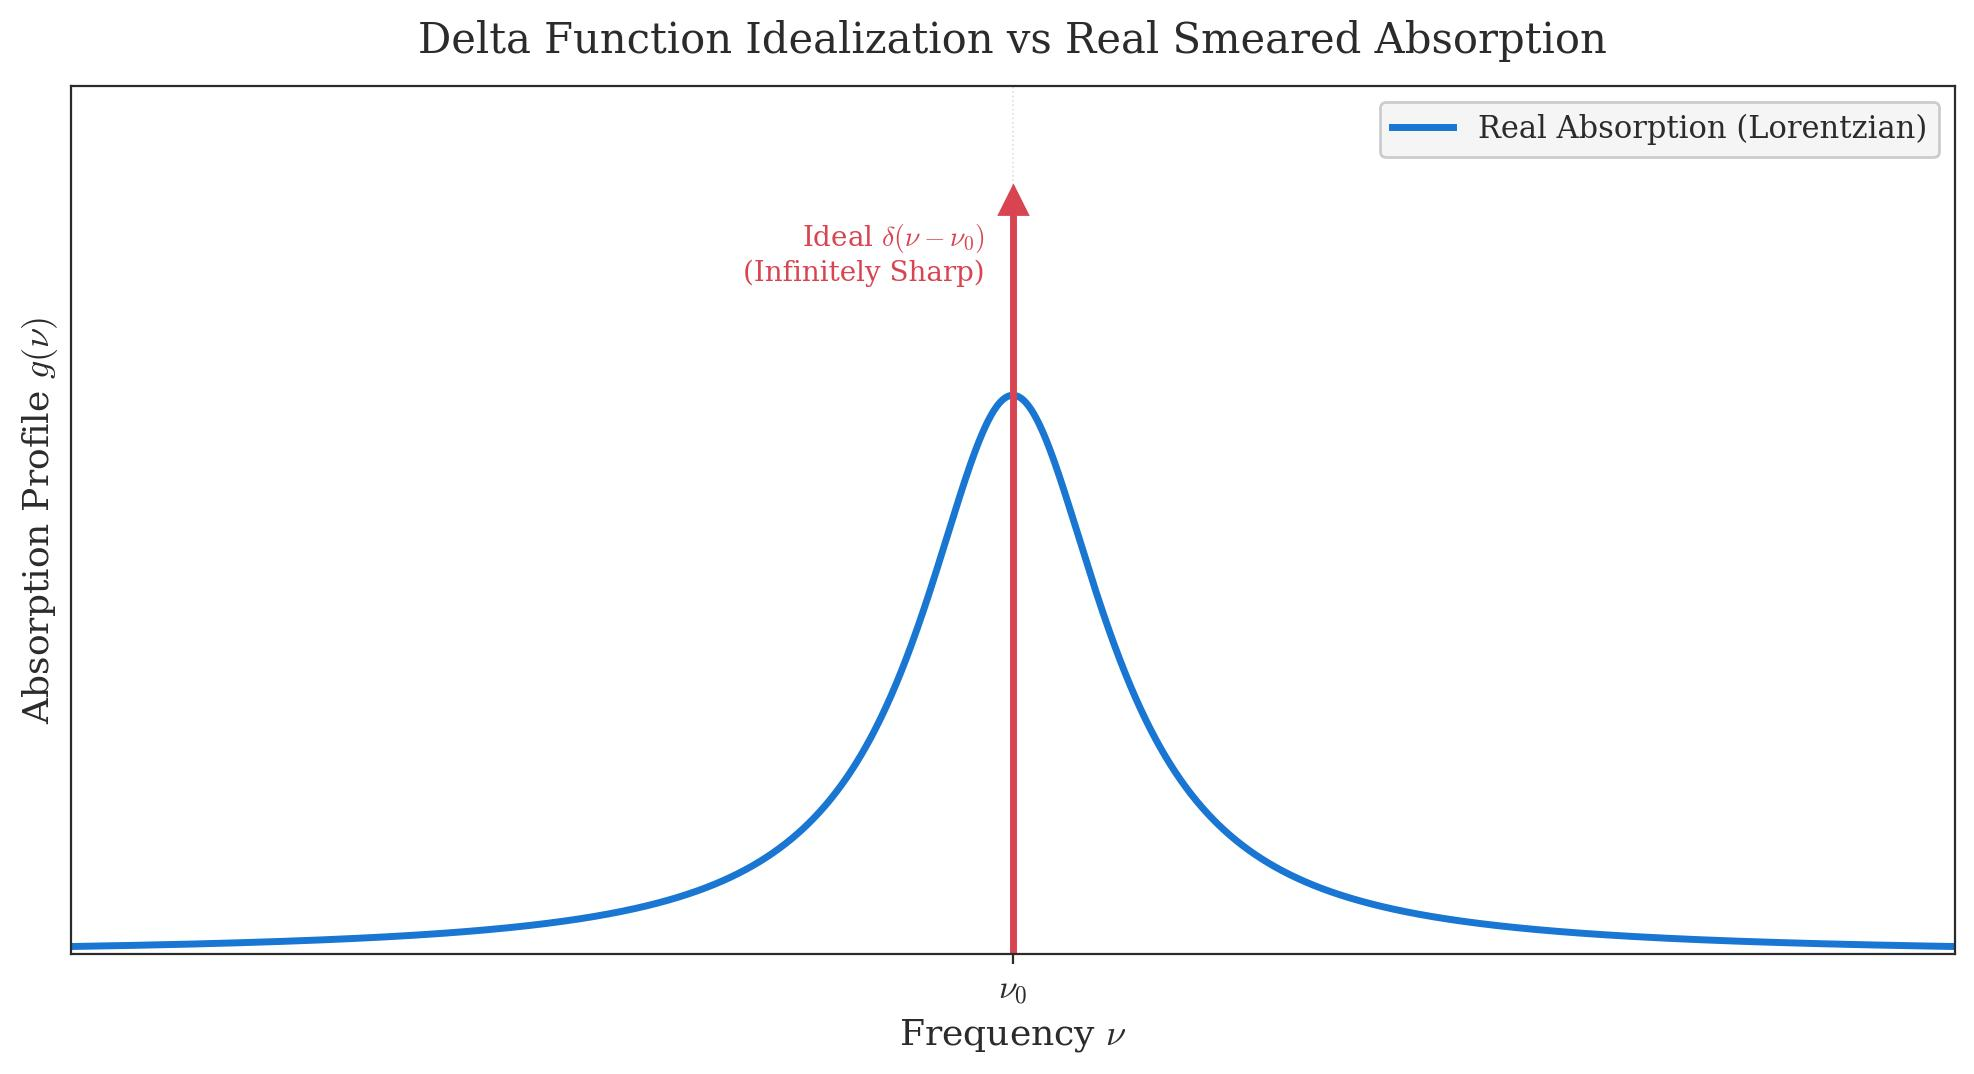
\includegraphics[width=0.65\textwidth]{Figures/Chapter 1/delta_vs_real_absorption.jpg}
    \caption{Delta Function vs. Real Absorption: Mathematical idealisation of an infinitely sharp line compared to the physically smeared Lorentzian bandwidth.}
\end{figure}

To model this smeared probability mathematically, we define the \textbf{line shape function} $g_{\nu_0}(\nu)$ — a continuous probability density representing the chance that a photon of frequency $\nu$ will be absorbed by an atomic transition centred at resonance frequency $\nu_0$. Because $g_{\nu_0}(\nu)$ is a true probability density function, the total area under the curve must equal exactly 1.

\subsection{Deriving the Line Shape Function and the Final Form of \texorpdfstring{$\alpha$}{α}}

Our goal is to transform the absorption coefficient $\alpha$ from a dense theoretical expression into a clean, practical formula. The central physical insight is that $\alpha$ must be completely separable into two independent components: its overall ``strength'' and its statistical ``shape''.
\begin{equation*}
    \alpha = \underbrace{(\text{constant prefactor})}_{\text{Total Absorbing Strength}} \times \underbrace{(\text{pure frequency profile})}_{\text{Probability Shape}}
\end{equation*}

We will execute this separation, and mathematically clean up both parts, in a single continuous algebraic pass:
\begin{enumerate}
    \item \textbf{Isolating the Shape (Probability Density):} First, we isolate the part of the formula that depends on frequency and express it using practical variables (ordinary frequency $\nu$ and linewidth $\Delta\nu$). We then mathematically normalize this profile so that its total area is exactly 1. By doing this, the profile stops representing the \emph{amount} of absorption and instead becomes a pure probability density curve—the \textbf{Lorentzian line shape function}, $g_{\nu_0}(\nu)$. It simply tells us \emph{how} the absorption is distributed across the spectrum, acting as a universal template for any atomic transition.
    \item \textbf{Cleaning the Prefactor (Total Strength):} Because we forced the shape's area to equal 1, the constant multiplier sitting in front of it must now carry the \emph{entire} physical strength of the absorption. Initially, this prefactor is a messy collection of microscopic constants ($e$, $m$, $\varepsilon_0$). We will use classical radiation theory to bundle these microscopic details into a single, measurable macroscopic parameter: the \textbf{radiative lifetime}, $\tau_r$. This single time constant will completely dictate the overall optical power of the transition.
\end{enumerate}

\begin{keyinsight}[The Mathematical Target: The Lorentzian Profile]
    To understand the logic behind the algebraic steps that follow, we must define what a ``Lorentzian profile'' actually looks like mathematically. Any Lorentzian bell curve (like our atomic absorption peak) is built around one signature structural fraction:
    \begin{equation*}
        \text{Shape} \propto \frac{1}{(\text{Half-Width})^2 + (\text{Detuning})^2}
    \end{equation*}
    Notice the strict structure of the denominator. For a formula to be a true Lorentzian, its denominator MUST be the sum of exactly two isolated squares: the detuning squared (which is simply $\nu - \nu_0$), and a constant squared. That constant is physically critical — it fully defines the tangible width of the peak (specifically, its half-width). Therefore, our mechanical goal in the upcoming derivation is to aggressively sculpt our messy denominator until it perfectly matches this clean `$(\text{Half-Width})^2 + (\text{Detuning})^2$' layout. Only then can we mathematically verify the shape and extract the true physical bandwidth of our atomic transition.
\end{keyinsight}
We start directly from the macroscopic power absorption coefficient ($\alpha$) and the explicitly derived imaginary susceptibility near resonance ($\chi''$):
\begin{equation*}
    \alpha = -\frac{k_0}{n_b}\,\chi'' \qquad \text{and} \qquad \chi'' \approx -\frac{N_A\,e^2}{m\,\eta\,\omega\,\varepsilon_0}\cdot\frac{1}{1 + \delta^2}
\end{equation*}

To expose the frequency dependence hidden inside $\delta$, we substitute its definition $\delta = 2(\omega - \omega_0)/\eta$:
\begin{equation*}
    \chi'' \approx -\frac{N_A\,e^2}{m\,\eta\,\omega\,\varepsilon_0}\cdot\frac{1}{1 + \left(\dfrac{2(\omega - \omega_0)}{\eta}\right)^2} \quad \Rightarrow \quad \chi'' \approx -\frac{N_A\,e^2}{m\,\eta\,\omega\,\varepsilon_0}\cdot\frac{1}{1 + \dfrac{4(\omega - \omega_0)^2}{\eta^2}}
\end{equation*}

Now substitute $\chi''$ into $\alpha = -k_0\chi''/n_b$:
\begin{equation*}
    \alpha = -\frac{k_0}{n_b}\left(-\frac{N_A\,e^2}{m\,\eta\,\omega\,\varepsilon_0}\cdot\frac{1}{1 + \dfrac{4(\omega - \omega_0)^2}{\eta^2}}\right) \quad \Rightarrow \quad \alpha = \frac{k_0}{n_b}\cdot\frac{N_A\,e^2}{m\,\eta\,\omega\,\varepsilon_0}\cdot\frac{1}{1 + \dfrac{4(\omega - \omega_0)^2}{\eta^2}}
\end{equation*}

The line shape function $g_{\nu_0}(\nu)$ must ultimately be expressed in ordinary frequency $\nu$. Convert the detuning via $\omega - \omega_0 = 2\pi(\nu - \nu_0)$. We also substitute $k_0 = \omega/c_0$, introducing an $\omega$ that cleanly cancels the remaining angular frequency dependence in the prefactor:
\begin{equation*}
    \alpha = \frac{(\omega/c_0)}{n_b}\cdot\frac{N_A\,e^2}{m\,\eta\,\omega\,\varepsilon_0}\cdot\frac{1}{1 + \dfrac{4\left[2\pi(\nu - \nu_0)\right]^2}{\eta^2}} \quad \Rightarrow \quad \alpha = \frac{N_A\,e^2}{m\,\eta\,\varepsilon_0\,n_b\,c_0}\cdot\frac{1}{1 + \dfrac{16\pi^2(\nu - \nu_0)^2}{\eta^2}}
\end{equation*}

To force the denominator into our target $(\text{Half-Width})^2 + (\text{Detuning})^2$ layout, first multiply the numerator and denominator by $\eta^2$, then divide them both by $16\pi^2$ and group into a perfect square:
\begin{equation*}
    \alpha = \frac{N_A\,e^2}{m\,\eta\,\varepsilon_0\,n_b\,c_0}\cdot\frac{\eta^2}{\eta^2 + 16\pi^2(\nu - \nu_0)^2} \quad \Rightarrow \quad \alpha = \frac{N_A\,e^2}{m\,\eta\,\varepsilon_0\,n_b\,c_0}\cdot\frac{\left(\dfrac{\eta}{4\pi}\right)^2}{\left(\dfrac{\eta}{4\pi}\right)^2 + (\nu - \nu_0)^2}
\end{equation*}

The mathematical shape is now visually flawless, but the width is still written using the unmeasurable theoretical damping rate $\eta$. We trade this for the lab-measurable FWHM linewidth $\Delta\nu$, governed by the physical relation $\Delta\nu = \eta/2\pi$. Substituting the rearranged form $\eta = 2\pi\Delta\nu$ throughout the equation:
\begin{equation*}
    \alpha = \frac{N_A\,e^2}{m\,(2\pi\Delta\nu)\,\varepsilon_0\,n_b\,c_0}\cdot\frac{\left(\dfrac{2\pi\Delta\nu}{4\pi}\right)^2}{\left(\dfrac{2\pi\Delta\nu}{4\pi}\right)^2 + (\nu - \nu_0)^2} \quad \Rightarrow \quad \alpha = \frac{N_A\,e^2}{m\,\varepsilon_0\,n_b\,c_0}\cdot\frac{1}{2\pi\Delta\nu}\cdot\frac{\left(\dfrac{\Delta\nu}{2}\right)^2}{\left(\dfrac{\Delta\nu}{2}\right)^2 + (\nu - \nu_0)^2}
\end{equation*}
Absorbing the $1/(2\pi\Delta\nu)$ factor into the numerator of the fraction simplifies it to:
\begin{equation*}
    \alpha = \frac{N_A\,e^2}{m\,\varepsilon_0\,n_b\,c_0}\cdot\frac{\dfrac{\Delta\nu}{8\pi}}{\left(\dfrac{\Delta\nu}{2}\right)^2 + (\nu - \nu_0)^2}
\end{equation*}

For $g_{\nu_0}(\nu)$ to be a true probability density, the Lorentzian fraction must integrate to exactly 1. This mathematical normalization requires the numerator to be precisely $\Delta\nu/2\pi$. By factoring a $1/4$ out of our current $\Delta\nu/8\pi$ numerator, we isolate the perfect normalized shape:
\begin{equation*}
    \alpha = \frac{N_A\,e^2}{4\varepsilon_0\,m\,n_b\,c_0}\cdot\underbrace{\frac{\dfrac{\Delta\nu}{2\pi}}{\left(\dfrac{\Delta\nu}{2}\right)^2 + (\nu - \nu_0)^2}}_{g_{\nu_0}(\nu)}
\end{equation*}

The mathematical separation is now fully visible: the prefactor $\dfrac{N_A e^2}{4\varepsilon_0 m n_b c_0}$ is a pure constant, and the remaining frequency fraction is exactly what we call the \textbf{Lorentzian line shape function}, $g_{\nu_0}(\nu)$.

However, the physics isn't finished yet. The prefactor remains a messy cluster of unobservable microscopic constants ($e$, $m$, $\varepsilon_0$). To fulfill our goal of a truly empirical formula, we must collapse these into a single macroscopic, measurable parameter before we can declare our final form for $\alpha$.

The tool we need is the \textbf{radiative lifetime} $\tau_r$. The radiative lifetime is the average time an excited atom takes to spontaneously emit a photon and return to the ground state, assuming no non-radiative decay channels compete. It is an intrinsic property of the transition that we can measure spectroscopically. From the classical Larmor radiation theory — which models the oscillating electron as an accelerating charged particle radiating electromagnetic energy — the result is:
\begin{keyresult}
    \begin{equation}
        \tau_r = \frac{6\pi\varepsilon_0\,m\,c_0^3}{e^2\,\omega_0^2\,n_b}
    \end{equation}
\end{keyresult}

If $\tau_r$ is short, the atom radiates quickly and efficiently. If $\tau_r$ is long, the atom holds onto its energy for a long time before emitting. This is exactly why $\tau_r$ is a far more tangible quantity than the bare combination $e^2/\varepsilon_0 m$ — and that swap is what we carry out now.

Rearrange the $\tau_r$ formula to isolate $e^2/\varepsilon_0 m$:
\begin{equation*}
    \frac{e^2}{\varepsilon_0\,m} = \frac{6\pi\,c_0^3}{\tau_r\,\omega_0^2\,n_b}
\end{equation*}

Now isolate $e^2/\varepsilon_0 m$ within our full expression for $\alpha$, then substitute directly:
\begin{equation*}
    \alpha = \left[ \frac{N_A}{4\,n_b\,c_0}\cdot\frac{e^2}{\varepsilon_0\,m} \right] \frac{\Delta\nu/2\pi}{\left(\dfrac{\Delta\nu}{2}\right)^2 + (\nu - \nu_0)^2} \quad \Rightarrow \quad \alpha = \left[ \frac{N_A}{4\,n_b\,c_0}\cdot\frac{6\pi\,c_0^3}{\tau_r\,\omega_0^2\,n_b} \right] \frac{\Delta\nu/2\pi}{\left(\dfrac{\Delta\nu}{2}\right)^2 + (\nu - \nu_0)^2}
\end{equation*}
Collecting the constant factors:
\begin{equation*}
    \alpha = \left[ \frac{6\pi\,N_A\,c_0^2}{4\,n_b^2\,\tau_r\,\omega_0^2} \right] \frac{\Delta\nu/2\pi}{\left(\dfrac{\Delta\nu}{2}\right)^2 + (\nu - \nu_0)^2} \quad \Rightarrow \quad \alpha = \left[ \frac{3\pi\,N_A\,c_0^2}{2\,n_b^2\,\tau_r\,\omega_0^2} \right] \frac{\Delta\nu/2\pi}{\left(\dfrac{\Delta\nu}{2}\right)^2 + (\nu - \nu_0)^2}
\end{equation*}

There is still an $\omega_0$ here. Convert to ordinary frequency — substitute $\omega_0 = 2\pi\nu_0$, so $\omega_0^2 = 4\pi^2\nu_0^2$:
\begin{equation*}
    \alpha = \left[ \frac{3\pi\,N_A\,c_0^2}{2\,n_b^2\,\tau_r\cdot 4\pi^2\,\nu_0^2} \right] \frac{\Delta\nu/2\pi}{\left(\dfrac{\Delta\nu}{2}\right)^2 + (\nu - \nu_0)^2} \quad \Rightarrow \quad \alpha = \left[ \frac{3N_A\,c_0^2}{8\pi\,n_b^2\,\tau_r\,\nu_0^2} \right] \frac{\Delta\nu/2\pi}{\left(\dfrac{\Delta\nu}{2}\right)^2 + (\nu - \nu_0)^2}
\end{equation*}

Using the vacuum wave relation $c_0 = \lambda_0\nu_0$, we substitute $c_0^2/\nu_0^2 = \lambda_0^2$:
\begin{equation*}
    \alpha = \left[ \frac{3N_A\,\lambda_0^2}{8\pi\,n_b^2\,\tau_r} \right] \frac{\Delta\nu/2\pi}{\left(\dfrac{\Delta\nu}{2}\right)^2 + (\nu - \nu_0)^2}
\end{equation*}

Here, $\lambda_0$ is the resonance wavelength in vacuum. Inside the background medium, the actual resonant wavelength is $\lambda = \lambda_0/n_b$. Substituting $\lambda^2 = \lambda_0^2/n_b^2$ gives:
\begin{equation*}
    \alpha = \left[ \frac{3N_A\,\lambda^2}{8\pi\,\tau_r} \right] \frac{\Delta\nu/2\pi}{\left(\dfrac{\Delta\nu}{2}\right)^2 + (\nu - \nu_0)^2}
\end{equation*}

Now we have exactly what we came for. Every piece of the prefactor ($\lambda$, $\tau_r$, $N_A$) is a directly measurable macroscopic property of the material. We can now officially declare our final, fully macroscopic expression for the absorption spectrum $\alpha$, presented alongside its isolated line shape function:
\begin{keyresult}
    \begin{gather}
        \alpha = \frac{3N_A\,\lambda^2}{8\pi\,\tau_r}\,g_{\nu_0}(\nu) \\[2ex]
        g_{\nu_0}(\nu) = \frac{\dfrac{\Delta\nu}{2\pi}}{\left(\dfrac{\Delta\nu}{2}\right)^2 + (\nu - \nu_0)^2}
    \end{gather}
\end{keyresult}
Where:
\begin{itemize}
    \item $\lambda = \lambda_0/n_b$: The resonant wavelength inside the host medium.
    \item $\tau_r$: The radiative lifetime of the transition.
    \item $N_A$: The number density of absorbing atoms.
    \item $\nu$: The optical frequency at which we evaluate the absorption.
    \item $\nu_0$: The resonance frequency at the centre of the line.
    \item $\Delta\nu$: The FWHM linewidth of the transition.
\end{itemize}

\begin{keyinsight}[Why $\lambda$, Not $\lambda_0$, Appears in the Final Formula]
    At first glance, a contradiction seems to lurk in our result. We began the derivation with $\lambda_0$ — the vacuum wavelength, defined cleanly by $c_0 = \lambda_0\nu_0$. Yet the final absorption formula contains $\lambda = \lambda_0/n_b$, not $\lambda_0$. Why would the background medium, which plays no role in the quantum transition itself, alter the wavelength that governs how strongly the transition absorbs?

    The resolution lies in the fact that the atoms are not interacting with the vacuum wave — they are interacting with the wave \textit{as it actually exists inside the host}. The resonance frequency $\nu_0$ is fixed forever by the quantum energy gap ($E = h\nu_0$); it cannot change. But when the wave enters the background medium of index $n_b$, the host slows the phase velocity down to $v = c_0/n_b$. Since frequency is invariant and speed has dropped, the spatial crests must pile up closer together: the wavelength compresses to $\lambda = \lambda_0/n_b$. This compressed $\lambda$ is the true spatial periodicity that the atom sees and responds to inside the dielectric. The $n_b^2$ factor that appeared in the prefactor was not a coincidence — it arose from the host's permittivity, and its cancellation against $\lambda_0^2$ is precisely what replaces the vacuum quantity with the physically correct in-medium one.
\end{keyinsight}

Ultimately, this derivation succeeded in translating abstract theoretical physics into a practical engineering toolkit. By executing our frequency substitutions and introducing $\tau_r$, we collapsed unintuitive microscopic noise into clean, lab-measurable variables. We now possess two defining expressions for the absorption coefficient:
\begin{itemize}
    \item \textbf{Microscopic form:} $\alpha = \dfrac{N_A\,e^2}{4\varepsilon_0\,m\,n_b\,c_0}\,g_{\nu_0}(\nu)$ exposes the fundamental electrical mechanics of the atomic transition itself.
    \item \textbf{Optical form:} $\alpha = \dfrac{3N_A\,\lambda^2}{8\pi\,\tau_r}\,g_{\nu_0}(\nu)$ relies entirely on macroscopic, observable material properties.
\end{itemize}

\subsection{Normalisation and the Physical Meaning of \texorpdfstring{$g_{\nu_0}(\nu)$}{g(ν)}}

Now that we have derived the explicit form of $g_{\nu_0}(\nu)$ and used it to write down a clean, optics-friendly expression for $\alpha$, let's pause and ask: what kind of mathematical object is $g_{\nu_0}(\nu)$, really? The answer has a deep physical consequence.

The line shape function $g_{\nu_0}(\nu)$ is \textbf{normalised to unity}. That is:
\begin{equation*}
    \int_{-\infty}^{\infty} g_{\nu_0}(\nu)\,d\nu = 1
\end{equation*}
This normalisation condition is what allows us to interpret $g_{\nu_0}(\nu)$ as a \textbf{probability density function} over frequency. The idea is analogous to a probability distribution in statistics: $g_{\nu_0}(\nu)\,d\nu$ gives the probability that a photon with frequency between $\nu$ and $\nu + d\nu$ will be absorbed by this particular transition. Since the photon must land somewhere in the spectrum (given that we are only considering this single transition near $\nu_0$), the total area must sum to one.

Looking back at the expression we derived:
\begin{equation*}
    g_{\nu_0}(\nu) = \frac{\Delta\nu/2\pi}{\left(\dfrac{\Delta\nu}{2}\right)^2 + (\nu - \nu_0)^2}
\end{equation*}
we can identify its two structural components:
\begin{itemize}
    \item The \textbf{denominator} $\left(\dfrac{\Delta\nu}{2}\right)^2 + (\nu - \nu_0)^2$ gives $g_{\nu_0}(\nu)$ its characteristic Lorentzian shape — it peaks when $\nu = \nu_0$ and decays symmetrically on both sides as the detuning $(\nu-\nu_0)$ grows.
    \item The \textbf{numerator} $\Delta\nu/2\pi$ is precisely the normalisation constant, chosen so that integrating over all $\nu$ gives exactly one.
\end{itemize}

\begin{keyinsight}[Unit of the Line Shape Function]
    Because $g_{\nu_0}(\nu)$ is a probability density over frequency, its unit is $1/\text{frequency}$ — equivalently, seconds. This is easy to verify by dimensional analysis: integrating $g_{\nu_0}(\nu)\,d\nu$ must yield a dimensionless number (one), so $g_{\nu_0}(\nu)$ must cancel the unit of $d\nu$, which is Hz. Therefore, $[g_{\nu_0}(\nu)] = \text{s} = \text{Hz}^{-1}$.
\end{keyinsight}

So, to strip away the formalism for a second: the line shape function $g_{\nu_0}(\nu)$ is a normalised Lorentzian probability density. It tells us how the absorption strength is distributed across frequency around the resonance $\nu_0$, and its total area is always exactly one — regardless of how broad or narrow the line is. The entire effect of broadening (wider $\Delta\nu$, shorter $\tau_t$) is to flatten and spread this distribution, while the narrower the line, the taller and more sharply peaked it becomes. In both cases, the area is conserved at unity.

\subsection{Geometry of the Line Shape: Peak and FWHM}

Now that we have the line shape function in hand, let's look at it geometrically. The Lorentzian $g_{\nu_0}(\nu)$ peaks sharply at the resonance frequency $\nu = \nu_0$. To find that peak value, we set $\nu = \nu_0$, which zeros out the detuning term in the denominator:
\begin{equation*}
    g_{\max} = g_{\nu_0}(\nu_0) = \frac{\Delta\nu/2\pi}{\left(\dfrac{\Delta\nu}{2}\right)^2 + 0} = \frac{\Delta\nu/2\pi}{(\Delta\nu)^2/4} = \frac{4}{2\pi\Delta\nu} = \frac{2}{\pi\Delta\nu}
\end{equation*}
The peak amplitude of the Lorentzian is therefore $g_{\max} = 2/(\pi\Delta\nu)$, and the distribution decays symmetrically on both sides as the detuning $(\nu - \nu_0)$ grows.

Now we need to pin down the physical meaning of the parameter $\Delta\nu$ that appears throughout. We formally define the \textbf{Full Width at Half Maximum (FWHM)} (or bandwidth) as the total frequency span across which the Lorentzian stays above half of its peak value. The claim is that $\Delta\nu$ is exactly this FWHM. Let's prove it.

We evaluate the distribution at the two candidate edge frequencies $\nu = \nu_0 \pm \Delta\nu/2$ — the boundary of the proposed FWHM span — and check what amplitude we arrive at:
\begin{align*}
    g_{\nu_0}\!\left(\nu_0 \pm \frac{\Delta\nu}{2}\right) & = \frac{\Delta\nu/2\pi}{\left(\dfrac{\Delta\nu}{2}\right)^2 + \left(\pm\dfrac{\Delta\nu}{2}\right)^2} = \frac{\Delta\nu/2\pi}{\dfrac{(\Delta\nu)^2}{4} + \dfrac{(\Delta\nu)^2}{4}} \\[2ex]
                                                          & = \frac{\Delta\nu/2\pi}{\dfrac{(\Delta\nu)^2}{2}} = \frac{\Delta\nu}{2\pi} \cdot \frac{2}{(\Delta\nu)^2} = \frac{1}{\pi\Delta\nu} = \frac{g_{\max}}{2}
\end{align*}
At precisely $\nu = \nu_0 \pm \Delta\nu/2$, the Lorentzian has fallen to exactly half its peak. The total width between these two half-maximum points is $\Delta\nu/2 - (-\Delta\nu/2) = \Delta\nu$, proving that $\Delta\nu$ is indeed the FWHM.

\begin{figure}[H]
    \centering
    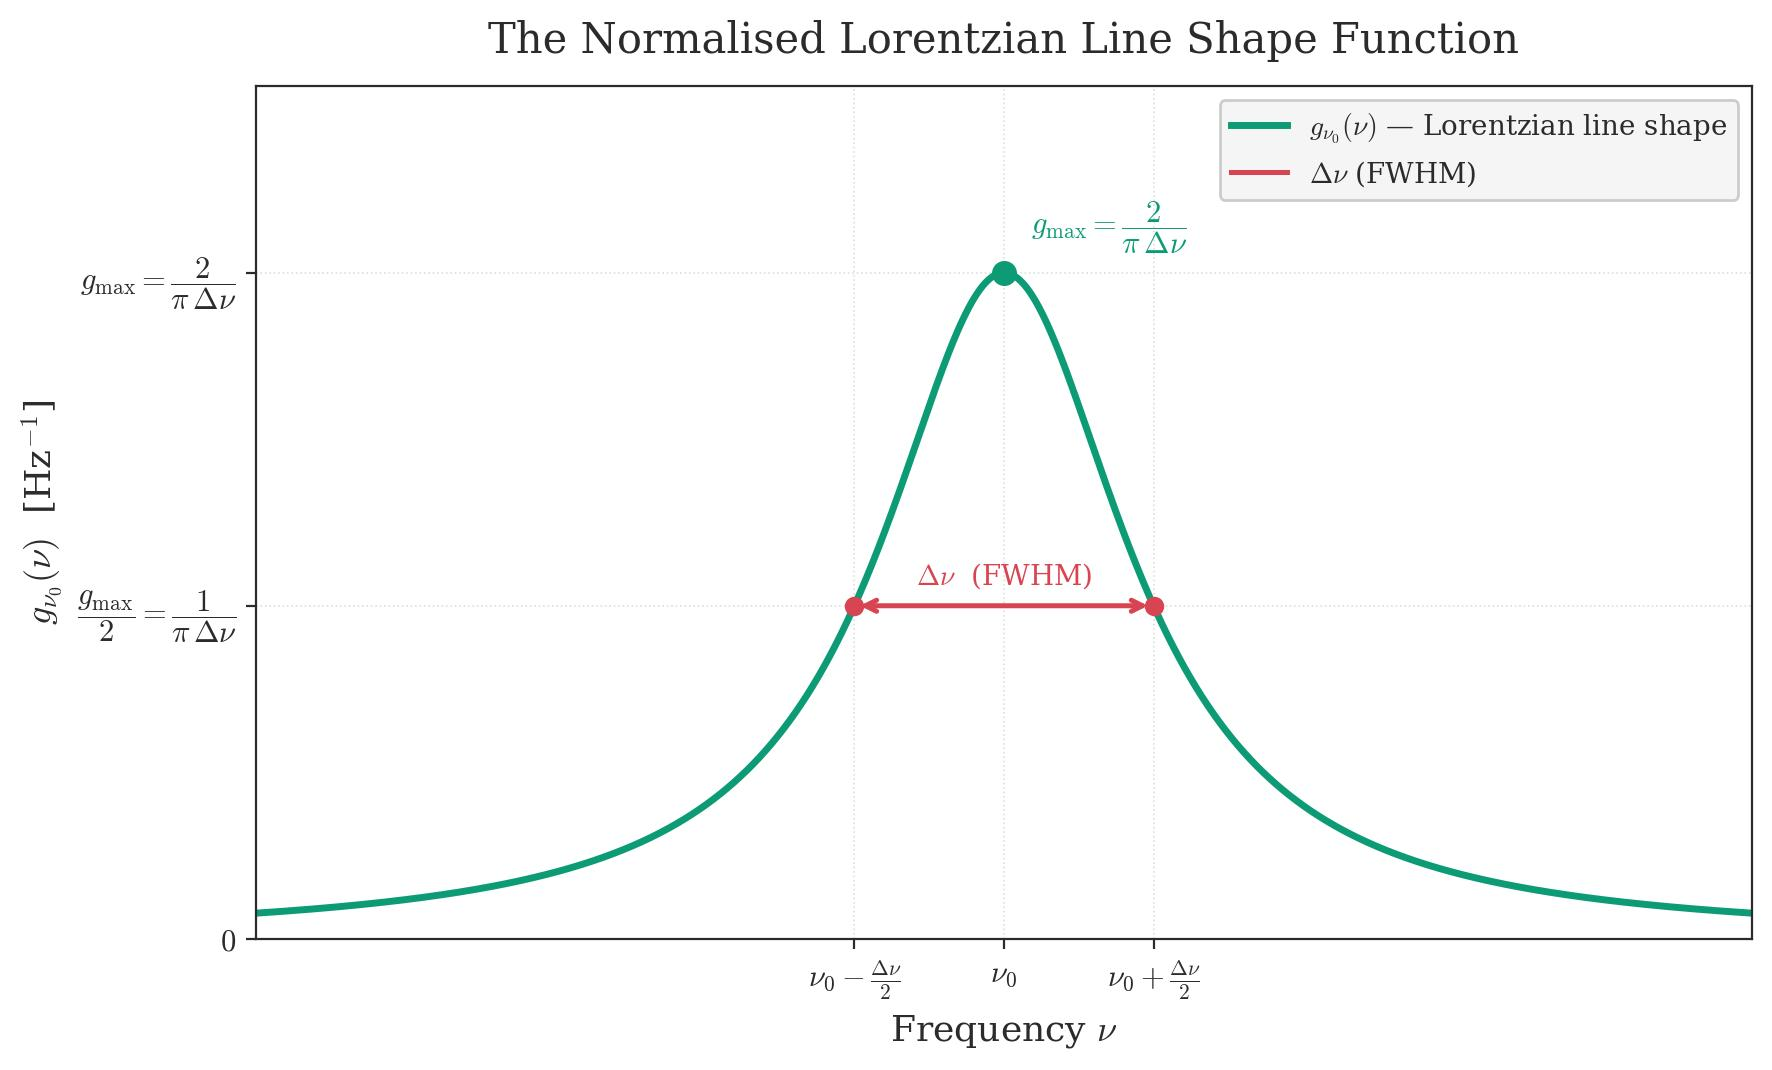
\includegraphics[width=0.65\textwidth]{Figures/Chapter 1/lineshape_function_lorentzian.jpg}
    \caption{The Line Shape Function: The Lorentzian distribution normalised to unity, explicitly marking the peak amplitude $g_{\max} = 2/\pi\Delta\nu$ and the Full Width at Half Maximum $\Delta\nu$.}
\end{figure}

Having proven what $\Delta\nu$ represents geometrically, we now ask what sets its actual size physically. The resonance bandwidth is fundamentally fixed by the total radiation lifetime of the excited state: $\Delta\nu = 1/(2\pi\tau_t)$.

This inverse relationship is not a coincidence; it is a direct consequence of the Heisenberg Uncertainty Principle in its energy-time form, which dictates that $\Delta E \Delta t \ge \hbar/2$. Because a photon's energy is irrevocably tied to its frequency by $E = h\nu$, an uncertainty in energy translates perfectly to an uncertainty in the emitted frequency spread ($\Delta E = h\Delta\nu$). If an atom's excited state decays rapidly (short $\tau_t$), the emission event is violently brief — the photon's energy is thus highly uncertain, forcing a massive frequency spread and a broad, flat Lorentzian. Conversely, a long-lived excited state — such as a metastable lasing level — gives the atom time to ring for millions of coherent cycles before decaying. The photon energy becomes highly well-defined, resulting in a tall, aggressively narrow spectral line.

The consequence of this fundamental quantum limit is captured neatly by the \textbf{lifetime-bandwidth product}, which sets a fixed universal constant for any homogeneously broadened transition: $\Delta\nu \cdot \tau_t = 1/(2\pi)$. Notice that multiplying this by $h$ yields $h\Delta\nu\,\tau_t = h/(2\pi) = \hbar$, which safely satisfies the $\ge \hbar/2$ Heisenberg bound. No matter how broad or narrow the line, two things always hold: as $\Delta\nu$ grows, the peak $g_{\max} = 2/(\pi\Delta\nu)$ drops proportionally, keeping the total area under $g_{\nu_0}(\nu)$ conserved at exactly one.

With the line shape fully characterised, we can now connect $g_{\nu_0}(\nu)$ to a physically intuitive per-atom quantity: the absorption cross section.

% ----------------------------------------------------------
%  Section 3: Absorption Cross Section
% ----------------------------------------------------------
\section{Absorption Cross Section}


\subsection{Definition and Physical Picture}

The \textbf{absorption cross section} $\sigma$ is a quantity that tells us how strongly a single molecule (or equivalently, for our purposes, a single atom in a gas) interacts with light at frequency $\nu$. In the geometric picture used here, it is represented as an \emph{effective interaction area}: if the path of the light intersects that area, the event is counted as absorption. It is therefore not the literal physical size of the atom, but a compact way to describe the absorption strength of one atom at a given frequency.

Think of it this way. We have a large material through which light is passing. Inside that material, each atom contributes its own effective area $\sigma$. The total absorption in the material is then the cumulative effect of all these microscopic interaction areas distributed throughout the medium. This allows us to represent a complicated distributed medium as a collection of discrete absorbers, each characterised by the same per-atom cross section at that frequency.

\begin{figure}[H]
    \centering
    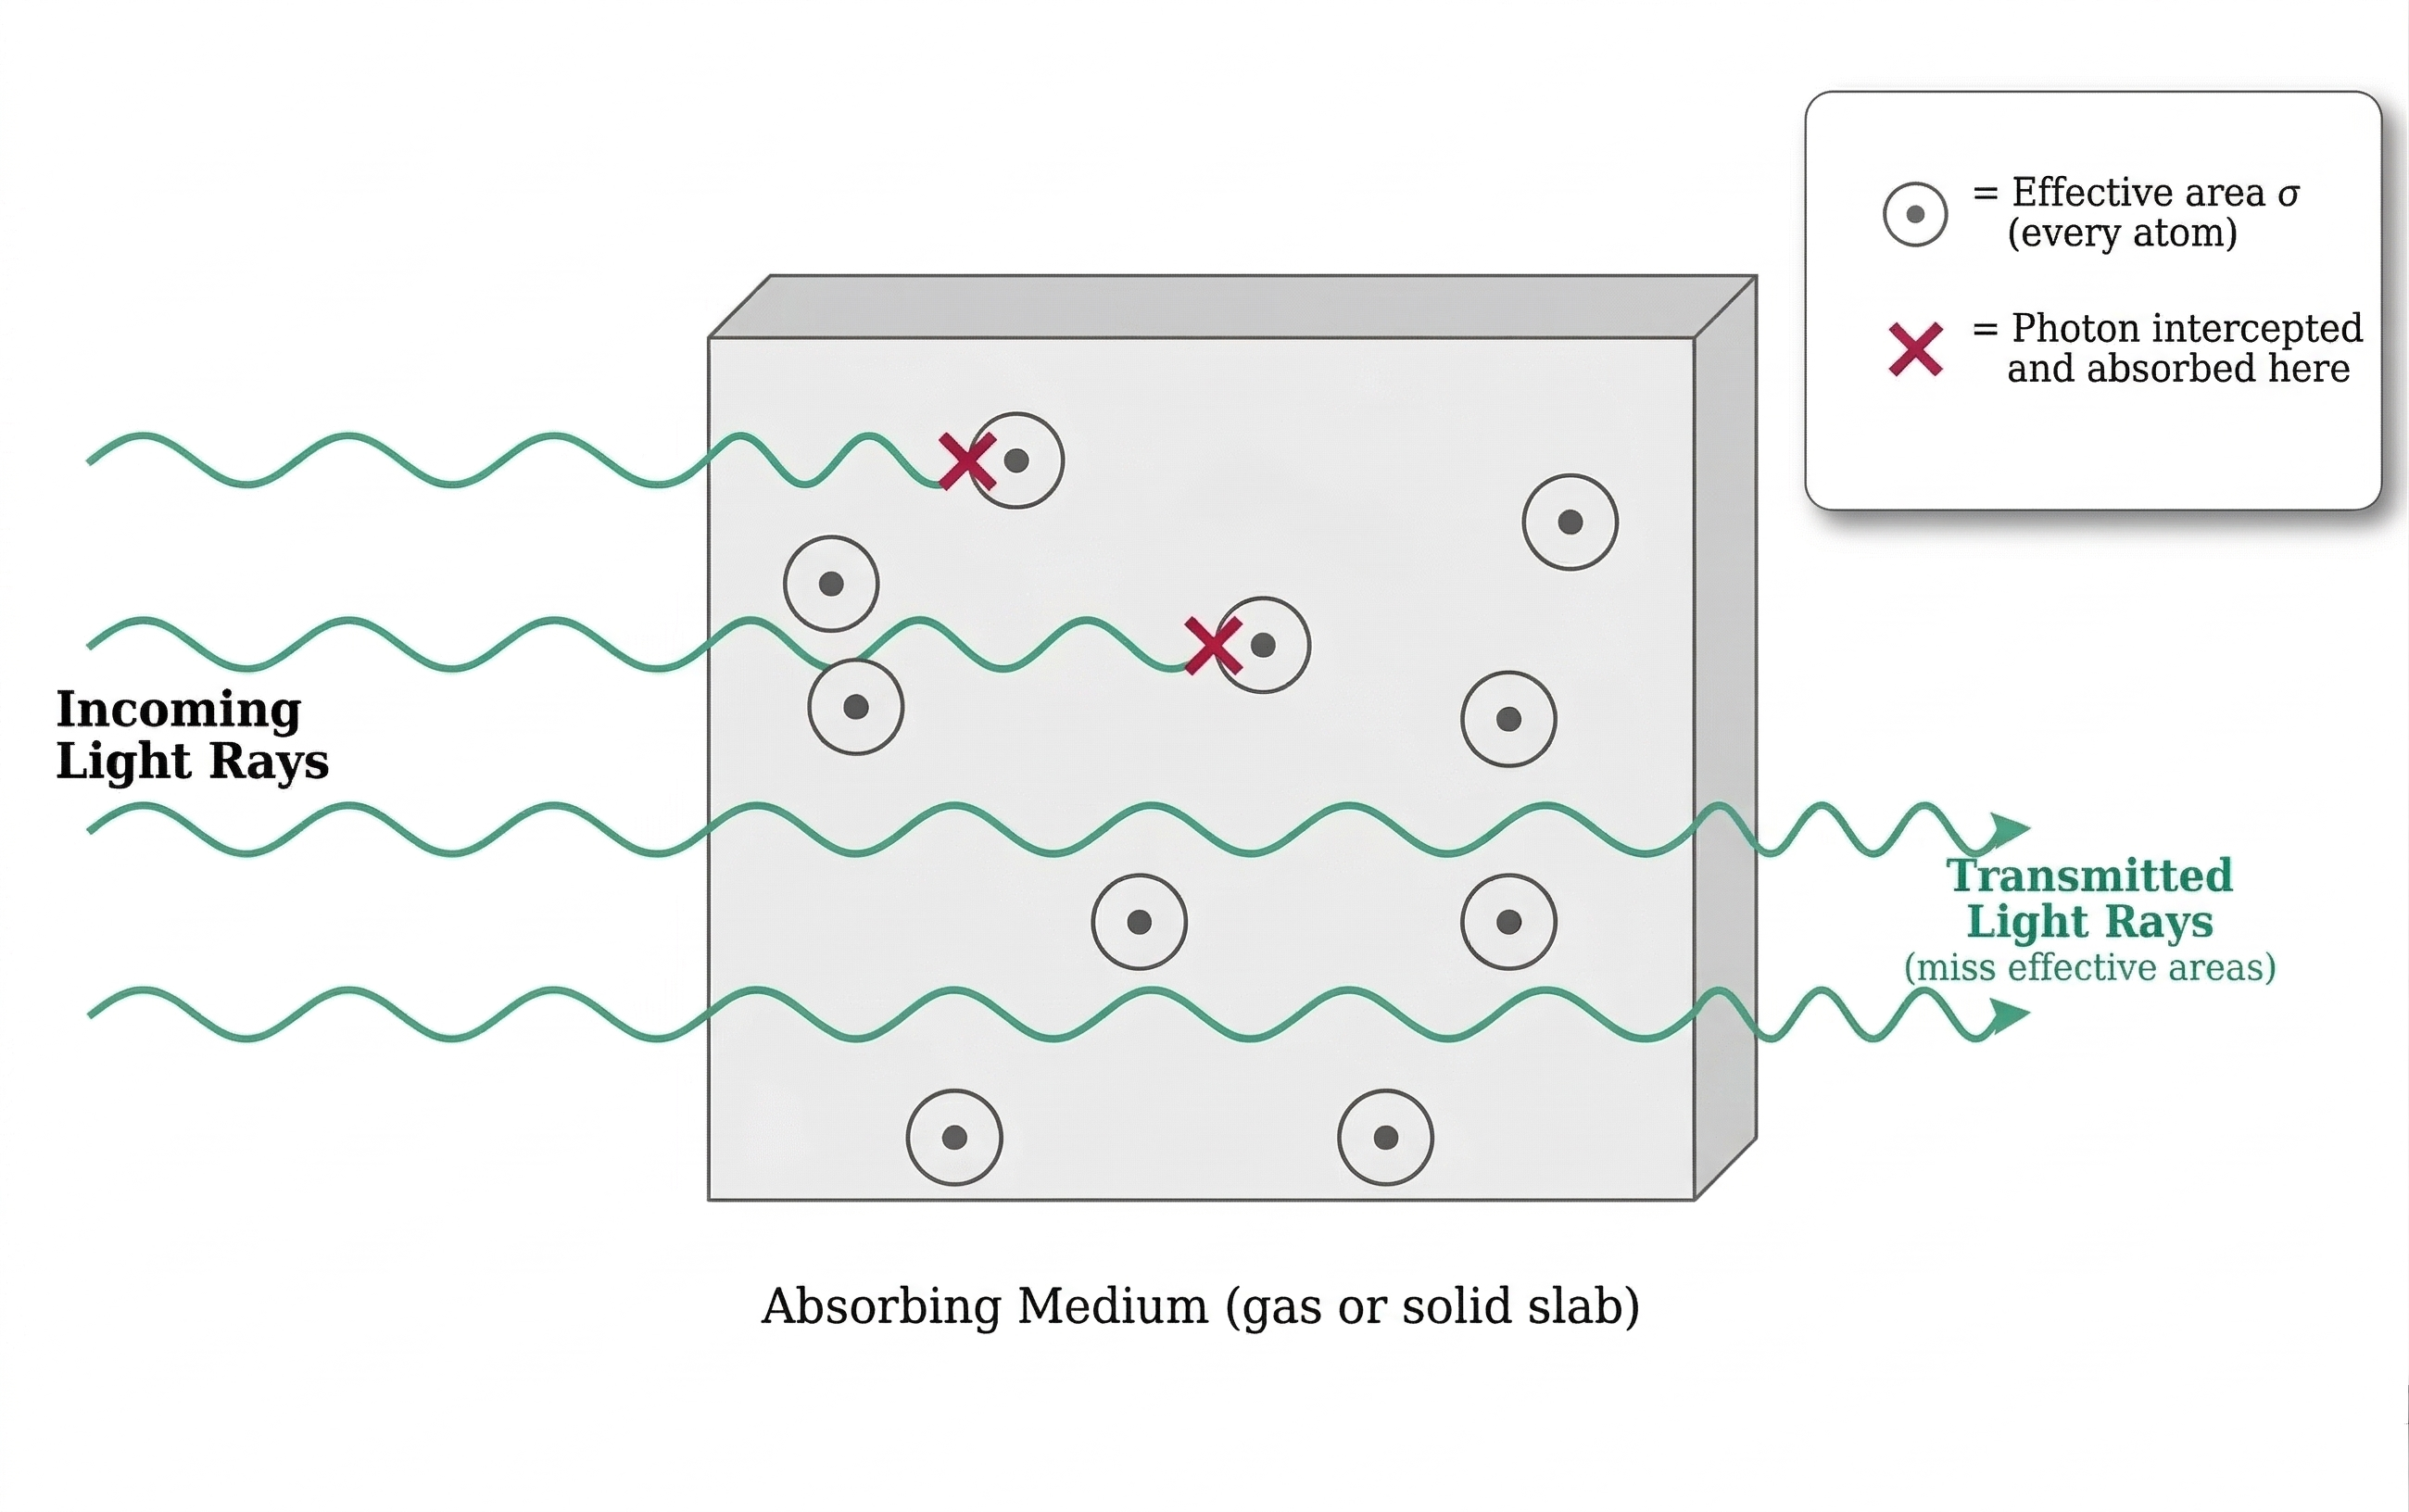
\includegraphics[width=0.65\textwidth]{Figures/Chapter 1/absorption_cross_section.jpg}
    \caption{The Absorption Cross Section: a conceptual picture in which each atom contributes the same effective interaction area $\sigma$; paths that intersect this area are absorbed, while paths that miss all such areas are transmitted.}
\end{figure}

The term we use is $\sigma$, and its unit is area (e.g., $\text{m}^2$ or $\text{cm}^2$). We can extract the exact mathematical formula for this cross section directly from the macroscopic absorption coefficient we derived earlier.

\subsection{Deriving the Explicit Formula for \texorpdfstring{$\sigma$}{sigma(nu)}}

The macroscopic absorption coefficient naturally takes the form:
\begin{equation*}
    \alpha = \frac{3N_A\,\lambda^2}{8\pi\,\tau_r}\,g_{\nu_0}(\nu)
\end{equation*}

This formula cleanly factors into the atomic number density $N_A$ explicitly scaled by a purely frequency-dependent per-atom term. We can physically group it as:
\begin{equation*}
    \alpha = N_A \cdot \left[ \frac{3\lambda^2}{8\pi\tau_r}\,g_{\nu_0}(\nu) \right]
\end{equation*}

We formally define this isolated per-atom factor as the \textbf{absorption cross section}:

\begin{keyresult}
    \begin{equation}
        \sigma = \frac{3\lambda^2}{8\pi\tau_r}\cdot g_{\nu_0}(\nu)
    \end{equation}
\end{keyresult}

And therefore, the macroscopic absorption coefficient directly relates to the microscopic cross section simply as:
\begin{keyresult}
    \begin{equation}
        \alpha = N_A\,\sigma
    \end{equation}
\end{keyresult}

The absorption cross section $\sigma$ is the per-atom absorption strength at frequency $\nu$. It carries two independent pieces of information encoded together: the \emph{spectral shape}, which comes entirely from $g_{\nu_0}(\nu)$ and tells us how the absorption is distributed across frequencies, and the \emph{overall magnitude}, which is fixed by $\lambda^2/\tau_r$ and tells us how strongly one atom interacts with the field in the first place.

The $\tau_r$ in the denominator reflects the core physical principle that emission and absorption are reciprocal processes. An atom with a short $\tau_r$ is strongly coupled to the field — it emits quickly, and equally, it absorbs efficiently — so its cross section is large. An atom with a long $\tau_r$ barely interacts with the field at all, so even though it is nominally resonant, it captures very little of the incoming light.

\begin{keyinsight}[Limiting Case: $\tau_r \to \infty$]
    If the radiative lifetime were infinite, the atom would have zero coupling to the electromagnetic field — it would never emit, and by the same token, never absorb. The formula correctly captures this: $\sigma \to 0$ as $\tau_r \to \infty$. This is not a breakdown of the physics; it is exactly what we expect from a perfectly stable state with no field interaction whatsoever.
\end{keyinsight}

Through $\alpha = N_A\,\sigma$, the per-atom cross section scales up to the macroscopic absorption coefficient. Let us now confirm physically why this product correctly maps to the fractional intensity decay we observe experimentally.

\subsection{Relating Intensity Change to the Cross Section}

Now that we have explicitly derived $\alpha = N_A\,\sigma$, let us verify that this mathematical separation makes physical sense by looking at how light intensity decays. Fundamentally, light intensity decays exponentially as it travels through a uniformly absorbing medium:
\begin{equation*}
    I(z) = I_0\, e^{-\alpha z} \qquad (\text{intensity at position } z)
\end{equation*}
The intensity at position $z + \Delta z$ is:
\begin{equation*}
    I(z + \Delta z) = I_0\, e^{-\alpha(z+\Delta z)} = I_0\, e^{-\alpha z}\, e^{-\alpha \Delta z}
\end{equation*}
This is the intensity that exits the material slab of thickness $\Delta z$.

\begin{figure}[H]
    \centering
    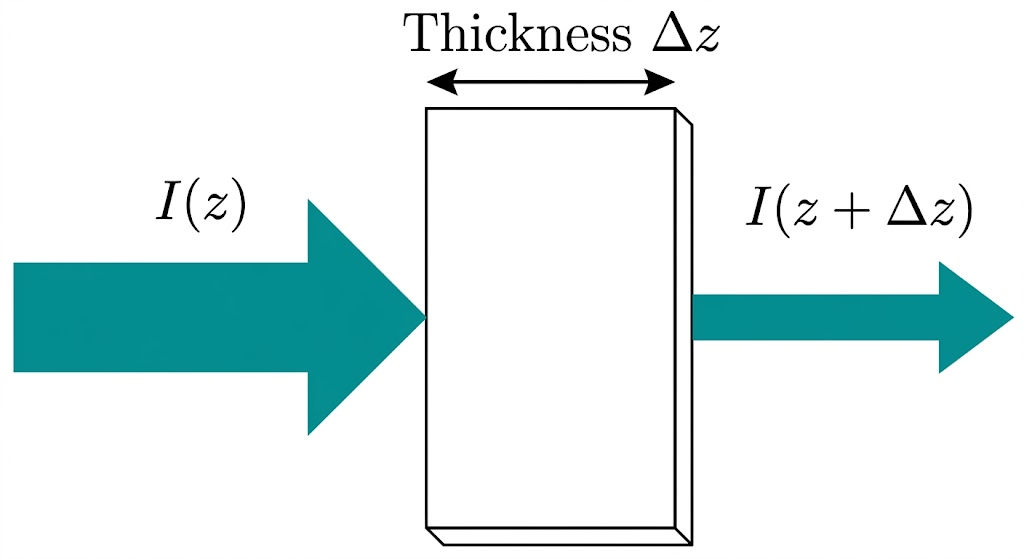
\includegraphics[width=0.5\textwidth]{Figures/Chapter 1/fractional_intensity_decay.jpg}
    \caption{Fractional Intensity Decay: Tracking the drop in wave intensity precisely across a differential material slice of thickness $\Delta z$.}
\end{figure}

The fractional change in intensity across this slab is:
\begin{gather*}
    \frac{\Delta I}{I} = \frac{I(z+\Delta z) - I(z)}{I(z)} = \frac{I_0 e^{-\alpha z} e^{-\alpha\Delta z} - I_0 e^{-\alpha z}}{I_0 e^{-\alpha z}} \notag \\
    = e^{-\alpha\Delta z} - 1
\end{gather*}

Now we apply the Taylor approximation $e^{-\alpha\Delta z} \approx 1 - \alpha\Delta z$, which is valid as long as $\alpha\Delta z \ll 1$:
\begin{equation*}
    \frac{\Delta I}{I} = (1 - \alpha\Delta z) - 1 = -\alpha\Delta z
\end{equation*}

Since we just firmly established that $\alpha = N_A\,\sigma$, we can seamlessly substitute this into the differential decay equation:
\begin{equation*}
    \frac{\Delta I}{I} = -N_A\,\sigma\,\Delta z
\end{equation*}

Now, $N_A$ is the number of atoms per unit volume (number density). We can write:
\begin{equation*}
    N_A = \frac{\text{number of atoms}}{\text{volume}} = \frac{\text{number of atoms}}{\text{area} \times \Delta z}
\end{equation*}
Substituting this expression:
\begin{gather*}
    \frac{\Delta I}{I} = -\frac{\text{number of atoms}}{\text{area} \times \Delta z} \cdot \sigma \cdot \Delta z \notag \\
    = -\frac{\text{number of atoms}}{\text{area}} \cdot \sigma
\end{gather*}

Therefore:
\begin{keyresult}
    \begin{equation}
        \frac{\Delta I}{I} = -\frac{\text{number of atoms}}{\text{area}} \cdot \sigma
    \end{equation}
\end{keyresult}

This result is dimensionless (as it must be, since $\Delta I/I$ is a ratio), which perfectly confirms that our mathematical formulation of $\sigma$ must indeed have units of area. This completes the physical picture: $\sigma$ represents a true macroscopic \emph{cross section}.

\textbf{Interpretation for a single atom:} If there is exactly one atom in the cross-sectional area, then:
\begin{equation*}
    \frac{\Delta I}{I} = -\frac{\sigma}{\text{area}}
\end{equation*}
This tells us that a single atom reduces the incident intensity by a fraction equal to its cross section divided by the total beam area.

\textbf{For more than one atom:} Each atom contributes independently, so:
\begin{equation*}
    \frac{\Delta I}{I} = -\frac{\sigma}{\text{area}} - \frac{\sigma}{\text{area}} - \cdots = -\frac{\text{number of atoms} \times \sigma}{\text{area}}
\end{equation*}
which is entirely consistent with what we derived above.

\begin{keyinsight}[Equivalence of Intensity and Power]
    Note that $\dfrac{\Delta I}{I} = \dfrac{\Delta P}{P}$, since $I = P/A$ and the area $A$ cancels. This means all the results we derived for fractional changes in intensity apply equally to fractional changes in optical power.
\end{keyinsight}

Now that we fully understand how a \emph{stationary} atom absorbs light and what the resulting line shape looks like, we must address a crucial physical reality: in gases, the atoms are \emph{not} stationary. They are moving. This changes the picture significantly.

% ----------------------------------------------------------
%  Section 4: Doppler Broadening
% ----------------------------------------------------------
\section{Doppler Broadening}

\subsection{Overview: Why Atom Motion Matters}

Everything derived so far implicitly assumed that the absorbing atoms are stationary. In that case, every atom sees the same incoming frequency, and the line shape function $g_{\nu_0}(\nu)$ is a complete and accurate spectral description of the medium.

In a \emph{gas}, however, this assumption breaks down. Gas atoms are in constant thermal motion — moving in random directions with a wide statistical distribution of speeds. Because of this relative motion between each atom and the incoming light wave, each atom perceives the wave at a slightly different frequency. This Doppler shift displaces every atom's absorption peak away from $\nu_0$ by an amount proportional to its velocity. Since an entire ensemble of atoms is present simultaneously, each moving at a different speed, their individual shifted peaks collectively smear the absorption profile across a band of frequencies. This is the phenomenon of \textbf{Doppler broadening}.

\subsection{The Doppler Frequency Shift}

Let us define the operational parameters:
\begin{itemize}
    \item $\nu_0$: the atom's true internal resonance. This is a fixed quantum property; the atom only absorbs light if the frequency \emph{it perceives in its own rest frame} is exactly $\nu_0$.
    \item $\nu_{\text{res}}$: the \textbf{source frequency} required to successfully excite this moving atom.
    \item $V$: the atom's velocity component along the axis of light propagation, with the sign convention $V > 0$ for motion away from the source (same direction as the light) and $V < 0$ for motion toward it.
\end{itemize}

Because the atom is moving relative to the incoming source wave, it perceives an inherent Doppler shift. The exact Doppler relation between the required source frequency ($\nu_{\text{res}}$) and the fixed atomic resonance ($\nu_0$) is:
\begin{equation*}
    \nu_{\text{res}} = \nu_0 \left(1 - \frac{V}{c}\right)^{-1}\!\left(1 - \frac{V^2}{c^2}\right)^{1/2}
\end{equation*}

Since thermal gas velocities are far below the speed of light ($V \ll c$), we simplify this exact formula using a first-order Taylor expansion in $x = V/c \ll 1$. We treat the two factors separately:
\begin{itemize}
    \item \textbf{The first factor:} $\left(1 - V/c\right)^{-1}$ — applying the standard approximation $(1-x)^{-1} \approx 1 + x$ yields $1 + V/c$.
    \item \textbf{The second factor:} $\left(1 - V^2/c^2\right)^{1/2}$ — the term $V^2/c^2$ is purely second-order. Therefore, to first order, this entire factor simply evaluates to $1$ and drops out.
\end{itemize}

Multiplying the two remaining factors back together:
\begin{equation*}
    \nu_{\text{res}} \approx \nu_0 \cdot \left[1 + \frac{V}{c}\right] \cdot [1]
\end{equation*}

This neatly isolates the final non-relativistic Doppler shift equation:

\begin{keyresult}
    \begin{equation}
        \nu_{\text{res}} = \nu_0\!\left(1 + \frac{V}{c}\right)
    \end{equation}
\end{keyresult}

The result $\nu_{\text{res}} = \nu_0(1 + V/c)$ has a direct physical reading. The correction factor $V/c$ specifies by exactly what fraction the source frequency must depart from $\nu_0$ to account for the atom's motion:
\begin{itemize}
    \item \textbf{$V > 0$ — atom moving away from the source:} The atom is fleeing the incoming wave, so the crests chase it and arrive at its location less frequently than they are emitted — the atom perceives a \textbf{red-shift}, a lower frequency than what the source emits. For the atom to still perceive exactly $\nu_0$ despite this downward distortion, the source must transmit at a frequency \emph{above} $\nu_0$. The formula confirms this: $\nu_{\text{res}} = \nu_0(1 + V/c) > \nu_0$.
    \item \textbf{$V < 0$ — atom moving toward the source:} The atom is running into the incoming wave, so the crests pile up and arrive more frequently — the atom perceives a \textbf{blue-shift}, a higher frequency than what the source emits. For the atom to perceive exactly $\nu_0$ despite this upward distortion, the source must transmit at a frequency \emph{below} $\nu_0$. The formula confirms this: $\nu_{\text{res}} = \nu_0(1 + V/c) < \nu_0$.
\end{itemize}
In both cases, the factor $(1 + V/c)$ in the formula automatically encodes the required adjustment — it shifts the firing frequency by precisely the amount needed so that the atom, despite its kinematic frequency distortion, perceives exactly its resonance $\nu_0$.

\begin{figure}[H]
    \centering
    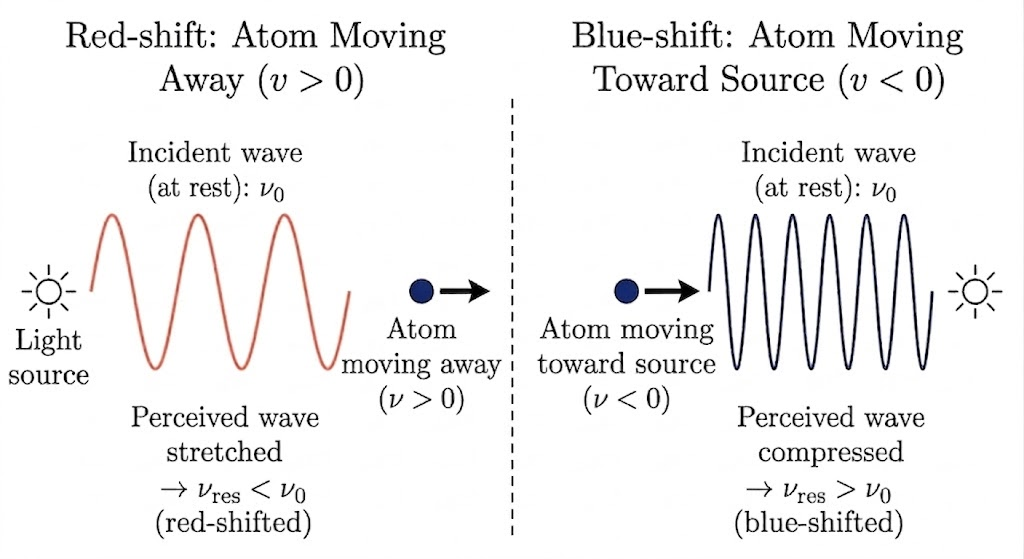
\includegraphics[width=0.6\textwidth]{Figures/Chapter 1/doppler_effect_gases.jpg}
    \caption{The Doppler Effect in Gases: Moving atoms perceive the incoming waves at shifted frequencies depending on whether they run away from (red-shift) or toward (blue-shift) the photon source.}
\end{figure}

In isolation, a single atom with velocity $V$ is completely characterised by this shift. The complication arises when every atom in the gas has a different $V$ drawn from a thermal distribution — and we must now build the collective picture.

\subsection{Building the Ensemble Line Shape}

A stationary, lifetime-limited atom exhibits a purely Lorentzian line shape centred at $\nu_0$:
\begin{equation*}
    g_{\nu_0}(\nu) = \frac{\Delta\nu/2\pi}{\left(\dfrac{\Delta\nu}{2}\right)^2 + \left(\nu - \nu_0\right)^2}
\end{equation*}

When the atom moves with velocity $V$, its perceived resonance centre shifts from $\nu_0$ to $\nu_{\text{res}} = \nu_0(1 + V/c)$, as we just derived. Crucially, the Lorentzian shape and its linewidth $\Delta\nu$ are completely unchanged by the motion — only the centre frequency relocates:
\begin{equation*}
    g_{\nu_{\text{res}}}(\nu) = \frac{\Delta\nu/2\pi}{\left(\dfrac{\Delta\nu}{2}\right)^2 + \left(\nu - \nu_0\!\left[1 + \dfrac{V}{c}\right]\right)^2}
\end{equation*}

This fully characterises the absorption profile of one atom moving at a fixed velocity $V$. In a real gas, however, no two atoms share the same velocity. Each atom has its own $V$, drawn from a thermal distribution, and therefore its own shifted Lorentzian centred at a slightly different frequency. The total absorption profile of the gas emerges from overlaying all of those shifted Lorentzians simultaneously — each one weighted by the probability that the gas actually hosts an atom moving at that particular velocity. Each atom's contribution to the total profile is therefore its shifted Lorentzian multiplied by the probability density of its velocity. The effective ensemble line shape $\bar{g}(\nu)$ is the continuous weighted average:
\begin{equation*}
    \bar{g}(\nu) = \int_{-\infty}^{\infty} g_{\nu_{\text{res}}}(\nu)\,f_V(V)\,dV
\end{equation*}
where $f_V(V)$ is the velocity probability density function. To evaluate this integral we need its explicit form, which we now derive.

\subsection{The Thermal Velocity Distribution}

From statistical mechanics, the velocity component of a gas atom along a single spatial axis obeys a Gaussian distribution at thermal equilibrium. This is a direct consequence of the \textbf{equipartition theorem}: each translational degree of freedom carries an average kinetic energy of $\frac{1}{2}k_BT$, and the unique normalised distribution satisfying this constraint is a Gaussian centred at zero velocity. The result, known as the \textbf{Maxwell-Boltzmann velocity distribution}, is:

\begin{keyresult}
    \begin{equation}
        f_V(V) = \frac{1}{\sqrt{2\pi}\,\sigma_V}\,\exp\!\left(-\frac{V^2}{2\sigma_V^2}\right)
    \end{equation}
\end{keyresult}

Where:
\begin{itemize}
    \item $V$: The velocity component of the gas atom along the axis of light propagation.
    \item $\sigma_V = \sqrt{k_BT/m}$: The standard deviation of the velocity distribution, where $T$ is the absolute gas temperature, $m$ is the mass of a single atom, and $k_B$ is Boltzmann's constant. It dictates the distribution's width, which broadens at higher temperatures and narrows for more massive atoms.
\end{itemize}

This distribution is perfectly normalised to unity ($\int_{-\infty}^{\infty} f_V(V)\,dV = 1$). As plotted in the distribution below, we can clearly see that its peak at $V = 0$ indicates that slowly-moving atoms are fundamentally the most abundant, with the population decaying exponentially as the absolute speed $|V|$ increases.

\begin{figure}[H]
    \centering
    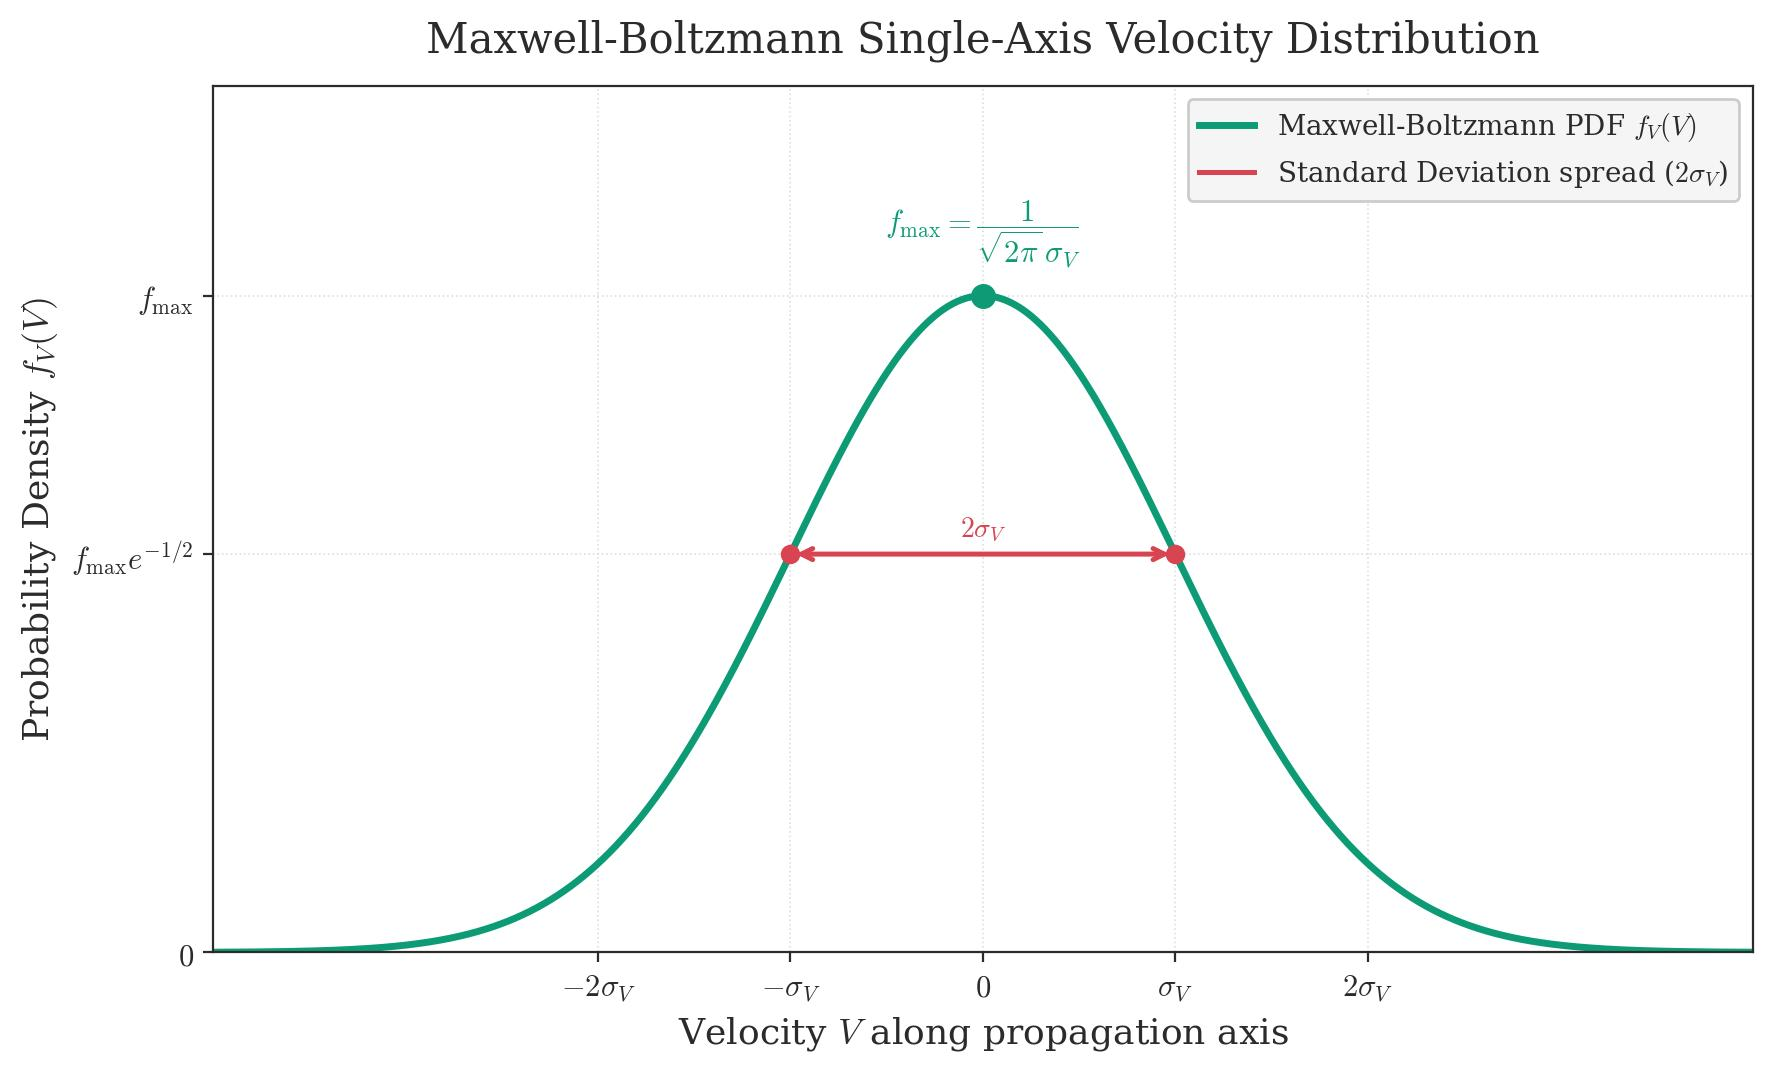
\includegraphics[width=0.65\textwidth]{Figures/Chapter 1/velocity_distribution.jpg}
    \caption{Velocity Distribution: The Maxwell-Boltzmann Gaussian PDF governing the thermal speeds of gas atoms along a single axis.}
\end{figure}

We now substitute the explicit forms of both the shifted Lorentzian $g_{\nu_{\text{res}}}(\nu)$ and the thermal Gaussian $f_V(V)$ directly into the weighted average integral:
\begin{equation}
    \bar{g}(\nu) = \int_{-\infty}^{\infty} \left[ \frac{\Delta\nu/2\pi}{\left(\dfrac{\Delta\nu}{2}\right)^2 + \left(\nu - \nu_0\!\left[1+\dfrac{V}{c}\right]\right)^2} \right] \cdot \left[ \frac{1}{\sqrt{2\pi}\,\sigma_V}\exp\!\left(-\frac{V^2}{2\sigma_V^2}\right) \right] dV \tag{I}
\end{equation}

This integral represents the mathematical \textbf{convolution of a Lorentzian and a Gaussian}. The resulting distribution is known as a \textbf{Voigt profile}.

Because the Lorentzian natural linewidth ($\Delta\nu$) and the Gaussian thermal spread ($\sigma_V$) cannot be separated inside the integral, the general case has no closed-form algebraic solution and must be evaluated numerically. However, we can still extract exact closed-form solutions by evaluating integral \textup{(I)} in its two extreme limits, which are dictated by the width $\sigma_V$. We will now analyze both of these distinct broadening regimes.

\subsubsection{Homogeneous Broadening — Negligible Doppler ($\sigma_V \to 0$)}

When temperature is low ($T \to 0$) and atomic velocities are negligible, essentially all atoms are stationary. All Doppler shifts vanish and their individual Lorentzians coalesce at exactly $\nu_0$, meaning the gas behaves as a spectrally uniform medium. Mathematically, this is captured by the velocity distribution collapsing to a single spike:
\begin{equation*}
    f_V(V) \to \delta(V)
\end{equation*}
Substituting into \textup{(I)} and applying the sifting property of the delta function:
\begin{equation*}
    \bar{g}(\nu) = \int_{-\infty}^{\infty} g_{\nu_{\text{res}}}(\nu)\,\delta(V)\,dV = g_{\nu_0}(\nu)
\end{equation*}
The delta function selects only the $V = 0$ term — the unshifted stationary-atom Lorentzian:
\begin{keyresult}
    \begin{equation}
        \bar{g}(\nu) = g_{\nu_0}(\nu) = \frac{\Delta\nu/2\pi}{\left(\dfrac{\Delta\nu}{2}\right)^2 + (\nu - \nu_0)^2} \qquad \text{(Lorentzian)}
    \end{equation}
\end{keyresult}

Under this \textbf{homogeneous broadening} limit, every single atom in the gas acts as a spectrally equivalent absorber — they all absorb at the same frequency and respond identically to any incoming light. The linewidth $\Delta\nu = 1/(2\pi\tau_t)$ is set entirely by the excited state's total lifetime $\tau_t$, with zero contribution from atomic motion.

\subsubsection{Inhomogeneous Broadening — Dominant Doppler ($\sigma_V \to \infty$)}
Now let's consider the opposite extreme. When the temperature of the gas is very high, the atoms fly around with an enormous spread of thermal velocities. This means each atom gets Doppler-shifted to a significantly different resonance frequency, so the gas as a whole absorbs over a very wide spectral window. Consequently, different velocity groups contribute to entirely different segments of the overall line shape.

The mathematical condition defining this extreme regime is:
\begin{equation*}
    \frac{\nu_0}{c}\sigma_V \gg \Delta\nu
\end{equation*}

It is crucial to explicitly unpack what this inequality represents:
\begin{itemize}
    \item \textbf{Where it came from:} We established that an atomic velocity $V$ induces a Doppler frequency shift of $\nu_0 \frac{V}{c}$. Because the thermal velocities within the gas are statistically distributed with a standard deviation $\sigma_V$, the resulting Doppler shifts intrinsically inherit a standard deviation of $\frac{\nu_0}{c}\sigma_V$. The left side therefore quantifies the macroscopic Doppler frequency spread across the entire gas ensemble.
    \item \textbf{The Physical Meaning:} This inequality formally compares two fundamentally distinct broadening mechanisms: the macroscopic Doppler spread of the gas ensemble (left) and the intrinsic natural linewidth of a single atom (right). Enforcing this condition defines a high-temperature regime where the thermal velocity distribution completely dominates the absorption profile. In this limit, the underlying Lorentzian width of any individual atom is rendered physically negligible.
    \item \textbf{The Mathematical Target:} The general line shape is a complex Voigt convolution lacking a closed-form solution. This extreme condition rigorously justifies taking the limit $\Delta\nu \to 0$. Collapsing the underlying Lorentzian into a Dirac delta function allows the intractable integral to instantly evaluate into a simple, closed-form Gaussian formula.
\end{itemize}

To execute this mathematical goal, we use a convenient tool called the Cauchy limit identity. It provides a formal way to write a Dirac delta function identically as the limit of a squeezed Lorentzian fraction:
\begin{equation*}
    \lim_{\epsilon \to 0} \frac{\epsilon}{\epsilon^2 + x^2} = \pi\,\delta(x)
\end{equation*}
This identity tells us that when the width $\epsilon$ of a Lorentzian goes to zero, the Lorentzian collapses into a delta function. This is exactly what is happening physically: as $\Delta\nu \to 0$, each atom's Lorentzian collapses into a spike.

To apply this, we first rewrite our single-atom Lorentzian $g_{\nu_\text{res}}(\nu)$ in a form that matches the left-hand side. We factor out $1/\pi$:
\begin{equation*}
    g_{\nu_\text{res}}(\nu)
    = \frac{\Delta\nu/2\pi}{\left(\dfrac{\Delta\nu}{2}\right)^2 + \left(\nu - \nu_0 - \nu_0\dfrac{V}{c}\right)^2}
    = \frac{1}{\pi}\cdot\frac{\Delta\nu/2}{\left(\dfrac{\Delta\nu}{2}\right)^2 + \left(\nu - \nu_0 - \nu_0\dfrac{V}{c}\right)^2}
\end{equation*}

We can now directly read off the correspondence with the Cauchy limit: set $\epsilon = \Delta\nu/2$ (the half-linewidth) and $x = \nu - \nu_0 - \nu_0 V/c$ (the frequency detuning from the atom's shifted resonance). Substituting these into the Cauchy limit as $\epsilon = \Delta\nu/2 \to 0$:
\begin{equation*}
    \lim_{\Delta\nu \to 0} g_{\nu_\text{res}}(\nu) = \frac{1}{\pi} \cdot \pi\,\delta(x) = \delta\!\left(\nu - \nu_0 - \nu_0\frac{V}{c}\right)
\end{equation*}

This mathematical result perfectly encodes our high-temperature physical simplification. By forcing the internal natural linewidth to zero, we are mathematically modelling each individual atom as an idealized, infinitely selective receiver. An atom travelling at velocity $V$ will now absorb incoming light exclusively at its precise Doppler-shifted resonance, $\nu_0(1 + V/c)$, and will remain completely transparent to all other frequencies. Its absorption profile has effectively collapsed from a continuous smeared curve into one perfectly sharp, singular frequency spike.

We now substitute this delta function approximation back into our general ensemble integral \textup{(I)}, replacing the full Lorentzian with the spike:
\begin{equation*}
    \bar{g}(\nu)
    = \int_{-\infty}^{\infty} \delta\!\left(\nu - \nu_0 - \nu_0\frac{V}{c}\right)
    \cdot \frac{1}{\sqrt{2\pi}\,\sigma_V}\exp\!\left(-\frac{V^2}{2\sigma_V^2}\right) dV
\end{equation*}

\begin{keyinsight}[The Sifting Property of the Dirac Delta]
    The sifting (or sampling) property is the defining characteristic of the Dirac delta function under integration. It dictates that integrating the product of any function $f(x)$ and a delta spike $\delta(x - x_0)$ simply evaluates the function at the spike's location:
    \begin{equation*}
        \int_{-\infty}^{\infty} f(x)\,\delta(x - x_0)\,dx = f(x_0)
    \end{equation*}
    Because the delta function is strictly zero everywhere except at exactly $x = x_0$, the integral destroys the entire continuum of $f(x)$ except for that one single point. It ``sifts'' through the function to pull out the exact target value $f(x_0)$, collapsing the integral into a simple algebraic substitution.
\end{keyinsight}

The delta function's argument in our integral currently contains the integration variable $V$ multiplied by a constant coefficient $\left(\frac{\nu_0}{c}\right)$. While the sifting property could technically be applied directly using the formal scaling identity $\delta(aV) = \frac{1}{|a|}\delta(V)$, it is mathematically cleaner to simply change variables to clear the coefficient. Let us define a new dummy integration variable $u$:
\begin{equation*}
    u \equiv \frac{\nu_0}{c}\,V \quad\Longrightarrow\quad V = \frac{c}{\nu_0}\,u \quad\text{and}\quad dV = \frac{c}{\nu_0}\,du
\end{equation*}

Since $\nu_0$ and $c$ are strictly positive constants, the limits of integration are unchanged ($V: -\infty \to \infty$ maps cleanly to $u: -\infty \to \infty$). Substituting both $V = \frac{c}{\nu_0}u$ and $dV = \frac{c}{\nu_0}du$ into the integral yields:
\begin{equation*}
    \bar{g}(\nu)
    = \int_{-\infty}^{\infty} \delta(\nu - \nu_0 - u)
    \cdot \frac{1}{\sqrt{2\pi}\,\sigma_V}\exp\!\left(-\frac{u^2 c^2}{2\sigma_V^2\nu_0^2}\right) \frac{c}{\nu_0}\,du
\end{equation*}

Because the delta function is perfectly symmetric ($\delta(-y) = \delta(y)$), our term $\delta(\nu - \nu_0 - u)$ is mathematically identical to $\delta(u - (\nu - \nu_0))$. It therefore acts as a pure sifting function triggering exactly at $u = \nu - \nu_0$. By applying the sifting property, we pick out precisely this corresponding value of $u$ from the remaining exponential integrand, causing the integral to structurally collapse:
\begin{equation*}
    \bar{g}(\nu) = \frac{c}{\nu_0} \cdot \frac{1}{\sqrt{2\pi}\,\sigma_V}\exp\!\left(-\frac{(\nu-\nu_0)^2 c^2}{2\sigma_V^2\nu_0^2}\right)
\end{equation*}

This expression already is a Gaussian, but it doesn't look like one yet because the constants are scattered. Let's group them. We pull the $c/\nu_0$ factor into the denominator under the square root:
\begin{equation*}
    \bar{g}(\nu)
    = \frac{1}{\sqrt{2\pi}\!\left(\dfrac{\nu_0}{c}\sigma_V\right)}
    \exp\!\left(-\frac{(\nu-\nu_0)^2}{2\!\left(\dfrac{\nu_0}{c}\sigma_V\right)^2}\right)
\end{equation*}

This equation is mathematically a perfect Gaussian, centered at $\nu_0$, whose standard deviation is exactly the grouped term $\frac{\nu_0}{c}\sigma_V$. We formally define this term as the \textbf{Doppler broadening parameter}, $\sigma_D$, allowing us to write the final ensemble line shape in its cleanest form:
\begin{keyresult}
    \begin{gather}
        \bar{g}(\nu) = \frac{1}{\sqrt{2\pi}\,\sigma_D}\exp\!\left(-\frac{(\nu-\nu_0)^2}{2\sigma_D^2}\right) \qquad \text{(Gaussian)} \\[1ex]
        \sigma_D = \frac{\nu_0}{c}\,\sigma_V \nonumber
    \end{gather}
\end{keyresult}
where $\sigma_D$ operates as the standard deviation of the macroscopic absorption profile in frequency units. It quantifies how significantly the Doppler shifts spread the gas's overall absorption spectrum by scaling the previously defined underlying thermal velocity spread, $\sigma_V = \sqrt{k_BT/m}$.

The most practically useful measure of a line's width is its Full Width at Half Maximum (FWHM), $\Delta\nu_D$, since this is what can be directly measured. We find it by asking: at what frequencies does the profile fall to half its peak value?

The peak of our Gaussian is at $\nu = \nu_0$ and has the value $1/(\sqrt{2\pi}\,\sigma_D)$. The half-maximum condition on the exponential factor is:
\begin{equation*}
    \exp\!\left(-\frac{(\nu-\nu_0)^2}{2\sigma_D^2}\right) = \frac{1}{2}
\end{equation*}

Taking the natural logarithm of both sides:
\begin{equation*}
    -\frac{(\nu-\nu_0)^2}{2\sigma_D^2} = -\ln 2
\end{equation*}

Solving for the detuning $(\nu - \nu_0)$:
\begin{equation*}
    (\nu-\nu_0)^2 = 2\sigma_D^2\ln 2 \quad\Longrightarrow\quad \nu = \nu_0 \pm \sqrt{2\ln 2}\cdot\sigma_D
\end{equation*}

The total width between the two half-maximum points is strictly twice this detuning:
\begin{equation*}
    \Delta\nu_D = 2 \cdot \sqrt{2\ln 2}\;\sigma_D
\end{equation*}

Which cleanly simplifies to:
\begin{keyresult}
    \begin{equation}
        \Delta\nu_D = \sqrt{8\ln 2}\;\sigma_D
    \end{equation}
\end{keyresult}

Physically, this mathematically confirms the core mechanism of \textbf{inhomogeneous broadening}: \emph{the gas is spectrally not a single entity, but a continuum of isolated velocity groups}. Because thermal motion scatters their individual resonance spikes across a vast spectral band, the tiny natural linewidth ($\Delta\nu$) of any single atom is completely washed out. The observed profile and its measurable linewidth $\Delta\nu_D$ are purely macroscopic statistical phenomena — they emerge entirely from the thermal velocity distribution and carry no information whatsoever about the internal quantum mechanics of the individual atoms.

\begin{figure}[H]
    \centering
    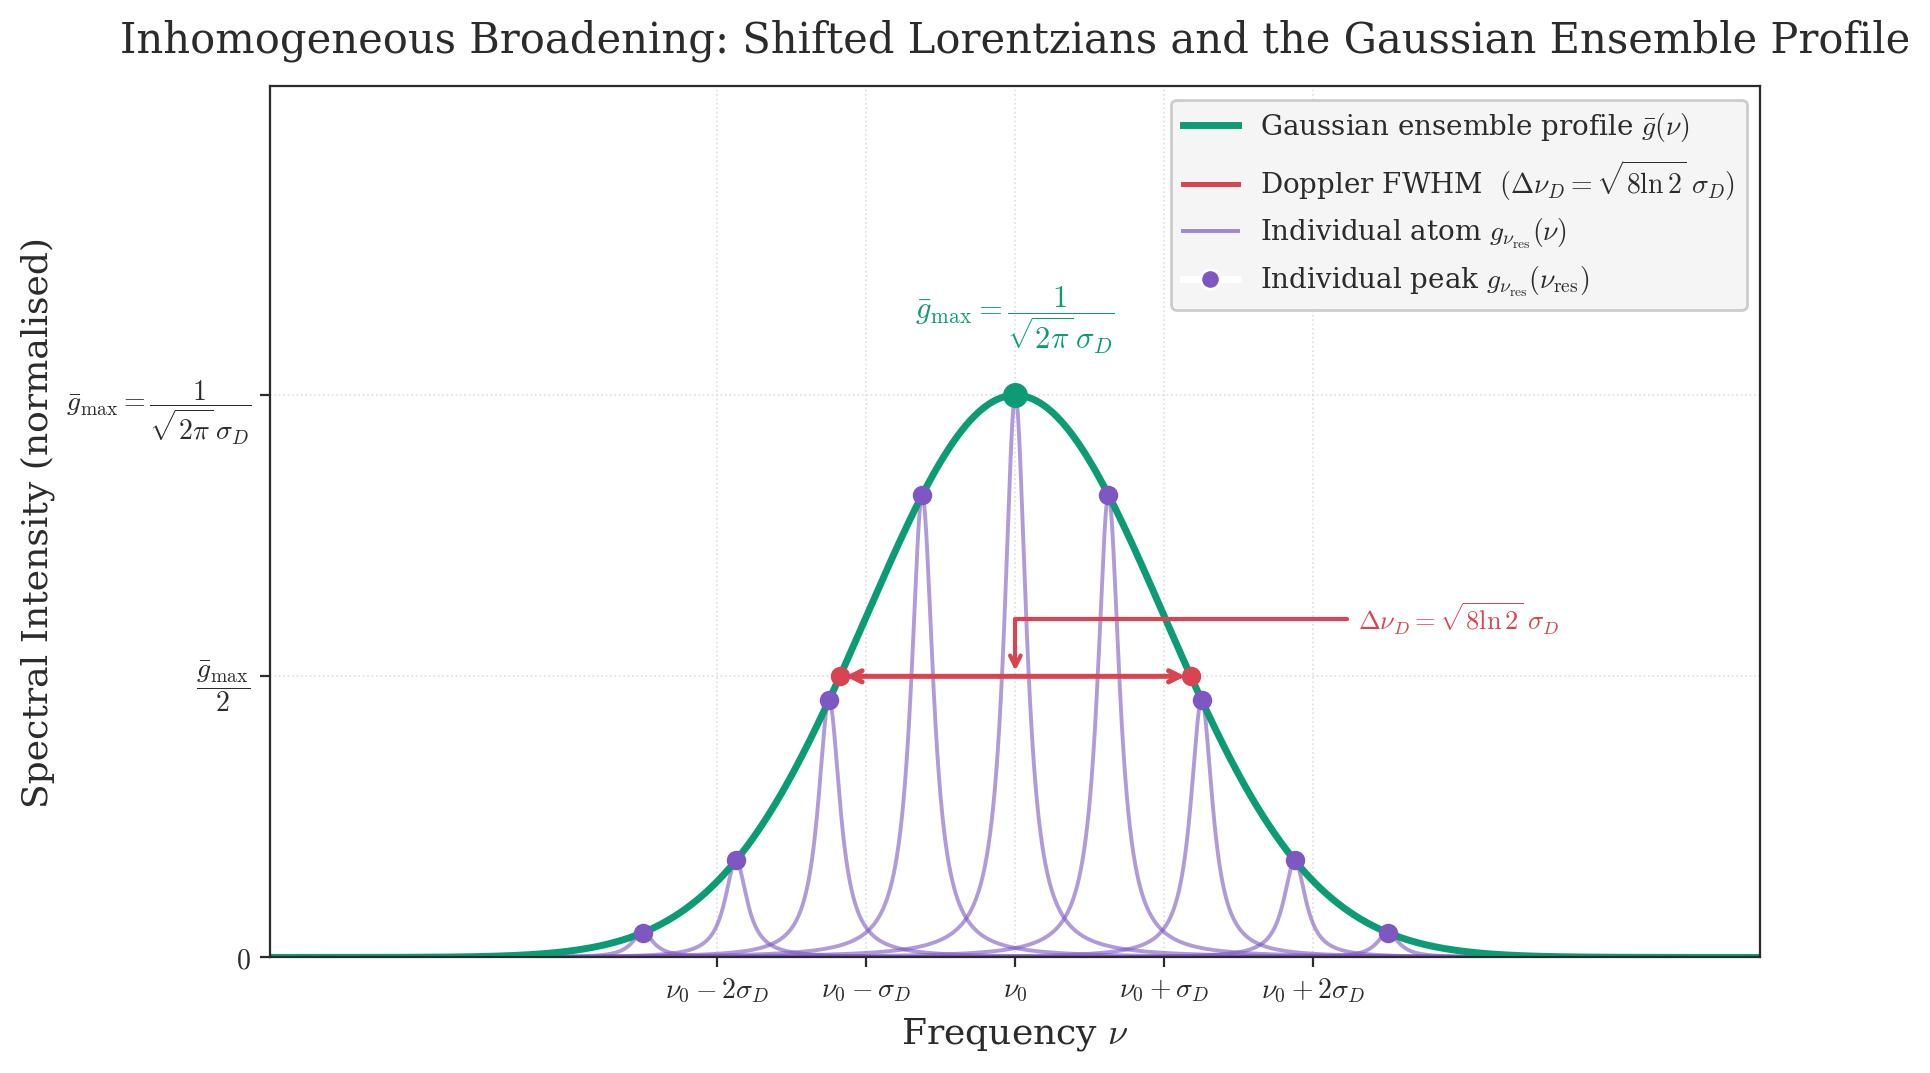
\includegraphics[width=0.65\textwidth]{Figures/Chapter 1/inhomogeneous_broadening.jpg}
    \caption{Inhomogeneous Broadening: Each individual atom contributes a narrow Doppler-shifted Lorentzian at its own resonance frequency. Their collective superposition constructs a broad Gaussian ensemble profile.}
\end{figure}

\newpage

\begin{keyinsight}[Homogeneous vs.\ Inhomogeneous Broadening]
    The distinction is not merely a matter of line shape — it reflects whether or not all atoms in the gas participate identically.
    \begin{itemize}
        \item In \textbf{homogeneous broadening}, all atoms are spectrally identical. Any incoming light frequency interacts with every atom equally. The medium is spectrally uniform.
        \item In \textbf{inhomogeneous broadening}, the ensemble is spectrally partitioned by velocity. A laser at a specific frequency only interacts with the narrow velocity subgroup that is Doppler-shifted into resonance with it — the remaining atoms are completely transparent to that frequency.
    \end{itemize}
    This distinction becomes critical when we study laser gain: an inhomogeneously broadened gain medium can support simultaneous oscillation at multiple laser frequencies, each burning its own spectral hole into a distinct velocity class.
\end{keyinsight}

In most practical gas systems at room temperature, the Doppler contribution dominates and the Gaussian approximation is entirely valid. As a concrete example, in a He-Ne gas discharge at 300\,K, the thermal velocity spread gives $\sigma_D \approx 750$\,MHz at the 633\,nm line — compared to the natural linewidth of only $\sim$10\,MHz. The Gaussian profile completely swamps the Lorentzian; a full Voigt treatment is only necessary when both contributions are comparable.

With $\bar{g}(\nu)$ now fully derived, the entire spectral framework developed earlier requires no structural modification. Every formula — from the absorption cross section $\bar{\sigma}(\nu) = \frac{3\lambda^2}{8\pi\tau_r}\bar{g}(\nu)$ to the macroscopic absorption coefficient $\alpha = N_A\bar{\sigma}(\nu)$ — carries over identically. The only change is which line shape $\bar{g}(\nu)$ is substituted: a Lorentzian in the homogeneous lifetime-limited regime, a Gaussian in the inhomogeneous Doppler-dominated regime, or the full Voigt integral \textup{(I)} in the general intermediate case. With the spectral framework now complete for both broadening regimes, we are ready to address one final, fundamental question: can $\alpha$ ever become negative?

% ----------------------------------------------------------
%  Section: Why the Classical Model Cannot Produce Gain
% ----------------------------------------------------------
\section{Why the Classical Model Cannot Produce Gain}

Before closing the classical treatment, let us make one final, crucial observation regarding our fundamental macroscopic absorption coefficient:
\begin{equation*}
    \alpha = \frac{N_A\,e^2}{4\varepsilon_0\,m\,n_b\,c_0}\cdot g_{\nu_0}(\nu)
\end{equation*}
Every single factor here is strictly positive: $N_A$, $e^2$, $\varepsilon_0$, $m$, $n_b$, $c_0$ are all fundamental constants or densities, and $g_{\nu_0}(\nu)$ is a Lorentzian probability density that is positive everywhere. There is therefore absolutely no way for $\alpha$ to ever become negative. A strictly positive $\alpha$ dictates exponential power decay via $P(z) = P(0)e^{-\alpha z}$, meaning the classical electron oscillator is fundamentally incapable of producing optical amplification — no matter what frequency, material, or density we choose.

\begin{figure}[H]
    \centering
    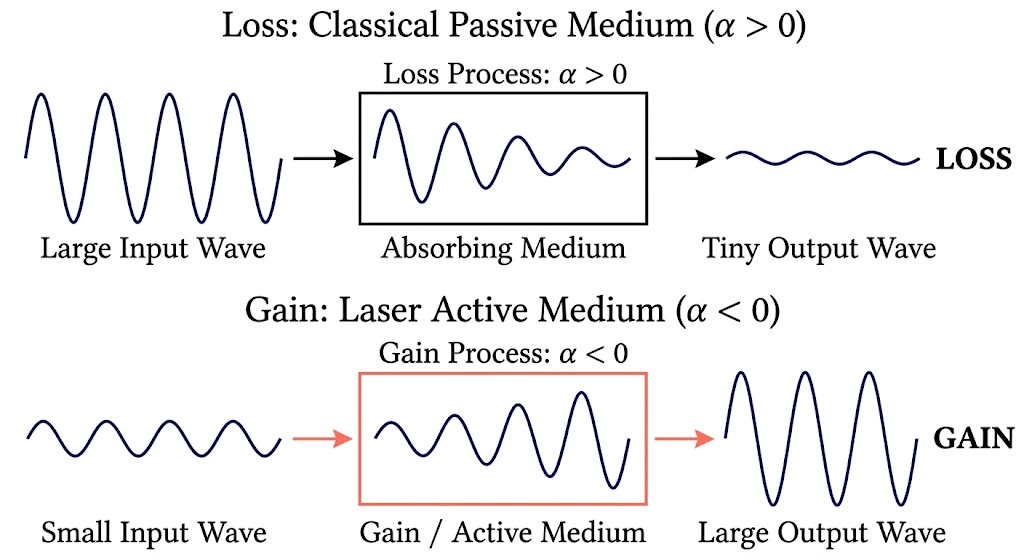
\includegraphics[width=0.6\textwidth]{Figures/Chapter 1/loss_vs_gain.jpg}
    \caption{Loss vs. Gain: The classical electron oscillator inherently enforces energy decay ($\alpha > 0$), mathematically forbidding the exponential amplification ($\alpha < 0$) required for lasers.}
\end{figure}

This is precisely why we must now move to the next level of description. The models ahead — starting with Einstein's rate equation model — will show us how to flip $\alpha$ to a negative value (gain instead of loss), leading ultimately to a complete understanding of how a laser works. All the phenomena we studied classically — the line shape, the cross section, the broadening — will reappear in those models, but now enriched with the mechanisms that allow both absorption \emph{and} amplification.
